\RCS$Revision: $
\RCS$HeadURL: $
\RCS$Id: $

%_______________________________________________________________________________
%_______________________________________________________________________________
%_______________________________________________________________________________

% Typesetting
\newcommand\T{\rule{0pt}{2.6ex}}
\newcommand\B{\rule[-1.2ex]{0pt}{0pt}}
\newcommand{\ph}[1]{\phantom{#1}}

% Symbols
\newcommand{\tf}{\ensuremath{\mathcal{R}}\xspace}
\newcommand{\cls}{\ensuremath{\text{CL}_\text{s}}\xspace}
\newcommand{\dm}{\ensuremath{{\Delta}m}\xspace}
\newcommand{\higgsmass}{\ensuremath{m_{\textrm{H}}}\xspace}
\newcommand{\jet}[1]{\ensuremath{\text{j}_\text{#1}}\xspace}
\newcommand{\PASQ}{\ensuremath{\overline{\widetilde{\cmsSymbolFace{q}}}}\xspace} 

% Variables
\newcommand{\Et}{\ensuremath{{E_{\text T}}}\xspace}
\newcommand{\njet}{\ensuremath{n_{\text{jet}}}\xspace}
\newcommand{\nb}{\ensuremath{n_{\text{b}}}\xspace}
\newcommand{\scalht}{\ensuremath{H_{\text{T}}}\xspace}
\newcommand{\scalst}{\ensuremath{\mathcal{E}_\text{T}}\xspace}
\newcommand{\mht}{\ensuremath{H_{\text{T}}^{\text{miss}}}\xspace}
\newcommand{\ptmiss}{\ensuremath{p_{\text{T}}^{\kern1pt\text{miss}}}\xspace}
\newcommand{\dst}{\ensuremath{\Delta\scalst}\xspace}
\newcommand{\alphat}{\ensuremath{\alpha_{\text{T}}}\xspace}
\newcommand{\bdphi}{\ensuremath{\Delta\phi^{*}_\text{min}}\xspace}
\newcommand{\bdphimod}{\ensuremath{\Delta\phi^{*_{\, 25}}_\text{min}}\xspace}
\newcommand{\minchi}{\ensuremath{\chi_\text{min}}\xspace}
\newcommand{\mhtmet}{\ensuremath{\mht / \ptmiss}\xspace}

% Selections
\newcommand{\jets}{\ensuremath{\text{jets}}}
\newcommand{\mj}{\ensuremath{\mu + \jets}\xspace}
\newcommand{\mmj}{\ensuremath{\mu\mu + \jets}\xspace}
\newcommand{\mmjpm}{\ensuremath{\mu^\pm\mu^\mp + \jets}\xspace}
\newcommand{\gj}{\ensuremath{\gamma + \jets}\xspace}

% Processes
\providecommand{\PSl}{\ensuremath{\widetilde{\ell}}\xspace}
\newcommand{\zmumu}{\ensuremath{\cPZ \to \mu\mu}\xspace}
\newcommand{\znunu}{\ensuremath{\cPZ \to \cPgn\cPagn}\xspace}
\newcommand{\zj}{\ensuremath{\cPZ + \jets}\xspace}
\newcommand{\zmumuj}{\ensuremath{\cPZ (\to \mu\mu) + \jets}\xspace}
\newcommand{\znunuj}{\ensuremath{\cPZ (\to \cPgn\cPagn) + \jets}\xspace}
\newcommand{\wj}{\ensuremath{\PW + \jets}\xspace}
\newcommand{\wmj}{\ensuremath{\PW (\to \mu\nu) + \text{jets}}\xspace}
\newcommand{\wlj}{\ensuremath{\PW (\to \ell\nu) + \text{jets}}\xspace}
\newcommand{\ttw}{\ensuremath{\ttbar\PW}\xspace}
\newcommand{\ttz}{\ensuremath{\ttbar\cPZ}\xspace}
\newcommand{\lost}{\ensuremath{\ell_\textrm{lost}}\xspace}
\newcommand{\ra}{\ensuremath{\rightarrow}}

\newlength\cmsFigWidth
\newlength\cmsFigWidthTwo
\ifthenelse{\boolean{cms@external}}{\setlength\cmsFigWidth{0.49\textwidth}}{\setlength\cmsFigWidth{0.7\textwidth}}
\ifthenelse{\boolean{cms@external}}{\setlength\cmsFigWidthTwo{0.95\textwidth}}{\setlength\cmsFigWidthTwo{0.95\textwidth}}
\ifthenelse{\boolean{cms@external}}{\providecommand{\cmsLeft}{top\xspace}}{\providecommand{\cmsLeft}{left\xspace}}
\ifthenelse{\boolean{cms@external}}{\providecommand{\cmsRight}{bottom\xspace}}{\providecommand{\cmsRight}{right\xspace}}
\ifthenelse{\boolean{cms@external}}{\providecommand{\cmsTable}[1]{#1}}{\providecommand{\cmsTable}[1]{\resizebox{\textwidth}{!}{#1}}}

\newlength\cmsTableLabelSkip
\setlength\cmsTableLabelSkip{-1.2ex}

%_______________________________________________________________________________
%_______________________________________________________________________________
%_______________________________________________________________________________

\cmsNoteHeader{SUS-16-038}

\title{Search for natural and split supersymmetric scenarios in pp
  collisions at $\sqrt{s} = 13~\text{TeV}$ in all-jet final states}
%  using the $\alpha_\text{T}$ variable}

\address[cern]{CERN} 
\author[cern]{The CMS Collaboration}

\date{\today}

\abstract{A search for supersymmetry is performed in final states
  comprising one or more jets and missing transverse momentum from pp
  collisions at a centre-of-mass energy of $13~\text{TeV}$. The event
  data were recorded with the CMS detector at the CERN LHC in 2016 and
  correspond to an integrated luminosity of $35.9~\text{fb}^{-1}$.
  %
  %Several kinematic variables are used to suppress the multijet
  %background to a subdominant level with respect to all other standard
  %model backgrounds. Further Several kinematic variables are used to
  %provide signal-to-background discrimination. 
  A maximum-likelihood description of the data reveals that the number
  of candidate events is found to agree with the expected event counts
  from standard model processes.
  %
  The result is interpreted with simplified models of supersymmetry
  that assume the production of gluino or squark pairs and their
  prompt decay to SM particles and the neutralino.
  % 
  Gluinos and their daughter neutralinos are probed up to masses of X
  and Y\TeV, respectively. In the case of direct production of
  light-flavour-, bottom-, or top-squark pairs, masses up to X, Y, and
  Z\GeV are probed. 
  %
  The search employs standard techniques of event reconstruction, yet
  also provides sensitivity to simplified models of split
  supersymmetry that involve the production and decay of meta-stable
  composite states containing gluinos, known as R-hadrons. A lower
  mass bound of X\TeV is established for gluinos with lifetimes in the
  range from ${\approx}10^{-6}$ to ${\approx}10^{2}\unit{ns}$ for
  gluino-neutralino mass differences larger than 25\GeV. Gluino masses
  up to Y\TeV are probed for lifetimes of
  ${\approx}10^{-3}\unit{ns}$. The search provides coverage that is
  complementary to existing dedicated techniques at the LHC.  }

\hypersetup{ 
  pdfauthor={Robert Bainbridge, Eshwen Bhal, Shane Breeze, Oliver
    Buchmueller, Stefano Casasso, Matthew Citron, Adam Elwood, Henning
    Flaecher, Aran Garcia-Bellido, Christian Laner, Kin Ho Lo, Sarah
    Alam Malik, Bjoern Penning, Tai Sakuma, Dominic Smith, Alex
    Tapper}, 
  pdftitle={Search for natural and split supersymmetric scenarios in pp
  collisions at 13 TeV in all-jet final states},
  pdfsubject={CMS, supersymmetry, AlphaT},
  pdfkeywords={Supersymmetry, split, natural, long-lived gluinos, dark matter}
}

\maketitle

%_______________________________________________________________________________
%_______________________________________________________________________________
%_______________________________________________________________________________

\section{Introduction}
\label{sec:introduction}

Supersymmetry (SUSY)~\cite{ref:SUSY-1, ref:SUSY0, ref:SUSY3,
  ref:SUSY1} is an extension of the standard model (SM) of particle
physics that introduces at least one bosonic (fermionic) superpartner
for each fermionic (bosonic) SM particle that differ in spin by
one-half unit. SUSY potentially offers solutions for the unification
of the gauge coupling constants at a high
energy~\cite{Dimopoulos:1981yj, Ibanez:1981yh, Marciano:1981un}, a
dark matter (DM) candidate, and the gauge hierarchy
problem~\cite{ref:hierarchy1, ref:hierarchy2}. SUSY particles are
expected to be produced in pairs at the LHC, with heavy states
decaying to the lightest stable SUSY particle (LSP), under the
assumption of $R$-parity conservation~\cite{Farrar:1978xj}. The LSP is
assumed to be the neutralino $\PSGczDo$, a weakly interacting massive
particle and a viable DM candidate~\cite{Jungman:1995df,
  1674-1137-38-9-090001}.  So-called ``natural'' models that invoke
only a minimal fine-tuning of the bare Higgs boson mass parameter
require only the gluino $\PSg$, third-generation squarks, and a
higgsino-like $\PSGczDo$ at or near the electroweak
scale~\cite{ref:barbierinsusy}. The interest in natural models is
motivated by the discovery of a low-mass Higgs
boson~\cite{Aad:2012tfa, Chatrchyan:2012ufa, Chatrchyan:2013lba,
  Khachatryan:2014jba, Aad:2014aba, Aad:2015zhl}. The characteristic
signature of natural SUSY production at the LHC is a final state
containing an abundance of jets originating from the hadronization of
light- or heavy-flavour quarks, accompanied by significant missing
transverse momentum \ptvecmiss.

%%%%%%%%%%

An alternative class of models known as ``split''
SUSY~\cite{ArkaniHamed:2004fb, Giudice:2004tc} remove the requirement
of minimal fine tuning of model parameters related to the Higgs boson
mass -- in constrast to natural models -- yet preserve the appealling
aspects of gauge coupling unification and a DM candidate. In such a
model, only the fermionic superpartners, and a finely-tuned scalar
Higgs boson, may be realised at a mass scale that is kinematically
accessible at the LHC, while all other SUSY particles are
ultraheavy. Hence, within split SUSY models, the $\PSg$ decay is
suppressed due to highly virtual squark states. For $\PSg$ lifetimes
beyond $\mathcal{O}(1\unit{ps})$, the $\PSg$ hadronizes and forms a
bound state with SM particles known as an
R-hadron~\cite{Fairbairn:2006gg}, before eventually decaying to SM
particles and the \chiz. The lifetime of the $\PSg$ determines the
position of the decay of the R-hadron within the CMS detector, which
can lead to a striking experimental signature of displaced particle
vertices located at a significant distance from the primary
interaction point of the incoming proton beams, accompanied by
significant \ptvecmiss from the undetected \chiz particles.

%%%%%%%%%%%%%%

This paper presents a search for new physics processes in final states
with one or more energetic jets and significant \ptvecmiss. The search
is performed with a sample of proton-proton (pp) collision data at a
centre-of-mass energy of 13\TeV. The analysed data sample recorded by
the CMS experiment corresponds to an integrated luminosity of $35.9
\pm 0.9 \fbinv$. Earlier searches using the same technique have been
performed in pp collisions at $\sqrt{s} = 7$, 8, and
13\TeV~\cite{RA1Paper, RA1Paper2011, RA1Paper2011FULL, RA1Paper2012,
  RA1Parked, Khachatryan:2016dvc} by the CMS Collaboration. The data
analysed in this analysis is a factor ${\approx}16$ larger than that
presented in Ref.~\cite{Khachatryan:2016dvc}. The ATLAS and CMS
Collaborations have performed similar searches in all-jet final states
at $\sqrt{s} = 13\TeV$, of which the most constraining are described
in Refs.~\cite{Aaboud:2016zdn, Sirunyan:2017cwe, Sirunyan:2017kqq}.

The search strategy aims to provide sensitivity to a broad range of
SUSY-inspired and non-SUSY models that predict the existence of a DM
candidate. The overwhelmingly dominant background for a new-physics
search in all-jet final states resulting from proton-proton collisions
is multijet production, a manifestation of quantum
chromodynamics. Several dedicated variables are employed to suppress
the multijet background to a negligible level while maintaining low
kinematic thresholds and high experimental acceptance to final states
characterized by the presence of significant \ptvecmiss. Signal
extraction is performed using several additional kinematic variables
to provide sensitivity to a broad range of models involving: the pair
production of squarks of any generation or gluinos, large or small
mass splittings between the parent SUSY particle and the LSP, and
meta-stable $\PSg$ particles. The search employs standard event
reconstruction techniques, without the use of specialized algorithms
that target displaced vertices. The search result is used to constrain
the parameter space of several simplified models~\cite{Alwall:2008ag,
  Alwall:2008va, sms} of natural and split supersymmetry. 

%The search employs several dedicated variables to discriminate against
%this background while maintaining experimental acceptance to events
%characterized by the presence of significant \ptvecmiss. Signal
%extraction is performed via several discriminating kinematic
%variables: the number of reconstructed jets per event (including the
%``monojet'' final state), the number of these jets identified as
%originating from bottom quarks, and the scalar and vector \pt sums of
%these jets. The strong discrimination against the multijet background
%permits the application of low thresholds on kinematic variables. This
%allows to maintain a large acceptance to a broad range of models, such
%as those that assume the strong production of massive coloured SUSY
%particles including third-generation squark signatures, both large and
%small mass splittings between the parent SUSY particle and the LSP,
%and long-lived $\PSg$ particles with a range of lifetimes. It is noted
%that the search employs standard event reconstruction techniques,
%without the use of specialized algorithms to target displaced vertices
%arising from the decays of long-lived states. The result of the search
%is used to constrain the parameter space of a number of simplified
%SUSY models~\cite{Alwall:2008ag, Alwall:2008va, sms}.

This paper is organized as follows. Section~\ref{sec:reconstruction}
describes the CMS apparatus and the event reconstruction
algorithms. Section~\ref{sec:selection} summarizes the selection
criteria used to identify and categorize candidate signal events and
samples of control data. Section~\ref{sec:simulation} outlines the
various software packages used to generate the samples of simulated
events. Sections~\ref{sec:ewk} and \ref{sec:qcd} describe the methods
used to estimate the background contributions from SM processes. The
result and interpretations are described in Secs.~\ref{sec:result}
and~\ref{sec:interpretations}, respectively, and summarized in
Sec.~\ref{sec:summary}.

%_______________________________________________________________________________
%_______________________________________________________________________________
%_______________________________________________________________________________

%\clearpage
\section{The CMS detector and event reconstruction}
\label{sec:reconstruction}

The central feature of the CMS apparatus is a superconducting solenoid
of 6\unit{m} internal diameter, providing a magnetic field of
3.8\unit{T}. Within the solenoid volume are a silicon pixel and strip
tracker, a lead tungstate crystal electromagnetic calorimeter (ECAL),
and a brass and scintillator hadron calorimeter (HCAL), each composed
of a barrel and two endcap sections. Forward calorimeters extend the
pseudorapidity coverage provided by the barrel and endcap
detectors. Muons are detected in gas-ionization chambers embedded in
the steel flux-return yoke outside the solenoid. A more detailed
description of the CMS detector, together with a definition of the
coordinate system used and the relevant kinematic variables, can be
found in Ref.~\cite{Chatrchyan:2008zzk}.

Events of interest are selected using a two-tiered trigger
system~\cite{Khachatryan:2016bia}. The first level, composed of custom
hardware processors, uses information from the calorimeters and muon
detectors to select events at a rate of around 100\unit{kHz} within a
time interval of less than 4\mus. The second level, known as the
high-level trigger, consists of a farm of processors running a version
of the full event reconstruction software optimized for fast
processing, and reduces the event rate to less than 1\unit{kHz} before
data storage. The trigger logic used by this search is summarized in
Sec.~\ref{sec:selection}.

The particle-flow (PF) event reconstruction
algorithm~\cite{CMS-PRF-14-001} reconstructs and identifies candidate
physics objects, including photons~\cite{Khachatryan:2015iwa},
electrons~\cite{Khachatryan:2015hwa}, muons~\cite{Chatrchyan:2012xi},
and charged and neutral hadrons, with an optimized combination of
information from the various elements of the CMS detector. The
reconstruction techniques and physics-object definitions used by this
search are considered to be standard within the CMS experiment and are
not modified to target specific experimental signatures (such as
displaced vertices). The physics-object requirements detailed below
are summarized in Table~\ref{tab:selections}. In the case of photons
and leptons, further details can be found in
Ref.~\cite{Khachatryan:2016dvc} and references therein.

\begingroup
\renewcommand*{\arraystretch}{1.2}
\newcommand{\mybox}[3]{\makebox[\widthof{\hspace{#1}}][#2]{#3}}
\begin{table}[!t]
  \topcaption{Summary of physics objects, baseline event selections,
    signal and control regions, and event categorization. The
    categorization schema is defined in full in
    Table~\ref{tab:binning}.}  
  \label{tab:selections}
  \centering
  \resizebox{\textwidth}{!}{
    \begin{tabular}{ ll }
      \hline
      \multicolumn{2}{l}{\bf Physics objects}                                                                                            \\
      Jet                               & $\pt > 40\GeV$, $\abs{\eta} < 2.4$                                                             \\ 
      Photon                            & $\pt > 25\GeV$, $\abs{\eta} < 2.4$, isolated in cone ${\Delta}R < 0.3$                         \\ 
      Electron                          & $\pt > 10\GeV$, $\abs{\eta} < 2.4$, $I^\text{rel} < 0.1$ in cone $0.05 < {\Delta}R(\pt) < 0.2$ \\
      Muon                              & $\pt > 10\GeV$, $\abs{\eta} < 2.4$, $I^\text{rel} < 0.2$ in cone $0.05 < {\Delta}R(\pt) < 0.2$ \\ 
      Single isolated track             & $\pt > 10\GeV$, $\abs{\eta} < 2.4$, $I^\text{track} < 0.2$ in cone ${\Delta}R < 0.3$           \\ 
      \hline
      \multicolumn{2}{l}{\bf Baseline event selection}                                                                                   \\
      All-jet final state               & Veto events containing photons, electrons, muons, SITs, as defined above                       \\
      \ptmiss cleaning                  & Filters related to beam and instrumental effects                                               \\ 
      Highest-\pt jet                   & $0.1 < f_{h^{\pm}} < 0.95$, $\pt^{\jet{1}} > 100\GeV$                                          \\
      Energy sums                       & $\scalht > 200\GeV$, $\mht > 200\GeV$                                                          \\
      Jets outside acceptance           & $\mhtmet < 1.25$, veto events containing jets with $\pt > 40\GeV$ and $\abs{\eta} > 2.4$       \\
      \hline
      {\bf Signal region}               & Baseline selection +                                                                           \\
%                                       &                                                                                                \\
      \alphat threshold (\scalht range) & 0.65 (200--250\GeV), 0.60 (250-300), 0.55 (300-350), 0.53 (350-400), 0.52 (400-900)            \\
      \bdphi threshold                  & $\bdphi > 0.5$ ($\njet \geq 2$), $\bdphimod > 0.5$ ($\njet = 1$)                               \\
      \hline
      \multicolumn{2}{l}{\bf Nominal categorization schema}                                                                              \\
      \njet                             & \mybox{5cm}{l}{1} (monojet)                                                                    \\
                                        & \mybox{5cm}{l}{${\geq}2a$} ($a$ denotes asymmetric, $40 < \pt^{\jet{2}} < 100\GeV$)            \\
                                        & \mybox{5cm}{l}{2, 3, 4, 5, ${\geq}6$} (symmetric, $\pt^{\jet{2}} > 100\GeV$)                   \\
      \nb                               & \mybox{5cm}{l}{0, 1, 2, 3, ${\geq}4$} (can be dropped/merged \vs \njet)                        \\
      \scalht boundaries [\GeVns{}]     & \mybox{5cm}{l}{200, 400, 600, 900, 1200} (can be dropped/merged \vs \njet, \nb)                \\
      \mht boundaries [\GeVns{}]        & \mybox{5cm}{l}{200, 400, 600, 900} (can be dropped/merged \vs \njet, \nb, \scalht)             \\
      \hline
      \multicolumn{2}{l}{\bf Simplified categorization schema}                                                                           \\
      Topology (\njet, \nb)             
                                        & \mybox{2.5cm}{l}{Monojet-like} ($1 \cap {\geq}2a, 0$), ($1 \cap {\geq}2a, {\geq}1$)            \\
                                        & \mybox{2.5cm}{l}{Low \njet} ($2 \cap 3, 0 \cap 1$), ($2 \cap 3, {\geq}2$)                      \\
                                        & \mybox{2.5cm}{l}{Medium \njet} ($4 \cap 5, 0 \cap 1$), ($4 \cap 5, {\geq}2$)                   \\
                                        & \mybox{2.5cm}{l}{High \njet} (${\geq}6, 0 \cap 1$), (${\geq}6, {\geq}2$)                       \\
      \mht boundaries [\GeVns{}]        & 200, 400, 600, 900                                                                             \\
      \hline
      {\bf Control regions}             & Baseline selection +                                                                           \\
%                                       &                                                                                                \\
      \mj (inverted $\mu$ veto)         
                                        & $\pt^{\mu_1} > 30\GeV$, $\abs{\eta^{\mu_1}} < 2.1$, 
                                        ${\Delta}R(\mu,\jet{i}) > 0.5$,
                                        $30 < m_\text{T}(\ptvec^\mu,\ptvecmiss) < 125\GeV$                                               \\
      \mmj (inverted $\mu$ veto)        
                                        & $\pt^{\mu_{1,2}} > 30\GeV$, $\abs{\eta^{\mu_{1,2}}} < 2.1$, 
                                        ${\Delta}R(\mu_{1,2},\jet{i}) > 0.5$, 
                                        $ \abs{m_{\mu\mu} - m_\text{Z}} < 25\GeV$                                                        \\
      Multijet-enriched                 & Sidebands to signal region: $\mht/\ptmiss > 1.25$ and/or $\bdphi < 0.5$                        \\  
      \hline
    \end{tabular}
  }
\end{table}
\endgroup

The reconstructed vertex with the largest value of summed
physics-object $\pt^2$ is taken to be the primary $\Pp\Pp$ interaction
vertex (PV). The physics objects are the objects returned by a jet
finding algorithm~\cite{Cacciari:2008gp, Cacciari:2011ma} applied to
all charged-particle tracks associated with the vertex, plus the
corresponding associated \ptmiss. Charged-particle tracks associated
with vertices from additional proton-proton interactions within the
same or nearby bunch crossings (pileup) are not considered by the PF
algorithm as part of the global event reconstruction.

Samples of candidate signal events and control data are defined,
respectively, by the absence or presence of photons or leptons that
are isolated from other activity in the event. Photons are required to
be isolated~\cite{Khachatryan:2015iwa} within a cone around the photon
trajectory defined by the radius ${\Delta}R =
\sqrt{\smash[b]{(\Delta\phi)^2 + (\Delta\eta)^2}} = 0.3$, where $\phi$
and $\eta$ represent pseudorapidity and the azimuthal angle. Isolation
for an electron or muon is a relative quantity, $I^\text{rel}$,
defined as the scalar \pt sum of all candidate particles within a cone
around its trajectory, divided by the lepton \pt. The cone radius is
dependent on the lepton \pt, ${\Delta}R = \min [ \max( 0.05, 10\GeV /
\pt ), 0.2 ]$, to maintain high efficiency for semileptonic decays of
Lorentz-boosted top quarks~\cite{Rehermann:2010vq}. Isolated electrons
and muons are required to satisfy $I^\text{rel} < 0.1$ and 0.2,
respectively.  Electron and muon candidates that fail any of the
aforementioned requirements, as well as charged-hadron candidates from
hadronically decaying tau leptons, are collectively labelled as single
isolated tracks (SIT) if the scalar \pt sum of additional tracks
associated to the PV within a cone ${\Delta}R < 0.3$ around the track
trajectory, relative to the track \pt, satisfies $I^\text{track} <
0.1$. All isolation variables exclude the contributions from the
physics object itself and pileup events. The experimental acceptances
for photons, electrons, muons, and SITs are defined by the transverse
momentum and pseudorapidity requirements of $\pt > 25$, 10, 10, and
10\GeV, respectively, and $\abs{\eta} < 2.4$.

Jets are reconstructed from the PF particle candidates, clustered by
the anti-\kt algorithm~\cite{Cacciari:2008gp, Cacciari:2011ma} with a
distance parameter of 0.4. In this process, the raw jet energy is
obtained from the sum of the candidate particle energies and the raw
jet momentum by the vectorial sum of the candidate particle momenta,
which results in a nonzero jet mass. An offset correction is applied
to jet energies to take into account the contributions from neutral
particles produced in pileup events~\cite{Cacciari:2007fd,
  CMS-PAS-JME-14-001}. The raw jet energies are then corrected to
establish a relative uniform response of the calorimeter in $\eta$ and
a calibrated absolute response in \pt. Jet energy corrections are
derived from simulation, and are confirmed with in situ measurements
of the energy balance in events with a dijet topology or containing a
photon and a jet~\cite{Khachatryan:2016kdb}. Jets are required to
satisfy $\pt > 40\GeV$ and $\abs{\eta} < 2.4$.

Jets can be identified as originating from b quarks using the combined
secondary vertex algorithm~\cite{Chatrchyan:2012jua}. Data
samples~\cite{CMS-PAS-BTV-15-001} are used to measure the ``b
tagging'' efficiency, which is the probability to correctly identify
jets originating from b quarks, as well as the ``mistag'' probability
to identify jets originating from light-flavour (LF) partons (u, d, s
quarks or gluon) or a charm quark as a mistagged jet. A working point
is employed that yields a b tagging efficiency of ${\approx}69\%$, and
charm and light-flavour mistag probabilities of ${\approx}18$ and
${\approx}1\%$, respectively, for jets with $\pt > 30\GeV$ from \ttbar
events. 

Finally, the most accurate estimator for \ptvecmiss is defined as the
projection on the plane perpendicular to the beams of the negative
vector sum of the momenta of all PF candidate particles in an
event. Its magnitude is referred to as \ptmiss.

%_______________________________________________________________________________
%_______________________________________________________________________________
%_______________________________________________________________________________

%\clearpage
\section{Event selection and categorization}
\label{sec:selection}

A baseline set of event selection criteria, described in
Sec.~\ref{sec:baseline}, is used as a basis for all data samples used
in this search. Two additional requirements, described in
Sec.~\ref{sec:signal}, are employed to define a sample of candidate
signal events, labelled henceforth as the signal region (SR). The
categorization of candidate signal events and the background
composition are described in Secs.~\ref{sec:categorization} and
\ref{sec:bkgd}, respectively. The event selection criteria used to
define three samples of control data, henceforth labelled control
regions (CR), modify and expand on the baseline set, as described in
Sec.~\ref{sec:control}. All selection criteria are summarized in
Table~\ref{tab:selections}.

\subsection{Baseline selections}
\label{sec:baseline}

Events containing isolated photons, electrons and muons, or SITs that
satisfy the requirements summarised in Table~\ref{tab:selections} are
vetoed to select all-jet final states, suppress SM processes that
produce final states containing neutrinos, and reduce backgrounds from
misreconstructed or non-isolated leptons as well as single-prong
hadronic decays of $\tau$ leptons.

Beam halo, spurious jet-like features originating from isolated noise
patterns in the calorimeter systems, detector inefficiencies, and
reconstruction failures can all lead to large values of \ptmiss. Such
events are rejected with high efficiency using dedicated
vetoes~\cite{CMS-PAS-JME-16-004, Khachatryan:2014gga}. Jets are
subjected to a standard set of identification
criteria~\cite{2011JInst611002C} and events are vetoed if any jet
fails these criteria. Further, the energy fraction attributed to
charged-hadron particle candidates, $f_{h^{\pm}}$, within the
highest-\pt jet of the event $\jet{1}$ is required to be within the
range 0.1--0.95 to further suppress beam halo and rare reconstruction
failures. 

The highest-\pt jet in the event is required to satisfy $\pt >
100\GeV$. The mass scale of each event is estimated from the scalar
sum of the \pt of jets, defined as $\scalht = \sum_{\jet{i} =
  1}^{\njet} \pt^{\,\jet{i}}$, where \njet is the number of jets
within the experimental acceptance. The estimator for \ptvecmiss used
by this search is given by the magnitude of the vector sum of the \pt
of jets, $\mht = |\sum_{\jet{i} = 1}^{\njet}
\ptvec^{\,\jet{i}}|$. Significant hadronic activity and \ptvecmiss,
typical of supersymmetric processes, is ensured by requiring $\scalht
> 200\GeV$ and $\mht > 200\GeV$, respectively.

Events are vetoed if any additional jet satisfies $\pt > 40\GeV$ and
$|\eta| > 2.4$ to maintain the resolution performance of the \mht
variable. An additional veto is employed to deal with the circumstance
in which several jets with transverse momentum below the \pt
thresholds and collinear in $\phi$ can result in significant \mht
relative to \ptmiss, the latter of which is less sensitive to jet
thresholds. This type of event topology, which is typical of multijet
events, is suppressed while maintaining high efficiency for physics
processes with genuine \ptvecmiss by requiring $\mhtmet < 1.25$.

%_______________________________________________________________________________
%_______________________________________________________________________________
%_______________________________________________________________________________

\subsection{Signal region}
\label{sec:signal}

The multijet background dominates over all other SM backgrounds
following the application of the baseline event selection
criteria. The multijet background is suppressed to a negligible level
through the application of two dedicated variables that provide strong
discrimation between multijet events with missing transverse momentum
resulting from instrumental sources, such as jet energy
mismeasurements, and new-physics processes with genuine \ptvecmiss
resulting from the production of weakly interacting particles that
escape detection.

The first variable, \alphat~\cite{Randall:2008rw, RA1Paper}, is
designed to be intrinsically robust against jet energy
mismeasurements. In its simplest form, the \alphat variable is defined
as $\alphat = \Et^{\jet{2}}/M_\text{T}$, where $M_\textrm{T} = \sqrt{
  2 \Et^{\jet{1}} \Et^{\jet{2}} (1 - \cos\phi_{\jet{1},\jet{2}})}$ and
$\phi_{\jet{1},\jet{2}}$ is defined as the azimuthal angle between
jets $\jet{1}$ and $\jet{2}$ and $M_\textrm{T}$ is the transverse mass
of a dijet system. In the absence of jet energy mismeasurements, and
in the limit for which the \Et of each jet is large compared with its
mass, a well measured dijet event with $\Et^{\jet{1}} = \Et^{\jet{2}}$
and back-to-back jets ($\phi_{\jet{1},\jet{2}} = \pi$) yields an
\alphat value of 0.5. In the presence of a jet energy mismeasurement,
$\Et^{\jet{1}} > \Et^{\jet{2}}$ and $\alphat < 0.5$. Values
significantly greater than 0.5 can be observed when the two jets are
not back-to-back and recoil against \ptvecmiss from weakly interacting
particles that escape the detector. The definition of the \alphat
variable can be generalized for events with two or more jets, as
described in Ref.~\cite{RA1Paper}. Multijet events populate the region
$\alphat \lesssim 0.5$ and the \alphat distribution is characterized
by a sharp edge at 0.5, beyond which the multijet event yield falls by
several orders of magnitude. SM backgrounds that involve the prompt
production of neutrinos (\eg not semileptonic heavy flavour decays)
result in a long tail in \alphat beyond values of 0.5. A
\scalht-dependent \alphat threshold that decreases from 0.65 at low
\scalht to 0.52 at high \scalht within the range $200 < \scalht <
900\GeV$ is employed to maintain an approximately constant rejection
power against the multijet background due to evolving jet acceptance
and resolution effects.

The second variable, known as \bdphi, considers the minimum azimuthal
angular separation between each jet in the event and the vector sum of
the \pt of all other jets in the event. Multijet events typically
populate the region $\bdphi \approx 0$ while events with genuine
\ptvecmiss can have values up to $\bdphi = \pi$. The requirement
$\bdphi > 0.5$ is sufficient to effectively suppress the multijet
background, including rare contributions from energetic multijet
events that yield both high jet multiplicities and significant
\ptvecmiss due to high-multiplicity neutrino production in
semileptonic heavy-flavour decays. The neutrinos are typically
collinear with respect to the axis of a jet and carry a significant
fraction of the energy. For events that satisfy $\njet = 1$, a small
modification to the \bdphi variable is utilized, which considers any
additional jets outside the experimental acceptance with $25 < \pt <
40\GeV$ ($\bdphimod > 0.5$).

The tight requirements on \alphat and \bdphi, summarized in
Table~\ref{tab:selections}, suppress the expected contribution from
multijet events to the sub-percent level with respect to the total
expected background counts from other SM processes. For the region
$\scalht > 900\GeV$, the necessary control of the multijet background
is achieved solely with the \bdphi and \bdphimod variables. The
aforementioned requirements complete the definition of the SR.

Candidate signal events are recorded with a number of trigger
algorithms. Events with $\njet \geq 2$ must satisfy thresholds on both
\scalht and \alphat that are looser than those used to define the
SR. Additional trigger logic that requires $\scalht > 900\GeV$ is used
to record high-activity events. Finally, a trigger condition that
requires $\mht > 120\GeV$, $\ptmiss > 120\GeV$, and a single jet is
also used to efficiently record candidate signal events for all
categories of the SR, including those that satisfy $\njet \geq 1$. The
combined performance of these trigger algorithms yields high
efficiencies, as determined from samples of CR data enriched in vector
boson + jets and \ttbar events. The efficiencies are primarily
\scalht-dependent that range from 97.4--97.9\% ($200 < \scalht <
600\GeV$) to 100\% ($\scalht > 600\GeV$) with statistical and
systematic uncertainties at the percent level. Trigger efficiencies
for a range of benchmark signal models are typically comparable or
higher (${\approx}100\%$).

%_______________________________________________________________________________
%_______________________________________________________________________________
%_______________________________________________________________________________

\subsection{Event categorization}
\label{sec:categorization}

Candidate signal events are categorized into 27 discrete topologies
according to \njet and the number of b-tagged jets \nb. Events are
further binned according to the energy sums \scalht and \mht. The
binning schema is determined primarily by the statistical power of the
\mj and \mmj CRs. 

Seven bins in \njet are considered, as summarized in
Table~\ref{tab:selections}. Events that contain only a single jet
within the experimental acceptance ($\njet = 1$) are labelled as
``monojet''. Events containing two or more jets are categorized
according to the second-highest jet \pt. Events that satisfy $\njet
\geq 2$ with only the highest-\pt jet satisfying $\pt > 100\GeV$ are
labelled as ``asymmetric''. Events for which the second-highest jet
\pt also satisfies $\pt > 100\GeV$ are labelled as ``symmetric'' and
are categorized according to \njet (2, 3, 4, 5, and ${\geq}6$). The
symmetric topology targets the pair production of SUSY particles and
their prompt cascade decays, while the monojet and asymmetric
topologies preferentially target models with nearly mass-degenerate
SUSY particle spectra and long-lived SUSY particles.
%, as well as the direct production of weakly interacting massive particles.

Events are also categorized according to \nb (0, 1, 2, 3, ${\geq}4$),
where \nb is bounded from above by \njet and the choice of
categorization is dependent on \njet. Higher \nb multiplicities target
the production of third-generation (3G) squarks. 
%In total, candidate signal events are categorized into 27 discrete
%(\njet, \nb) topologies, as detailed in Table~\ref{tab:binning}.

The nominal binning schema for \scalht is defined as follows: four
bounded bins that satisfy 200--400, 400--600, 600--900, and
900--1200\GeV, and a final open bin $\scalht > 1200\GeV$, which is
adapted per (\njet, \nb) category as follows. Only the region $\scalht
> 400\GeV$ is considered for events that satisfy $\njet \geq 4$. Bins
at high \scalht are merged with lower-\scalht bins to satisfy a
threshold on the minimum number of events in the corresponding bins of
the CRs. These adjustments ensure well populated CRs that are used to
estimate the SM backgrounds and validate assumptions in the likelihood
model.

The \mht variable is used to further categorize events according to
three bounded bins that satisfy 200--400, 400--600, and 600--900, and
a final open bin $\scalht > 900\GeV$. The \mht binning depends on
\njet, \nb, and \scalht. Given that \mht cannot exceed \scalht by
construction, the lower bound of the final \mht bin is restricted to
the lower bound of the \scalht bin in question. Events that satisfy
$\njet = 1$ or $200 < \scalht < 400\GeV$ are counted inclusively with
respect to \mht.

In total there are 254 bins in the SR, which are detailed in
Table~\ref{tab:binning}. An alternate, simplified binning schema is
also provided in which events are categorization according to eight
topologies defined in terms of \njet and \nb. For each topology, event
yields are integrated over the full \scalht range, $\scalht >
200\GeV$, and categorized according to the four nominal \mht bins
defined above. This schema has 32 bins that are exclusive, contiguous,
and provide a complete coverage of the SR. SM background estimates are
provided for this binning schema with the same likelihood model used
to determine the nominal result.

%_______________________________________________________________________________
%_______________________________________________________________________________
%_______________________________________________________________________________

\subsection{Background composition}
\label{sec:bkgd}

Following the application of all SR selection criteria, including the
\alphat and \bdphi variables, the multijet background is reduced to a
negligible level, which is estimated using the multijet-enriched
sidebands to the SR defined in Sec.~\ref{sec:control}. The method is
described in Sec.~\ref{sec:qcd}.

The remaining background counts are dominated by processes that
involve the production of high-\pt neutrinos in the final state. The
associated production of jets and Z bosons that decay to \znunu
dominate the background counts for events containing low numbers of
jets and b-tagged jets. The \znunuj background is irreducible and
estimated using the \mmj CR defined in Sec.~\ref{sec:control}
according to the method described in Sec.~\ref{sec:ewk}. 

The associated production of jets and W bosons, decaying to $\PW^\pm
\to \ell\nu$ ($\ell=\Pe$, $\Pgm$, $\Pgt$), is also a significant
background in the same phase space. The production and semileptonic
decay of top quark-antiquark pairs (\ttbar) to W bosons and b quarks
becomes the dominant background process for events containing high
numbers of jets or b-tagged jets. Residual contributions from other SM
processes, such as single top production, WW, WZ, ZZ (diboson)
production, and the associated production of \ttbar and a boson
({\ttbar}W, {\ttbar}Z, {\ttbar}$\gamma$, and {\ttbar}H), may also lead
to W bosons in the final state.

Events that contain the leptonic decay of a W boson are typically
rejected by the vetoes that identify the presence of leptons or single
isolated tracks. If the lepton is outside the experimental acceptance,
or is not reconstructed or isolated, then the event is not vetoed and
the aforementioned processes lead to what is collectively known as the
``lost lepton'' (\lost) background, which is estimated using the \mj
CR defined in Sec.~\ref{sec:control} and the method described in
Sec.~\ref{sec:ewk}.

%_______________________________________________________________________________
%_______________________________________________________________________________
%_______________________________________________________________________________

\subsection{Control regions}
\label{sec:control}

Topological and kinematic requirements, summarised in
Table~\ref{tab:selections}, ensure the samples of CR data are enriched
in the same or similar SM processes that populate the SR, as well as
being depleted in contributions from SUSY processes (signal
contamination).

Three sidebands to the SR comprising multijet-enriched event samples
are defined by: $1.25 < \mhtmet < 3.0$ (region $A$), $0.2 < \bdphi <
0.5$ ($B$), and both $1.25 < \mhtmet < 3.0$ and $0.2 < \bdphi < 0.5$
($C$). Events are categorized according to \njet and \scalht,
identically to the SR. A model is assumed to determine the estimates
as a function of \nb and \mht. Events are recorded with the signal
triggers described above.

Two additional CR comprising \mj and \mmj event samples are defined by
the application of the baseline selections and requirements on
isolated, central, high-\pt muons. Tighter isolation requirements for
the muons are applied with respect to those indicated in
Table~\ref{tab:selections} to ensure high trigger efficiencies. A
trigger condition that requires an isolated muon with $\pt > 24\GeV$
and $\abs{\eta} < 2.1$ is used to record the \mj and \mmj event
samples with efficiencies of ${\approx}90$ and ${\approx}99\%$,
respectively. For both samples, no requirements on \alphat nor \bdphi
are imposed. The kinematic properties of events in the \mj and \mmj
CRs and SR are comparable once the muon or dimuon system is ignored in
the calculation of event-level quantities such as \scalht and \mht.
Events in both samples are categorized according to \njet, \scalht,
and \nb, with counts integrated over \mht. The \njet categorization is
identical to the SR. Background predictions are made using up to
eleven bins in \scalht, which are then aggregated to match the \scalht
binning schema used by the SR. This approach allows more granular
corrections to be applied to simulated events and a more accurate
modelling of the SM backgrounds. The \nb categorisation for \mj events
is identical to the SR, whereas \mmj events are subdivided according
to $\nb = 0$ and $\nb \geq 1$. Differences in the binning schemas
between the SR and CRs are accounted for in the background estimation
methods through simulation-based templates, the modelling of which is
validated against control data.

The \mj event sample is enriched in events from \wmj and \ttbar
production, as well as other SM processes (\eg single top and diboson
production), that are manifest in the SR as the \lost
backgrounds. Each event is required to contain a single isolated muon
with $\pt > 30\GeV$ and $\abs{\eta} < 2.1$ to satisfy trigger
conditions and is well separated from each jet $\text{j}_i$ in the
event according to ${\Delta}R(\mu,\text{j}_i) > 0.5$. The transverse
mass formed by the muon \pt and \ptvecmiss system must satisfy $30 <
m_\text{T} < 125\GeV$ to select a sample of events rich in W bosons,
produced promptly or from the decay of top quarks.

The \mmj sample is enriched in $\PZ\! \rightarrow\!  \mu^+\mu^-$
events, which have similar acceptance and kinematic properties to
\znunuj events when the muons are ignored. The sample uses selection
criteria similar to the \mj sample, but requires two oppositely
charged, isolated muons that both satisfy $\pt > 30\GeV$, $\abs{\eta}
< 2.1$, and ${\Delta}R(\mu_{1,2},\text{j}_i) > 0.5$. The muons are
also required to have a dilepton invariant mass $m_{\mu\mu}$ within a
${\pm}25\GeV$ window around the mass of the Z
boson~\cite{1674-1137-38-9-090001}.

%_______________________________________________________________________________
%_______________________________________________________________________________
%_______________________________________________________________________________

%\clearpage
\section{Monte Carlo simulation}
\label{sec:simulation}

The search relies on several event samples simulated with Monte Carlo
(MC) generator programs, to estimate the backgrounds from various SM
processes.

The {\MADGRAPH{}5\_a\MCATNLO} 2.2.2~\cite{Alwall2014} event generator
is used at leading order (LO) accuracy to produce samples of \wj, \zj,
\ttbar, and multijet events. The same generator is used at
next-to-leading order (NLO) accuracy to generate samples of s-channel
production of single top, as well as {\ttbar}W, {\ttbar}Z, and
{\ttbar}$\gamma$ events. The NLO \POWHEG v2~\cite{powheg,
  powheg_top_Wt} generator is used to describe the t- and tW-channel
production of events containing single top quarks, as well as
{\ttbar}H events. The \PYTHIA 8.2~\cite{pythia} program is used to
generate diboson (WW, WZ, ZZ) production. The simulated samples are
normalized according to production cross sections that are calculated
with NLO and next-to-NLO precision~\cite{Alwall2014, wphys, fewz,
  wwxs, top++, nlotop, powheg_top_Wt}. Simulated \wj and \zj events
are weighted according to the true vector boson \pt obtained from the
{\MADGRAPH{}5\_a\MCATNLO} generator code (used at LO) to account for
the effect of missing NLO QCD and electroweak terms in the matrix
element calculation, according to the method described in
Ref.~\cite{Khachatryan:2016mdm}. Within the range of vector boson
transverse momenta that can probed by this search, the QCD and EWK
corrections~\cite{Kuhn:2005gv} are largest, ${\approx}40\%$ and
${\approx}15\%$, at low and high values of boson \pt,
respectively. The description of the detector response, for these SM
processes, is implemented using the \GEANTfour~\cite{geant} package.

Event samples for signal models involving the $\PSg$-mediated or
direct pair production of squarks, in association with up to two
additional partons, are generated at leading order with
{\MADGRAPH{}5\_a\MCATNLO}, and the decay of the SUSY particles is
performed with \PYTHIA 8.2~\cite{pythia}. Inclusive,
process-dependent, signal production cross sections
$\sigma_\text{prod}$ are calculated with NLO plus
next-to-leading-logarithm (NLL) accuracy~\cite{Beenakker:1996ch,
  PhysRevLett.102.111802, PhysRevD.80.095004, 1126-6708-2009-12-041,
  doi:10.1142/S0217751X11053560, susynlo}. The detector response is
provided by the CMS fast simulation package~\cite{fastsim}.

The \textsc{NNPDF}3.0 LO and \textsc{NNPDF}3.0 NLO~\cite{nnpdf} parton
distribution functions (PDF) are used, respectively, with the LO and
NLO generators described above. The \PYTHIA 8.2~\cite{pythia} program
is used to describe parton showering and hadronization for all
simulated samples. To model the effects of multiple pp collisions
within the same or neigh boring bunch crossings (pileup), all
simulated events are generated with a nominal distribution of pp
interactions per bunch crossing and then reweighted to match the
pileup distribution as measured in data. Simulated events for \ttbar
and all signal processes are weighted to improve the description of
jets arising from initial state radiation
(ISR)~\cite{single-lepton-stop}. The weights vary from 0.92 to 0.51 
depending on the number of jets (1--6) from ISR, with an uncertainty
of one half the deviation from unity. 

%_______________________________________________________________________________
%_______________________________________________________________________________
%_______________________________________________________________________________

%\clearpage
\section{Non-multijet background evaluation}
\label{sec:ewk}

The \lost and \znunuj background estimates are based on from event
samples in control regions and ``transfer factors'' determined from
ratios of expected counts from simulation:

\begin{align}
  \tf^{\lost} \, & = \,
  \frac{\mathcal{N}^{\lost}_\textrm{MC}(\njet, \scalht, \nb, \mht)}
  {\mathcal{N}^{\mj}_\textrm{MC}(\njet, \scalht, \nb)\hfill} \; ;
  & 
  \mathcal{N}^{\lost}_\textrm{pred} \, & = \,
  \tf^{\lost} \; \mathcal{N}^{\mj}_\textrm{data} \; ,
  \\
  \tf^{\znunu} \, & = \,
  \frac{\mathcal{N}^{\znunu}_\textrm{MC}(\njet, \scalht, \nb, \mht)}
  {\mathcal{N}^{\mmj}_\textrm{MC}(\njet, \scalht, \nb)\hfill} \; ;
  & 
  \mathcal{N}^\textrm{\znunu}_\textrm{pred} \, & = \,
  \tf^{\znunu} \; \mathcal{N}^{\mmj}_\textrm{data} \; ,
\end{align}

where $\tf^{\lost}$ and $\tf^{\znunu}$ are the transfer factors that
act as multiplier terms on the event counts
$\mathcal{N}^{\mj}_\textrm{data}$ and
$\mathcal{N}^{\mmj}_\textrm{data}$ observed in each (\njet, \scalht,
\nb) bin of, respectively, the \mj and \mmj CRs to estimate the \lost
or \znunuj background counts $\mathcal{N}^{\lost}_\textrm{pred}$ and
$\mathcal{N}^{\znunu}_\textrm{pred}$ in the corresponding (\njet,
\scalht, \nb, \mht) bins of the SR. The categorization of the \mj and
\mmj event samples is described in Sec.~\ref{sec:control}. 

Several sources of uncertainty in the transfer factors are evaluated.
In addition to statistical uncertainties arising from finite-size
simulated event samples, the most relevant systematic effects are
discussed below, and generally fall into one of three categories. The
first category concerns uncertainties in corrections applied to
simulation, which are obtained from theoretical calculations or
measurements determined from data samples to account for the
mismodelling of experimental parameters. The second category concerns
``closure tests'' in data that probe specific extrapolations or
assumptions made in the analysis. Finally, the third category concerns
the use of multiple samples of CR data to evaluate the degree to which
the simulation describes the \mht distributions observed in data, and
to assign appropriate systematic uncertainties in addition to known
theoretical and experimental uncertainties.

The uncertainties from known theoretical and experimental sources are
propagated through to the transfer factors to ascertain the magnitude
of variations related to: the jet energy scale, the efficiency and
mistag probability of b-tagged jets, the efficiency to trigger on and
identify, or veto, well-reconstructed isolated leptons, 
%the inclusive W boson and \ttbar production cross
%sections~\cite{Sirunyan:2017wgx, Sirunyan:2017uhy},
the parton density functions~\cite{Butterworth:2015oua}, the
renormalization and factorization scales, and the modelling of jets
from initial state radiation produced in association with
\ttbar~\cite{single-lepton-stop}. Uncertainties of 100\% in both the
NLO QCD and electroweak corrections to the \wj and \zj simulated
samples are also considered. A 5\% uncertainty in the minimum bias
cross section~\cite{Aaboud:2016mmw} is assumed and propagated through
to the reweighting procedure to account for differences between the
simulated and data-derived measurements of the pileup
distributions. Uncertainties in the signal trigger efficiency
measurements are also propagated to the transfer factors. The effect
of the aforementioned systematic uncertainties are summarized in
Table~\ref{tab:bkgd_systs}, in terms of representative ranges.  Each
source of uncertainty is assumed to vary with a fully correlated
behaviour across the full phase space of the SR and CRs. Generally,
all uncertainties lead to variations in the simulated \mht
distributions that are subdominant with respect to variations as a
function of \njet, \nb, or \scalht, except for the uncertainties in
the NLO QCD and electroweak corrections.

\begingroup
\renewcommand*{\arraystretch}{1.2}
\begin{table}[!t]
  \topcaption{
    Systematic uncertainties in the $\lost$ and $\znunu$ background
    evaluation. The quoted ranges are representative of the minimum
    and maximum variations observed across all bins of the signal
    region. The two uncertainty ranges quoted determined from  closure
    tests in data correspond to variations as a function of \njet and
    \scalht, respectively. 
  } 
  \label{tab:bkgd_systs}
  \centering
  %\small
  \begin{tabular}{ lcc }
    \hline
    Source of uncertainty               & \multicolumn{2}{c}{Magnitude [\%]}      \\
    \cline{2-3}
                                        & $\lost$            & $\znunu$           \\
    \hline
    Finite-size simulated samples       & 1--50              & 1--50              \\
    \multicolumn{3}{l}{\bf Uncertainties in corrections applied to simulation:}   \\
    Minimum bias cross section (pileup) & 0.6--3.8           & 2.3--2.8           \\
    $\mu_R$ / $\mu_F$ scales            & 2.3--3.6           & 0.9--4.7           \\
    Parton density functions            & 1.1--2.7           & 0.0--3.3           \\
    \wj cross section                   & 0.2--1.4           & --                 \\
    \ttbar cross section                & 0.0--1.0           & --                 \\
    NLO QCD corrections                 & 2.3--13            & 1.7--9.5           \\
    NLO electroweak corrections         & 5.1--17            & 3.2--7.8           \\
    ISR (\ttbar)                        & 0.8--1.1           & --                 \\
    Signal trigger efficiency           & 0.0--3.1           & 0.0--2.0           \\
    Lepton efficiency (selection)       & 2.0                & 4.0                \\
    Lepton efficiency (veto)            & 5.0                & 5.0                \\
    Jet energy scale                    & 3.4--5.5           & 5.3--8.0           \\
    b quark tag efficiency              & 0.4--0.6           & 0.3--0.6           \\
    b quark mistag probability          & 0.1--1.4           & 0.2--1.8           \\
    \multicolumn{3}{l}{\bf Uncertainties determined from closure tests in data:}  \\
%    \alphat extrapolation              & 3.3--9.4, 2.1--5.9 & 3.3--9.4, 2.1--5.9 \\
%    \bdphi extrapolation               & 2.7--22, 1.6--18   & 2.7--22, 1.6--18   \\
%    W boson polarization               & 0.9--6.6, 1.5--6.6 & --                 \\
    \alphat extrapolation               & 3--9, 2--6         & 3--9, 2--6         \\
    \bdphi extrapolation                & 3--22, 2--18       & 3--22, 2--18       \\
    W boson polarization                & 1--7, 2--7         & --                 \\
    Single isolated track veto          & 0--10, 0--13       & --                 \\
%    \mht modelling                     & 1--30              & 1--50              \\
    \hline
  \end{tabular}
\end{table}
\endgroup

Sources of additional uncertainties are determined from ``closure
tests'' that aim to identify \njet- or \scalht-dependent sources of
systematic bias arising from extrapolations performed using transfer
factors. Each closure test uses the observed event counts in up to
eleven bins in \scalht, integrated over \njet and \nb, in the \mj and
\mmj control samples to obtain a prediction of the observed yields in
another control sample. The extrapolation is performed using transfer
factors. Any nonclosure between the data count and prediction per
\scalht bin is assigned as a systematic uncertainty, uncorrelated
between \scalht bins and fully correlated between \njet and \nb
categories. The same closure tests are also performed based on event
counts in each of the seven \njet event categories, integrated over
\scalht and \nb, to determine \njet-dependent systematic uncertainties
fully correlated between \scalht bins and \nb categories. Several sets
of tests are performed. The accuracy of the modelling of the
efficiencies of both the \alphat and \bdphi requirements are estimated
from both the \mj and \mmj samples. The effects of W polarization are
probed by using \mj events with a positively charged muon to predict
those containing a negatively charged muon. Finally, the efficiency of
the single isolated track veto is also probed using a sample of \mj
events. The uncertainties are summarized in
Table~\ref{tab:bkgd_systs}.

The accuracy to which the simulation describes the \nb distributions
for the \znunuj background in the region $\nb \geq 1$ is evaluated
through a binned maximum-likelihood fit to the observed \nb
distributions in data in each (\njet, \scalht) bin of the \mmj
CR. Additional checks are performed in \mmj samples that are enriched
in mistagged jets originating from gluons or light-flavour quarks and
genuine tags of b quarks from gluon splitting through the use of loose
and tight working points of the b-tagging algorithm. No tests reveal
any evidence of bias in the \nb modelling.

Finally, the \mht modelling in simulated events is compared to the
distributions observed in \mj and \mmj control data, and inspected for
trends, by assuming a linear behaviour of the ratio of observed and
simulated counts as a function of \mht. Linear fits are performed
independently for each \njet category while integrated event counts
over \nb and \scalht, and the repeated for each \scalht bin while
integrated event counts over \njet and \nb, in a procedure analogous
to that performed for the closure tests. Systematic uncertainties are
determined from any nonclosure between data and simulation as a
function of \njet and are assumed to be correlated in \scalht (and
\nb), and vice versa. The uncertainties can be as large as
${\approx}50\%$ in the most sensitive \mht bins.

%_______________________________________________________________________________
%_______________________________________________________________________________
%_______________________________________________________________________________

%\clearpage
\section{Multijet background evaluation}
\label{sec:qcd}

The multijet background is estimated by using three multijet-enriched
sidebands to the SR defined in terms of the variables \mhtmet and
\bdphi. The sidebands are defined as follows. The ``\mhtmet'' sideband
comprises events that satisfy the SR selection criteria except for the
inverted requirement $1.25 < \mhtmet < 3.0$. The ``\bdphi'' sideband
is defined similarly, except for the inverted requirement $0.2 <
\bdphi < 0.5$. Finally, a ``double'' sideband, for which events must
satisfy the SR selection criteria except for both inverted
requirements $1.25 < \mhtmet < 3.0$ and $0.2 < \bdphi < 0.5$.

Events in each of the three sidebands are categorized according to
\njet and \scalht. The event counts in data are corrected to account
for contamination from nonmultijet SM processes, such as vector boson
and \ttbar production, plus residual contributions from other SM
processes. The corrected counts are assumed to arise solely from
multijet production. The nonmultijet processes are estimated from the
\mj and \mmj CRs, following a procedure simlar to the one described in
Sec.~\ref{sec:ewk}. 

For each of the three sidebands, a transfer factor per (\njet,
\scalht) bin is obtained from simulation, defined as the ratio of the
number of multijet events that satisfy the sideband requirement to the
number that fail this requirement. Three estimates of the multijet
background per (\njet, \scalht) bin are obtained from the product of
these transfer factors and the corrected data counts from the three
sidebands. The multijet background is found to be small, typically at
the percent level, relative to the sum of all other SM backgrounds in
all (\njet, \nb) bins of the SR.

Statistical uncertainties associated with the finite event counts in
data and simulated event samples, as large as ${\approx}100\%$, are
propagated to each estimate. Uncertainties up to ${\approx}20\%$ in
the estimates of nonmultijet contamination, determined following the
prescriptions described in Sec.~\ref{sec:ewk}, are also propagated to
the corrected events. The \mhtmet and \bdphi variables are determined
to be only weakly correlated for multijet events, and the estimates
from each control region are assumed to be uncorrelated. The
differences between the three estimates per (\njet, \scalht) bin are
adequately covered by systematic uncertainties of 100\%, which are
assumed to be uncorrelated for different (\njet, \scalht) bins.

Finally, the distribution of multijet events as a function of \nb and
\mht per (\njet, \scalht) bin is assumed to be identical to the
distribution expected for the nonmultijet backgrounds. This assumption
is based on studies in simulation %, which can in principle lead to an
%over- (under-) estimate of multijet events at low (high) values of \nb
%and \mht. However, the approach 
and is a valid simplification given the magnitude of the multijet
background relative to the sum of all other SM backgrounds, as well as
the magnitude of the statistical and systematic uncertainties in the
estimates described above.

%_______________________________________________________________________________
%_______________________________________________________________________________
%_______________________________________________________________________________

%\clearpage
\section{Result}
\label{sec:result}

A likelihood model of the observed data counts, in the 254 bins of the
SR and the 320 bins of the \mj and \mmj CRs, is used to obtain the SM
expectations in the SR and each CR, as well as to test for the
presence of new-physics signals. The observed event count in each bin,
defined in terms of the \njet, \nb, \scalht, and \mht variables, is
modelled as a Poisson-distributed variable around the SM expectation
and a potential signal contribution (assumed to be zero in the
following discussion). The expected event counts from nonmultijet
processes in the SR are related to those in the \mj and \mmj CRs via
simulation-based transfer factors, as described in
Secs.\ref{sec:control} and \ref{sec:ewk}. The systematic uncertainties
in the nonmultijet estimates are summarised in
Table~\ref{tab:bkgd_systs} are accommodated in the likelihood model as
nuisance parameters, the measurements of which are assumed to follow a
log-normal distribution. In the case of \mht modelling, alternative
templates are used to describe the uncertainties in the \mht modelling
and a vertical template morphing schema~\cite{Prosper:2011zz,
  Khachatryan:2016dvc} is used to interpolate between the nominal and
alternative templates. The multijet background estimates and
uncertainties are determined using the method described in
Section~\ref{sec:qcd}.

Figure~\ref{fig:result} summarizes the binned counts of candidate
signal events and the corresponding SM expectations as determined from
a ``masked'' fit, which uses only the data counts in the \mj and \mmj
control regions to constrain the model parameters related to the
nonmultijet backgrounds. The uncertainties in the SM expectations
reflect both statistical and systematic contributions. The multijet
background estimates are determined independently and included in the
SM expectations. The fit does not consider the event counts in the
signal region. Figure~\ref{fig:result} also shows the ratios of the
event counts and SM expectations, as well as the significance of
deviations observed in data with respect to the SM expectations
expressed in terms of the total uncertainty in the SM expectations
(pull). 

Hypothesis testing with regards to a potential signal contribution is
performed by considering a full fit to the event counts in the SR and
CRs. A quantitative statement on the degree of compatibility between
the observed event counts and the SM expectations under the
SM-background-only (null) hypothesis is determined with a
goodness-of-fit test using a one-sided (LHC-style) profile likelihood
ratio~\cite{CMS-NOTE-2011-005} as the test statistic and a saturated
model~\cite{sat-llk} as the alternative hypthesis. The distribution of
the test statistic obtained from 1000 pseudo-experiments is
characterised by a mean of 259, the observed value is 301, and the
$p$-value is 4\%. Hence, no significant tension is observed between
the predictions and data in the SR and CRs, and the data counts appear
to be adequately modelled by the SM expectations with no obvious
kinematic pattern.

Counts of candidate signal events and SM expectations are also
determined for the simplified 32-bin schema described in
Sec.~\ref{sec:categorization}. The result is summarized in
Table~\ref{tab:simplified}, along with the correlation matrix in
Fig.~\ref{fig:correlation}, and is provided to aid further
interpretation of the search result.

\clearpage
\begin{figure}[!t]
  \centering
  \caption{Counts of candidate signal events (solid markers) and SM
    expectations with associated uncertainties (statistical and
    systematic, black histograms and shaded bands) as determined from
    the CR-only fit as a function of \nb, \scalht, and \mht for the
    event categories $\njet = 1$ and ${\geq}2a$ (upper \cmsLeft), $=2$
    (upper \cmsRight), $=3$ (middle \cmsLeft), $=4$ (middle
    \cmsRight), $=5$ (lower \cmsLeft), and ${\geq}6$ (lower
    \cmsRight). The centre and lower panels of each subfigure show the
    ratio and pull of event counts with respect to SM expectations.}
  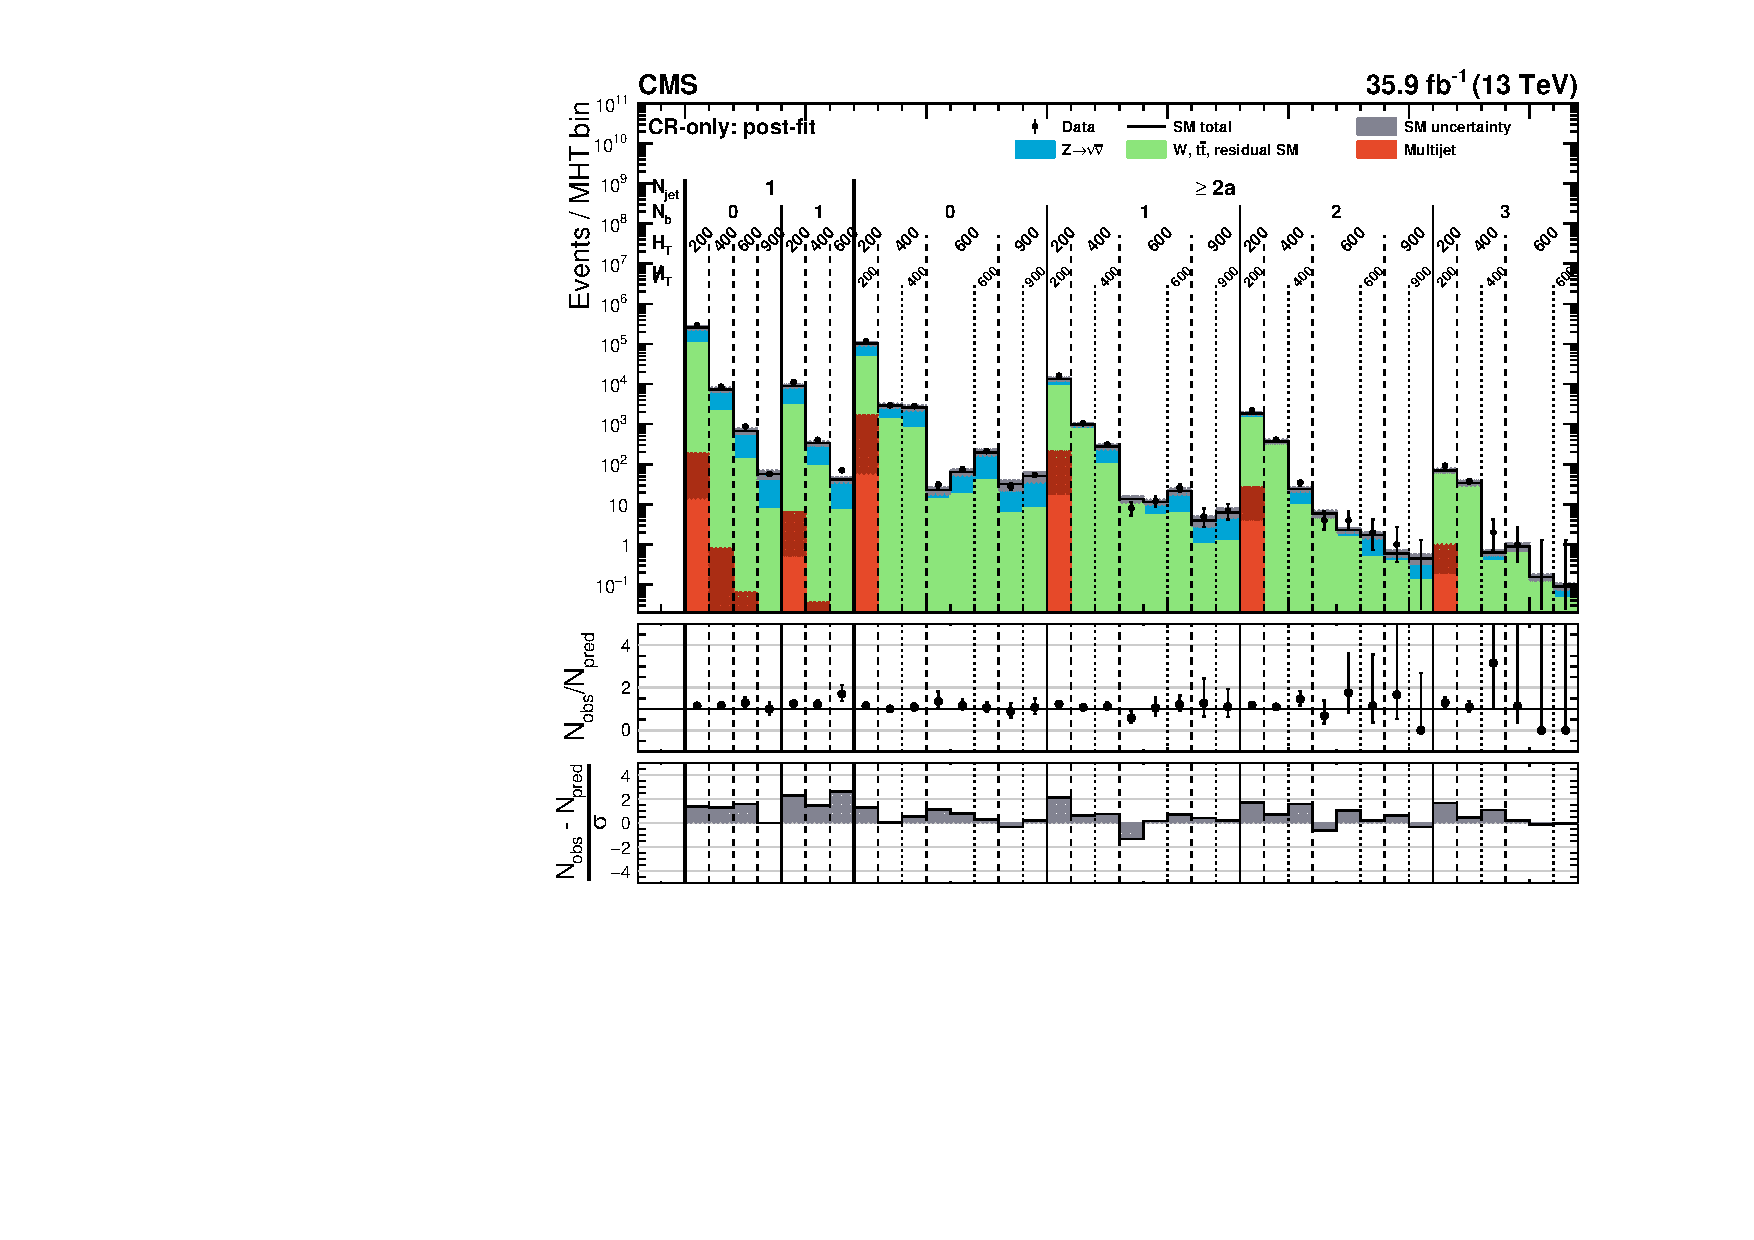
\includegraphics[width=0.48\textwidth, trim=10 0 60 10, clip=true]{Figures/1jet_cr-only.pdf}~ 
  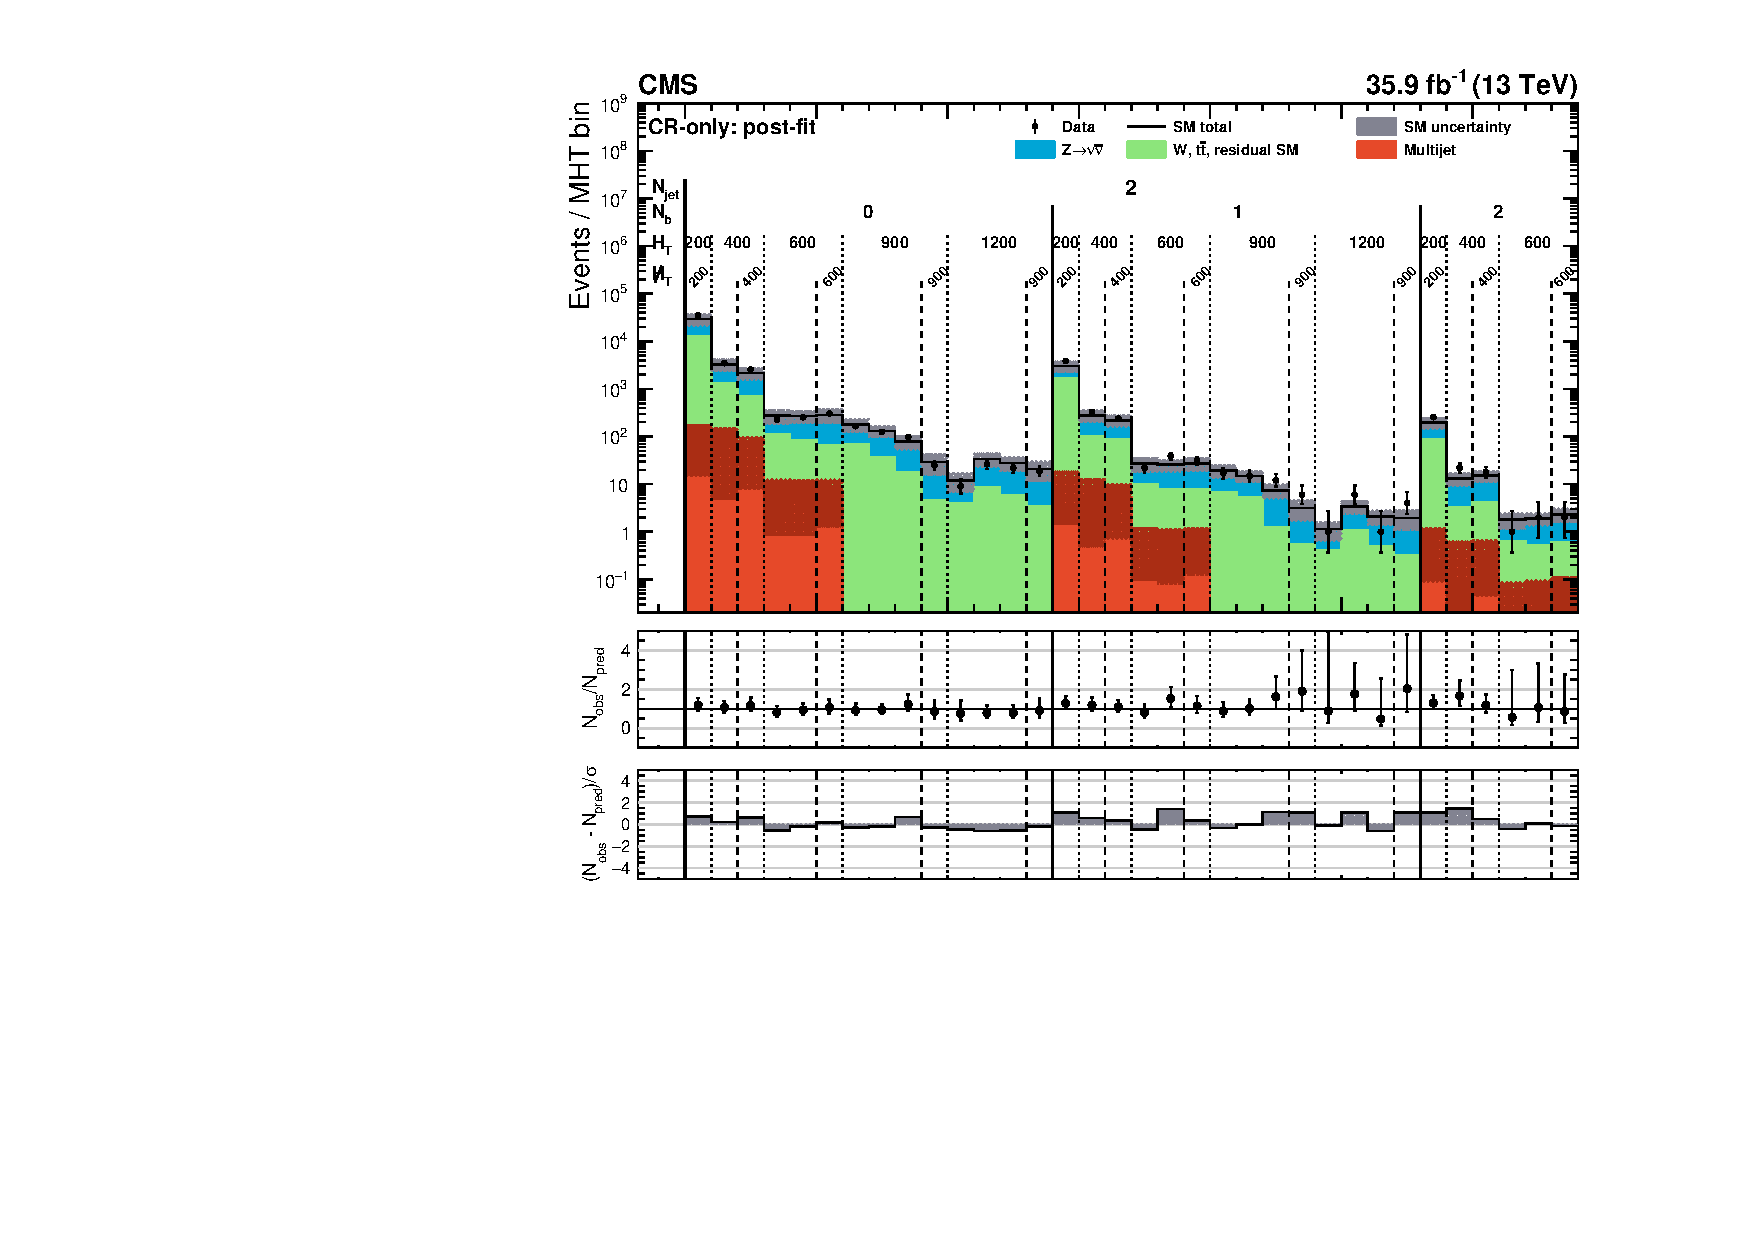
\includegraphics[width=0.48\textwidth, trim=10 0 60 10, clip=true]{Figures/2jet_cr-only.pdf}\\
  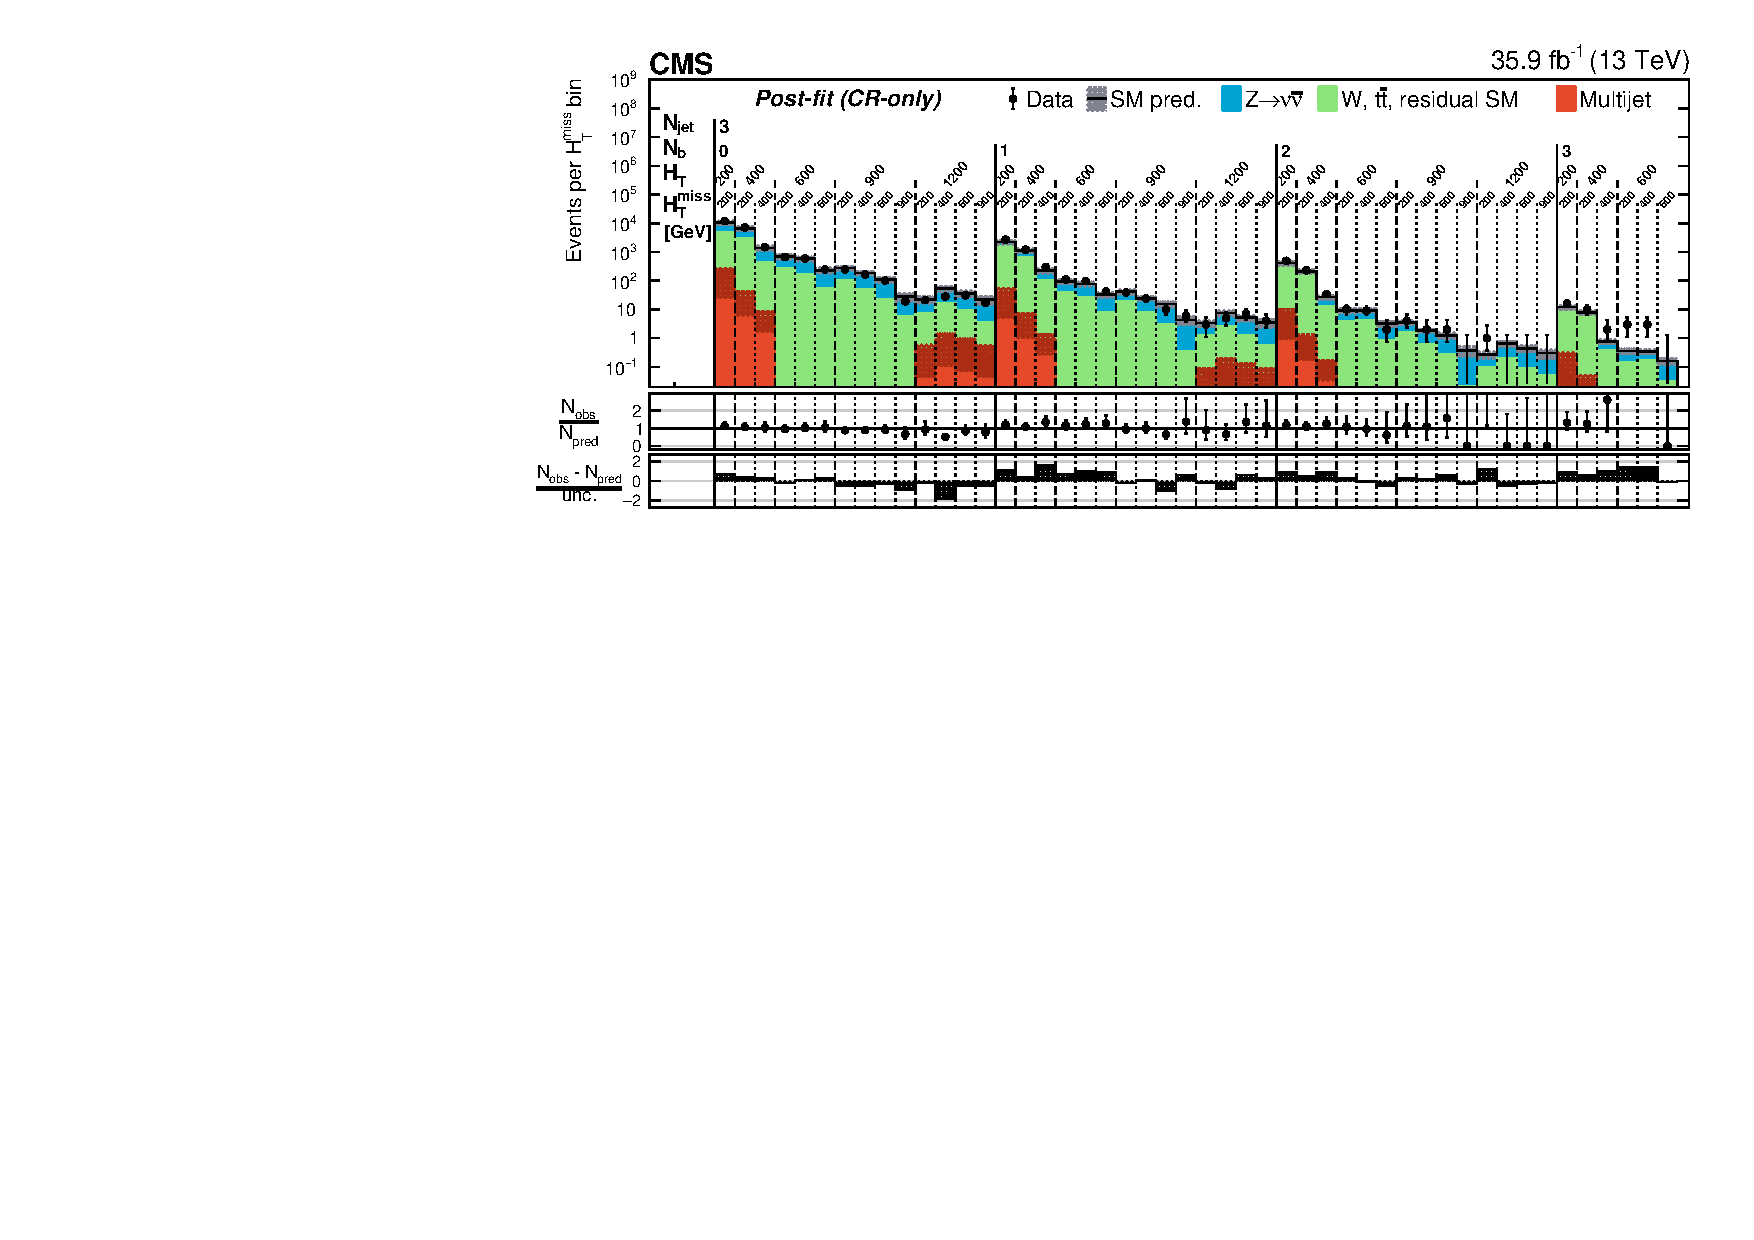
\includegraphics[width=0.48\textwidth, trim=10 0 60 10, clip=true]{Figures/3jet_cr-only.pdf}~
  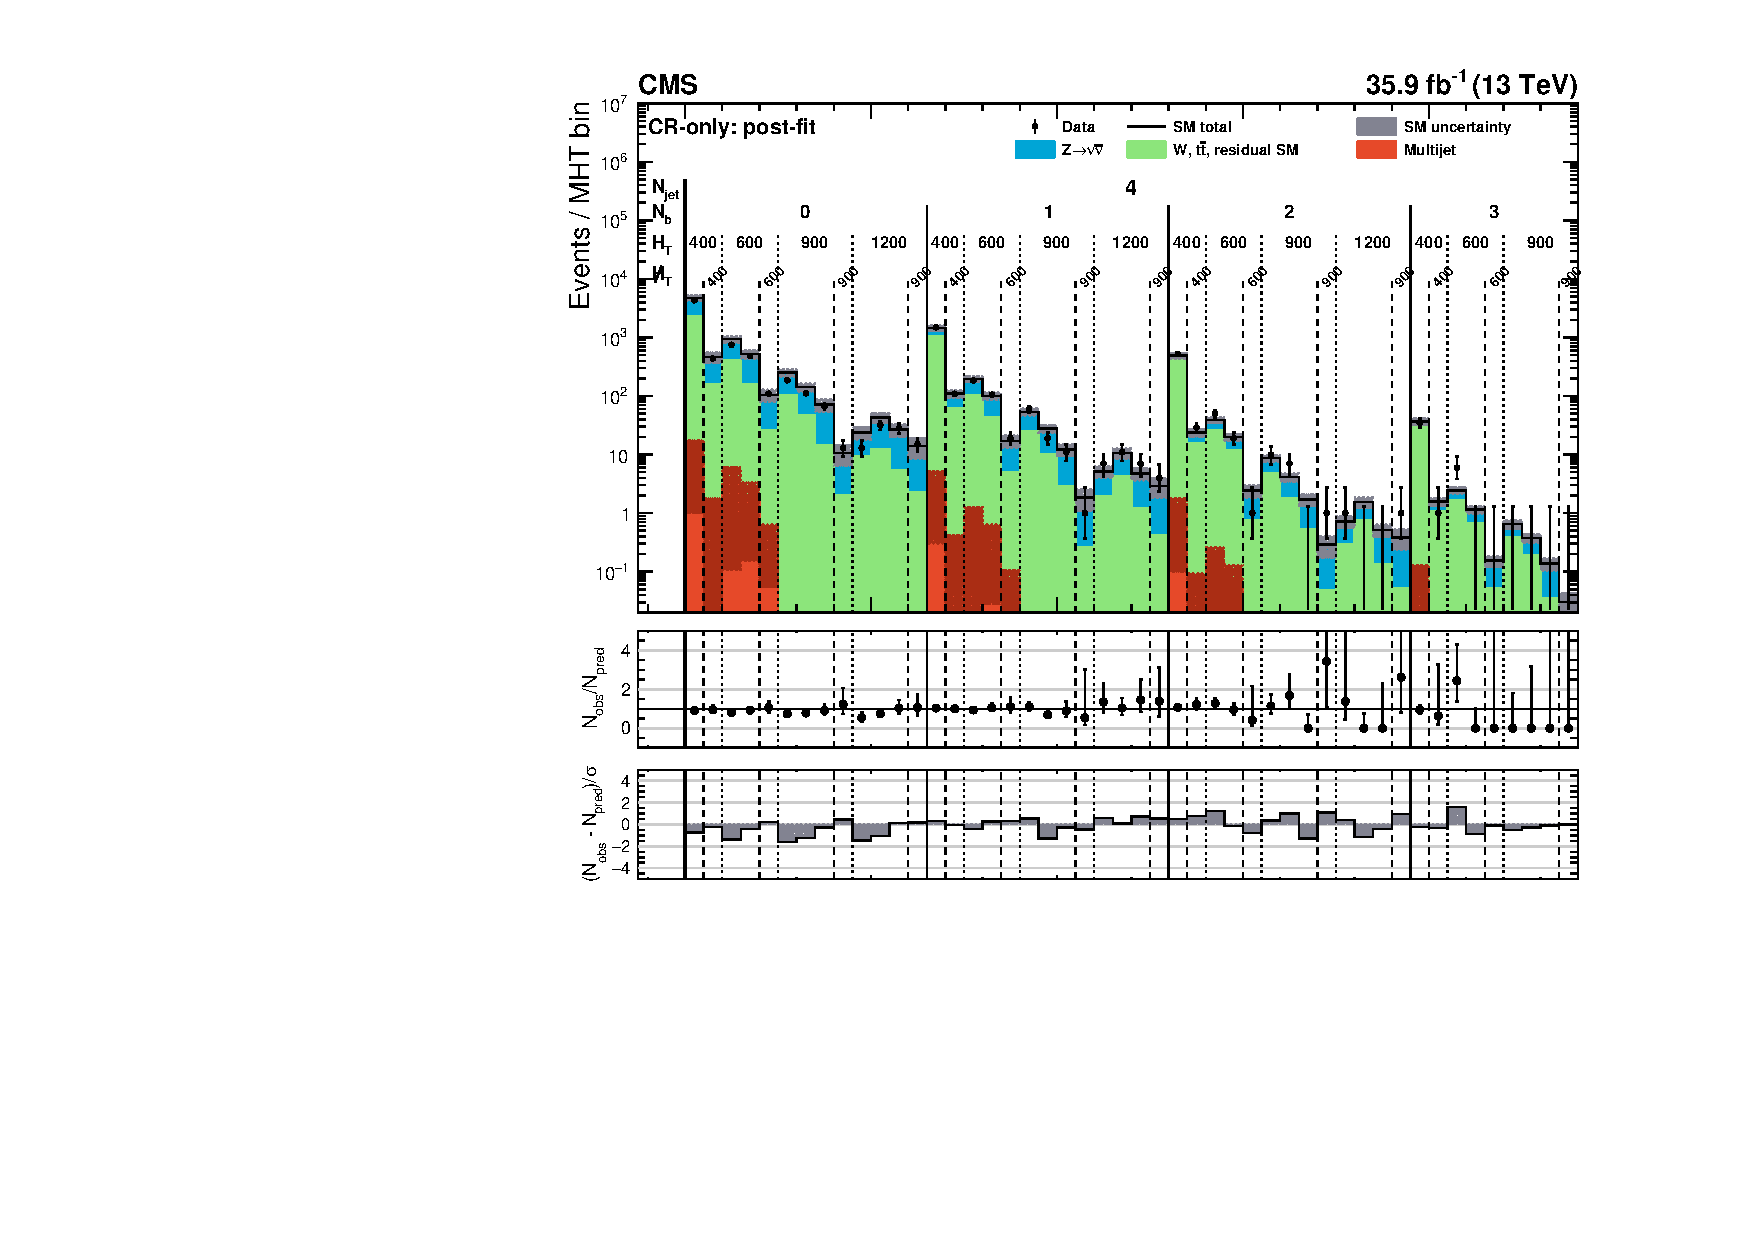
\includegraphics[width=0.48\textwidth, trim=10 0 60 10, clip=true]{Figures/4jet_cr-only.pdf}\\
  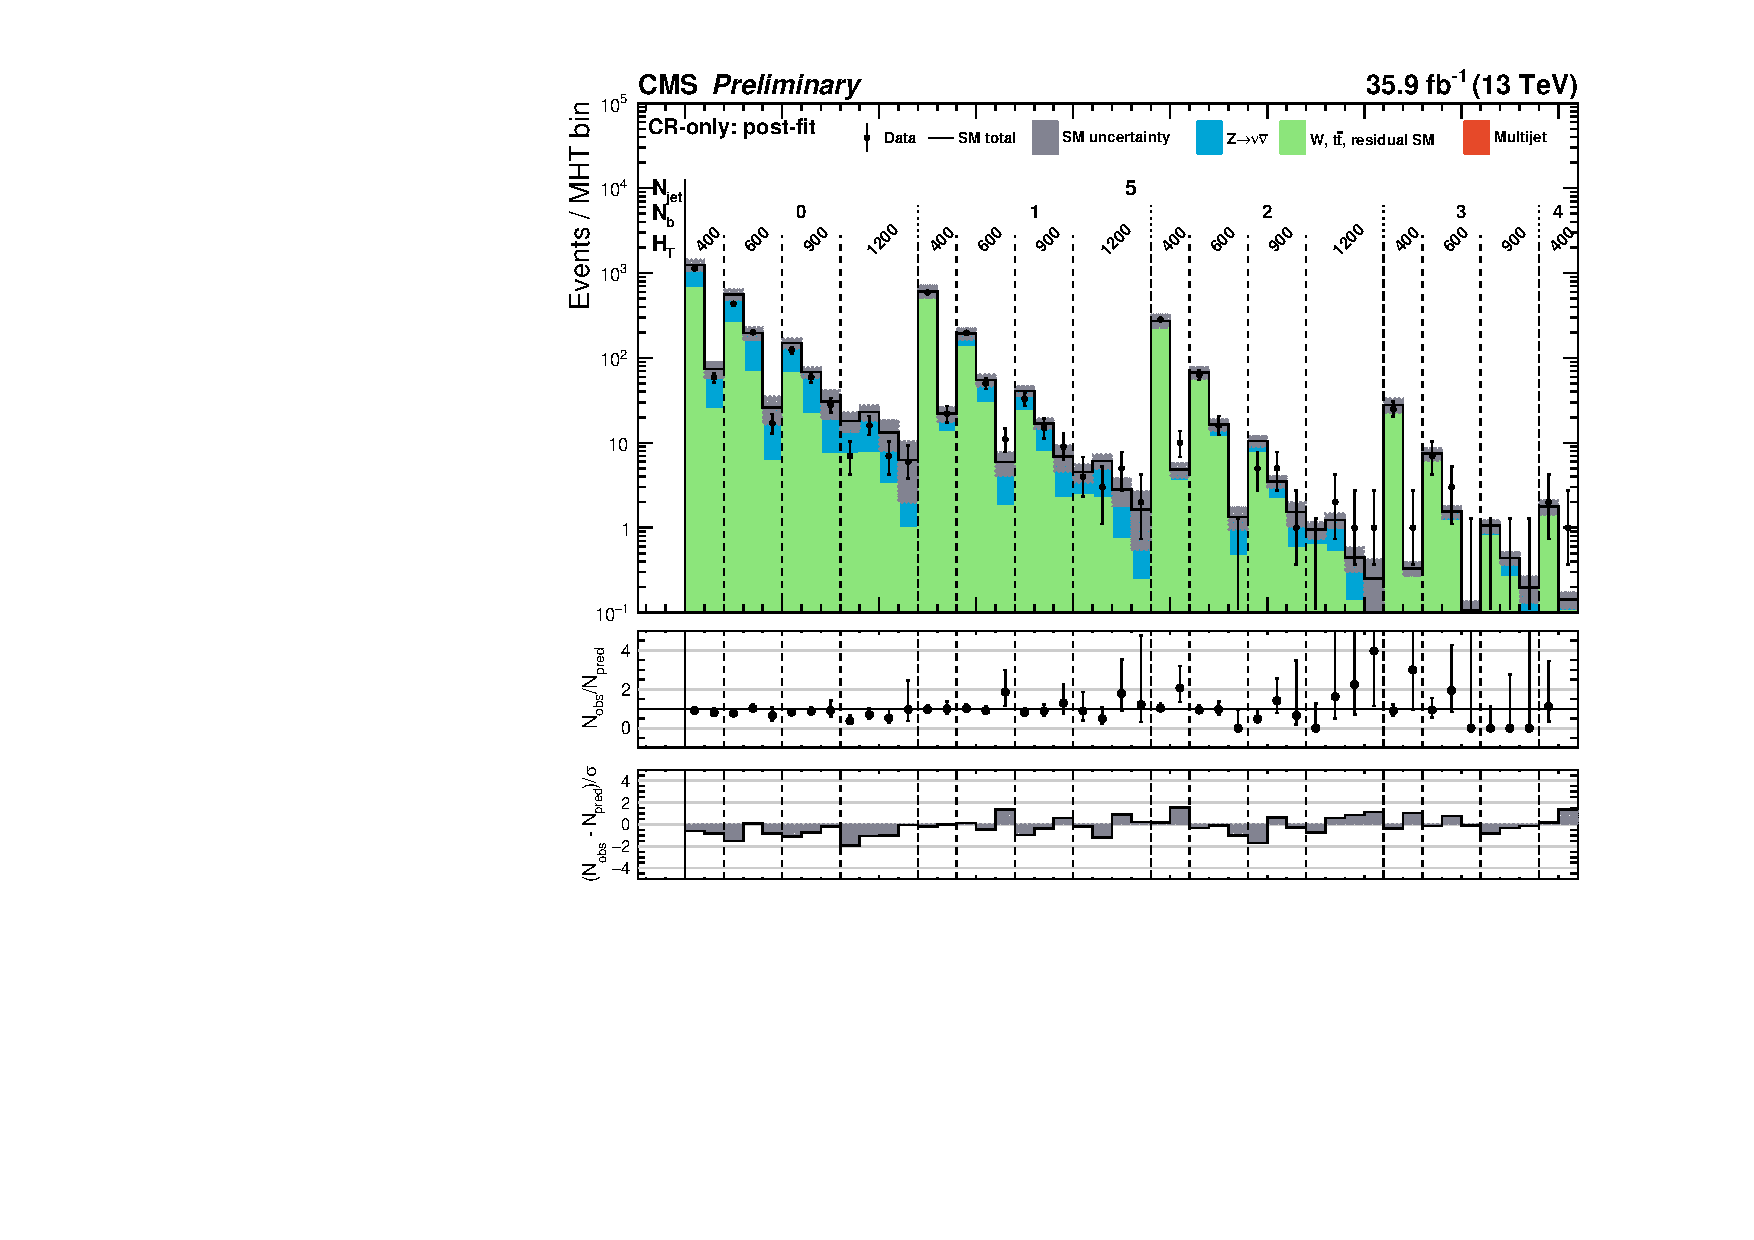
\includegraphics[width=0.48\textwidth, trim=10 0 60 10, clip=true]{Figures/5jet_cr-only.pdf}~
  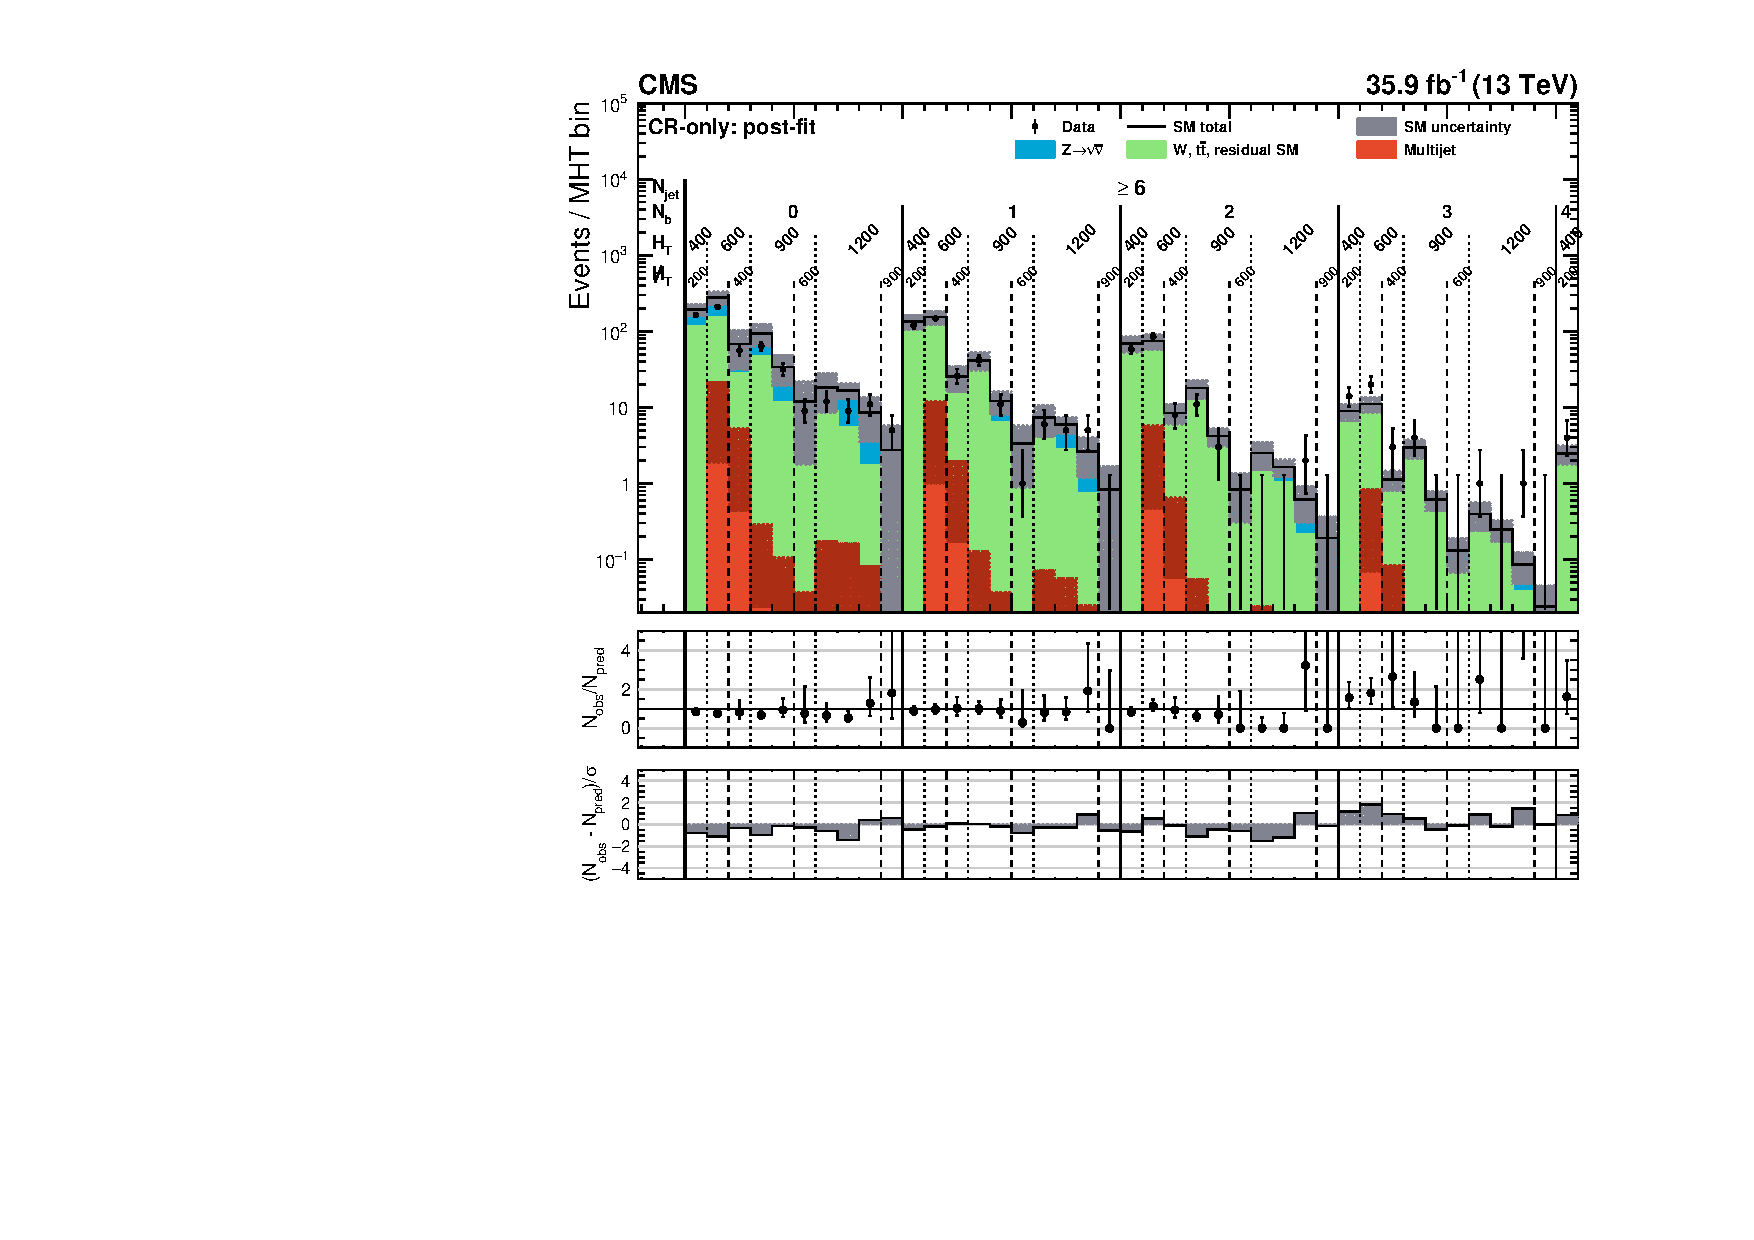
\includegraphics[width=0.48\textwidth, trim=10 0 60 10, clip=true]{Figures/6jet_cr-only.pdf}\\
  \label{fig:result}
\end{figure}

%_______________________________________________________________________________
%_______________________________________________________________________________
%_______________________________________________________________________________

%\clearpage
\section{Interpretation}
\label{sec:interpretations}

The result of the search is used to constrain the parameter space of
simplified supersymmetric models~\cite{Alwall:2008ag, Alwall:2008va,
  sms}. Each family of models realizes a unique production and decay
mode. The model parameters are the masses of the parent SUSY particle
($m_\text{SUSY}$) and neutralino ($m_\text{LSP}$). Only the
$\PSg$-mediated or direct production of top, bottom, or light-flavour
squark pairs are considered, with decays leading to final states
comprising the \chiz and SM particles. Two scenarios are considered
for light-flavoured squarks comprising $\PSQ_\cmsSymbolFace{L}$ and
$\PSQ_\cmsSymbolFace{R}$, with $\PSQ = \{\PSQu, \PSQd, \PSQs,
\PSQc\}$: one with an eightfold mass degeneracy and the other with
just a single light squark (\eg $\PSQu_\cmsSymbolFace{L}$). All other
SUSY particles are assumed to be too heavy to be produced directly. In
the case of the production of $\PSg$ pairs, three-body decays via
highly virtual squarks are assumed. In the case of decays via
light-flavour squarks, the $\PSg$ is also assumed to be metastable and
its lifetime is introduced as a third model parameter. Lifetimes in
the range $3{\times}10^{-6} < \tau < 3{\times}10^{2}\unit{ns}$ are
considered, which correpond to characteristic decay lengths in the
range $10^{-3} < c\tau < 10^{5}\unit{mm}$. Interpretations are
provided for eight unique model families, as summarised in
Table~\ref{tab:sms}.

\begingroup
\renewcommand*{\arraystretch}{1.2}
\begin{table}[!b]
  \topcaption{Summary of the simplified SUSY models used to
    interpret the result of this search.} 
  \label{tab:sms}
  \centering
  \begin{tabular}{ lll }
    \hline
    Model family
    & Production and decay
    & Additional assumptions                                                         \\
    \hline
    \multicolumn{3}{l}{\bf Production and prompt decay of $\PSg$ pairs}           \\
    \texttt{T1bbbb}
    & $\Pp\Pp \to \PSg\PSg$,
    $\PSg\to \cPaqb\PSQb^* \to \cPaqb\cPqb\PSGczDo$
    & $m_{\PSQb} \gg m_{\PSg}$                                                       \\
    \texttt{T1tttt}
    & $\Pp\Pp \to \PSg\PSg$,
    $\PSg\to \cPaqt\PSQt^* \to \cPaqt\cPqt\PSGczDo$                                                                   
    & $m_{\PSQt} \gg m_{\PSg}$                                                       \\
    \multicolumn{3}{l}{\bf Production and prompt decay of squark pairs}           \\
    \texttt{T2bb}
    & $\Pp\Pp \to \PSQb\PASQb$,
    $\PSQb \to \cPqb\PSGczDo$
    & --                                                                             \\
    \texttt{T2tt}
    & $\Pp\Pp \to \PSQt\PASQt$,
    $\PSQt \to \cPqt\PSGczDo$
    & --                                                                             \\
    \texttt{T2cc}
    & $\Pp\Pp \to \PSQt\PASQt$,
    $\PSQt\to \cPqc\PSGczDo$
    & $10 < m_{\,\PSQt} - m_{\PSGczDo} < 80\GeV$                                     \\
    \texttt{T2qq\_8fold}
    & $\Pp\Pp \to \PSQ\PASQ$,
    $\PSQ \to \cPq\PSGczDo$
    & $m_{\PSQ_\cmsSymbolFace{L}} = m_{\PSQ_\cmsSymbolFace{R}}$,
    $\PSQ = \{ \PSQu, \PSQd, \PSQs, \PSQc \}$                                     \\
    \texttt{Tqq\_1fold}
    & $\Pp\Pp \to \PSQ\PASQ$,
    $\PSQ \to \cPq\PSGczDo$
    & $m_{\PSQ (\PSQ \neq \PSQu_\cmsSymbolFace{L})} \gg m_{\PSQu_\cmsSymbolFace{L}}$ \\
    \multicolumn{3}{l}{\bf Production and decay of long-lived $\PSg$ pairs}       \\
    \texttt{T1qqqqLL}
    & $\Pp\Pp \to \PSg\PSg$,
    $\PSg \to \cPaq\PSQ^* \to \cPaq\cPq\PSGczDo$    
    & $m_{\PSQ} \gg m_{\PSg}$, $10^{-3} < c\tau < 10^{5}\unit{mm}$                   \\
    \hline
  \end{tabular}
\end{table}
\endgroup 

Under the signal+background hypothesis, and in the presence of a
nonzero signal contribution, a modified frequentist approach is used
to determine observed upper limits at 95\% confidence level (CL) on
the cross section $\sigma_\text{UL}$ to produce pairs of SUSY
particles as a function of $m_\text{SUSY}$, $m_\text{LSP}$, and
$c\tau$ (if applicable). The approach is based on the aforementioned
profile likelihood ratio as the test statistic, the \cls
criterion~\cite{junk, read}, and asymptotic
formulae~\cite{Cowan:2010js} to approximate the distributions of the
test statistic under the SM-background-only and signal+background
hypotheses.  An Asimov data set~\cite{Cowan:2010js} is used to
determine the expected $\sigma_\text{UL}$ on the allowed cross section
for a given model. Potential signal contributions to event counts in
all bins of the SR and CRs are considered.%, even though the only
%significant contribution occurs in the SR. 

The experimental acceptance times efficiency ($\mathcal{A} \times
\varepsilon$) and is evaluated independently for each model, defined
in terms of $m_\text{SUSY}$, $m_\text{LSP}$, and $c\tau$ (if
applicable). Several sources of uncertainty in $\mathcal{A} \times
\varepsilon$ are considered. The effects of several sources of
uncertainty in $\mathcal{A} \times \varepsilon$, as well as the
potential for migration of events between bins of the SR, are
considered. Correlations are taken into account where appropriate,
including those relevant to signal contamination that may contribute
to counts in the CRs. The magnitude of each source of uncertainty is
dependent on the model and its parameters.

One or more of the following sources of uncertainty typically dominate
in a region of the model parameter space. The statistical uncertainty
arising from the finite size of simulated samples can be as large as
${\approx}30\%$. The $\mathcal{A} \times \varepsilon$ for models with
small mass splittings (\ie the regime $m_{\PSQ} - m_{\PSGczDo}
\lesssim 200\GeV$) relies somewhat on jets arising from ISR, the
modelling of which is evaluated by comparing the simulated and
measured \pt spectra of the system recoiling against the ISR jets in
\ttbar events, using the technique described in
Ref.~\cite{single-lepton-stop}. The uncertainty can be as large as
${\approx}30\%$ for near mass-degenerate systems. The corrections to
the jet energy scale evaluated with simulated events can lead to
variations in event counts as large as ${\approx}25\%$ for models
characterised by high jet multiplicities in the final state. The
uncertainties in the modelling of scale factors applied to simulated
event samples that correct for differences in the b-tag efficiency
($\text{SF}_\text{b}$) and mistag probability of light-flavour partons
and charm quarks ($\text{SF}_\text{LF}$), evaluated independently, can
be as large as ${\approx}20$ and ${\approx}X\%$, respectively.

\begingroup
\renewcommand*{\arraystretch}{1.1}
\begin{table}[!t]
  \topcaption{A list of benchmark simplified models organised
    according to production and decay modes (family), %a representative
    %(\njet, \nb) topology that indicates a sensitive region for each
    %model, 
    the $\mathcal{A} \times \varepsilon$, %this topology, 
    representative values for some of the dominant sources of 
    systematic uncertainty, and the expected and observed upper limits
    on the production cross section, expressed in terms of the signal
    strength parameter ($\mu$). Additional uncertainties concerning
    the \texttt{T1qqqqLL} models are not listed here and are discussed
    in the text.   
  }
  \label{tab:benchmarks}
  \centering
  \resizebox{\textwidth}{!}{
    \begin{tabular}{ lrcrrrrrrcc }
      \hline
      Family
      & $(m_{\text{SUSY}}, m_{\mathrm{LSP}})$
      %& Sensitive%(\njet, \nb)
      & $\mathcal{A} \times \varepsilon$
      & \multicolumn{5}{c}{Systematic uncertainties [\%]}
      & \multicolumn{2}{c}{$\mu$ (95\% CL)}                                                                            \\ [0.3ex]
      \cline{4-8}
      ($c\tau$)
      & [\GeVns{}]
      %& topology
      & [\%]
      & MC stat.
      & ISR
      & JEC
      & $\text{SF}_\text{b}$
      & $\text{SF}_\text{LF}$
      & Exp.
      & Obs.                                                                                                           \\ [0.3ex]
      \hline
      \multirow{2}{*}{\texttt{T1bbbb}}
      & (1900, 100)  %& (${\geq}6, {\geq}2$)  
      & 25.1           & 11--19 & 3--9   & 4--6   & 7--12 & --    & 0.56 & 1.25 \\
      & (1300, 1100) %& (${\geq}6, {\geq}2$)  
      & 14.6           & 11--22 & 2--11  & 3--11  & 2--5  & --    & 0.44 & 1.15 \\ [0.5ex]
      \multirow{2}{*}{\texttt{T1tttt}}
      & (1700, 100)  %& (${\geq}6, {\geq}2$)  
      & \phantom{1}6.9 & 12--24 & 2--6   & 3--15  & 2--6  & --    & 0.51 & 1.31 \\
      & (950, 600)   %& (${\geq}6, {\geq}2$)  
      & \phantom{1}0.3 & 15--30 & 5--9   & 12--26 & 2--6  & --    & 0.89 & 1.51 \\ [0.5ex]
      \multirow{2}{*}{\texttt{T2bb}}
      & (800, 50)    %& (${\geq}6, {\geq}2$)  
      & 40.1           & 14--23 & 1--7   & 4--11  & 1--4  & --    & 0.62 & 0.67 \\
      & (375, 300)   %& (${\geq}6, {\geq}2$)  
      & \phantom{1}5.7 & 9--22  & 4--15  & 4--15  & 3--7  & --    & 0.76 & 1.21 \\ [0.5ex]
      \multirow{3}{*}{\texttt{T2tt}}
      & (1000, 50)   %& (${\geq}6, {\geq}2$)  
      & 23.8           & 14--27 & 3--7   & 4--14  & 1--5  & --    & 0.82 & 0.85 \\
      & (450, 200)   %& (${\geq}6, {\geq}2$)  
      & \phantom{1}4.2 & 6--19  & 4--12  & 6--15  & 4--9  & --    & 0.56 & 0.73 \\ [0.5ex]
      & (250, 150)   %& (${\geq}6, {\geq}2$)  
      & \phantom{1}0.3 & 10--23 & 13--27 & 8--22  & 6--16 & --    & 0.71 & 0.66 \\ [0.5ex]
      \multirow{1}{*}{\texttt{T2cc}}
      & (500, 480)   %& (${\geq}6, {\geq}2$)  
      & 20.5           & 6--19  & 4--18  & 5--13  & 1--4  & --    & 0.68 & 1.38 \\ [0.5ex]
      \multirow{2}{*}{\texttt{T2qq\_8fold}}
      & (1250, 100)  %& (${\geq}6, {\geq}2$)  
      & 42.9           & 12--24 & 2--7   & 5--14  & 1--1  & --    & 0.54 & 0.66 \\
      & (700, 600)   %& (${\geq}6, {\geq}2$)  
      & \ph{1}7.7      & 6--22  & 4--17  & 4--13  & 2--5  & --    & 0.75 & 1.13 \\ [0.5ex]
      \multirow{2}{*}{\texttt{T2qq\_1fold}}
      & (700, 100)   %& (${\geq}6, {\geq}2$)  
      & 32.9           & 4--22  & 2--7   & 3--10  & 0--5  & --    & 0.60 & 0.88 \\
      & (400, 300)   %& (${\geq}6, {\geq}2$)  
      & \ph{1}4.5      & 6--20  & 5--22  & 5--18  & 3--5  & --    & 0.61 & 0.46 \\ [0.5ex]
      \texttt{T1qqqqLL}
      & (1800, 200)  %& (${\geq}6, {\leq}1$)  
      & 27.8           & 8--16  & 3--5   & --     & 0--1  & 2--9  & 0.81 & 1.58 \\
      ($10^{-3}\unit{mm}$)
      & (1000, 900)  %& (${\leq}2a, {\leq}1$) 
      & \ph{1}6.7      & 13--24 & 1--12  & --     & 0--1  & 0--1  & 0.95 & 1.21 \\ [0.5ex]
      \texttt{T1qqqqLL}
      & (1800, 200)  %& (${\geq}6, {\geq}2$)  
      & 22.9           & 17--22 & 2--4   & --     & 3--16 & 3--14 & 0.36 & 0.66 \\
      ($10^{0}\unit{mm}$)
      & (1000, 900)  %& (${\leq}2a, {\leq}1$) 
      & \ph{1}5.2      & 20--29 & 3--9   & --     & 4--9  & 8--13 & --   & --   \\ [0.5ex]
      \texttt{T1qqqqLL}
      & (1000, 200)  %& (4--5, ${\leq}1$)     
      & 11.2           & 16--30 & 2--17  & --     & 0--1  & 1--1  & 0.95 & 1.33 \\
      ($10^{5}\unit{mm}$)
      & (1000, 900)  %& (${\leq}2a, {\leq}1$) 
      & 10.4           & 14--25 & 3--14  & --     & 0--1  & 1--1  & --   & 0.73 \\ [0.5ex]
%      \\
%      \texttt{T1qqqqLL}
%      & (1800, 200)  & (${\geq}6, {\leq}1$)  & \ph{1}0.1                                                               \\
%      & (1000, 900)  & (${\leq}2a, {\leq}1$) & \ph{1}0.5                                                               \\
%      \texttt{T1qqqqLL}
%      & (1800, 200)  & (${\geq}4, {\geq}2$)  & \ph{1}0.1                                                               \\
%      & (1000, 900)  & (${\leq}2a, {\leq}1$) & \ph{1}0.6                                                               \\
%      \texttt{T1qqqqLL}
%      & (1000, 200)  & (4--5, ${\leq}1$)     & \ph{1}0.5                                                               \\
%      & (1000, 900)  & (${\leq}2a, {\leq}1$) & \ph{1}0.6                                                               \\
      \hline
    \end{tabular}
  }
\end{table}
\endgroup

Table~\ref{tab:benchmarks} defines a number of benchmark models that
are at the limit of the search sensitivity, which are used to develop
an understanding of the expected parameter-space coverage. All
families (of production and decay modes) are represented, and the
model parameters ($m_\text{SUSY}$, $m_\text{LSP}$, and $c\tau$ if
applicable) are chosen to select models with large and small mass
differences, as well as prompt-like, b-quark-like, and stable-like
decay lengths. Table~\ref{tab:benchmarks} summarises the
aforementioned uncertainties for each benchmark model, presented in
terms of a characteristic range that is representative of the
variations observed across the bins of the SR. The upper bound for
each range may be subject to moderate statistical fluctuations.

Additional subdominant contributions to the total uncertainty are also
considered. The uncertainty in the integrated luminosity is determined
to be 2.5\%~\cite{CMS:2017sdi}. Uncertainties in $\sigma_\text{prod}$
arising from the choice of PDF set, and variations therein, as well as
variations in the renormalisation and factorisation scales
($\mu_\text{R}$ and $\mu_\text{F}$) at LO are
considered. Uncertainties in event migration between bins from
variations in the PDF sets are assumed to be correlated with, and
adequately covered by, the uncertainties in the modelling of
ISR. Uncertainties from $\mu_\text{R}$ and $\mu_\text{F}$ variations
are determined to be ${\approx}5\%$. The effect of a 5\% uncertainty
in the total inelastic cross section~\cite{Aaboud:2016mmw} is
propagated through the reweighting procedure that corrects for
differences between the simulated and measured pileup, resulting in
event-count variations of ${\approx}10\%$. Uncertainty in the
modelling of the efficiency to identify high-quality, isolated leptons
is ${\approx}5\%$ and is treated as anticorrelated between the SR and
\mj and \mmj CRs. The uncertainty in the trigger efficiency to record
candidate signal events is $<$10\%.

% Finally, the efficiency of reconstructing jets with displaced
% vertices resulting from the decay of long-lived $\PSg$ particles, as
% well as the probability of tagging these displaced jets as arising
% from b quarks, are inspected as a function of the displacement. BLAH
% ... Additional uncertainties associated with these quantities are
% assigned BLAH ...

Figure~\ref{fig:limits} summarises the excluded regions of the
mass parameter space for seven families of simplified model. The
regions are determined by comparing the upper limits on the measured
fiducial cross section, corrected for the experimental
$\mathcal{A}\,\varepsilon$, with the theoretical cross sections
calculated at NLO+NLL accuracy in
$\alpha_\mathrm{s}$~\cite{susynlo}. The former cross section value is
determined as a function of $m_{\PSg}$ or $m_{\PSQ}$ and
$m_{\PSGczDo}$, while the latter has a dependence solely on $m_{\PSg}$
or $m_{\PSQ}$.  The exclusion of models is evaluated using observed
data counts in the signal region (solid contours) and also expected
counts based on an Asimov data set (dashed contours).

%All these models assume the prompt decay of the parent SUSY particle.
%
%fourteen classes of simplified
%models. 
%
%Figure~\ref{fig:limits-sms} shows the observed values of
%$\sigma_\text{UL}$ as a function of the $\PSg$ or squark and \chiz
%masses for the \texttt{T1bbbb} and \texttt{T1tttt} model
%families. Also shown are the observed excluded regions of the mass
%parameter space when varying the production cross section by its
%theoretical uncertainty, and the expected mass exclusion regions with
%the ${\pm}1$ and ${\pm}2$ standard-deviation variations.
%
%The search places stringent limits in the mass parameter space of
%these models, with observed exclusions in $\PSg$ and \chiz masses as
%high as 1900 and 1175\GeV, respectively. In the case of direct
%production of bottom squarks, masses as high as 1075 and 535\GeV are
%excluded. Finally, top squark and \chiz masses up to 1040 and 580\GeV
%are excluded. 

\begin{figure}[!t]
  \centering
  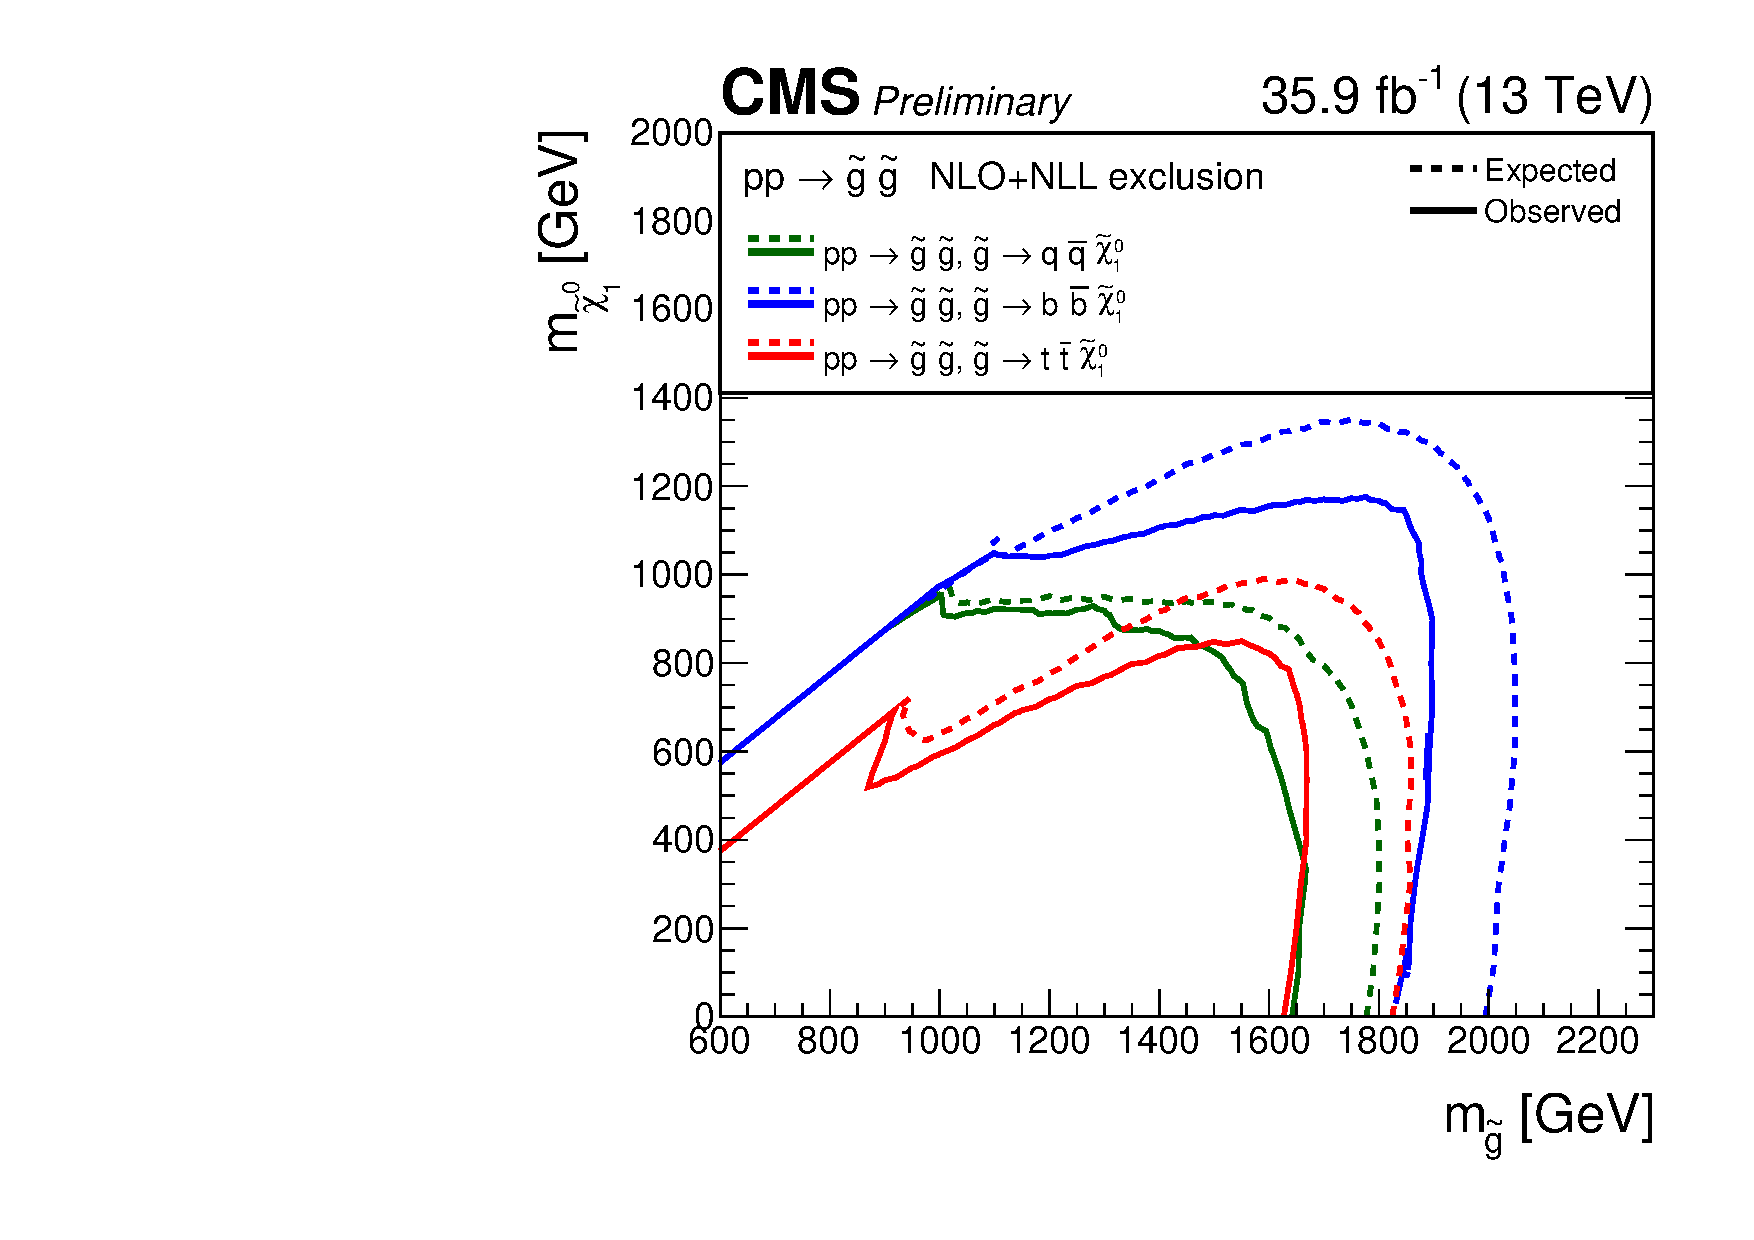
\includegraphics[width=0.49\textwidth]{Figures/gluinoSUMMARY.pdf}~
  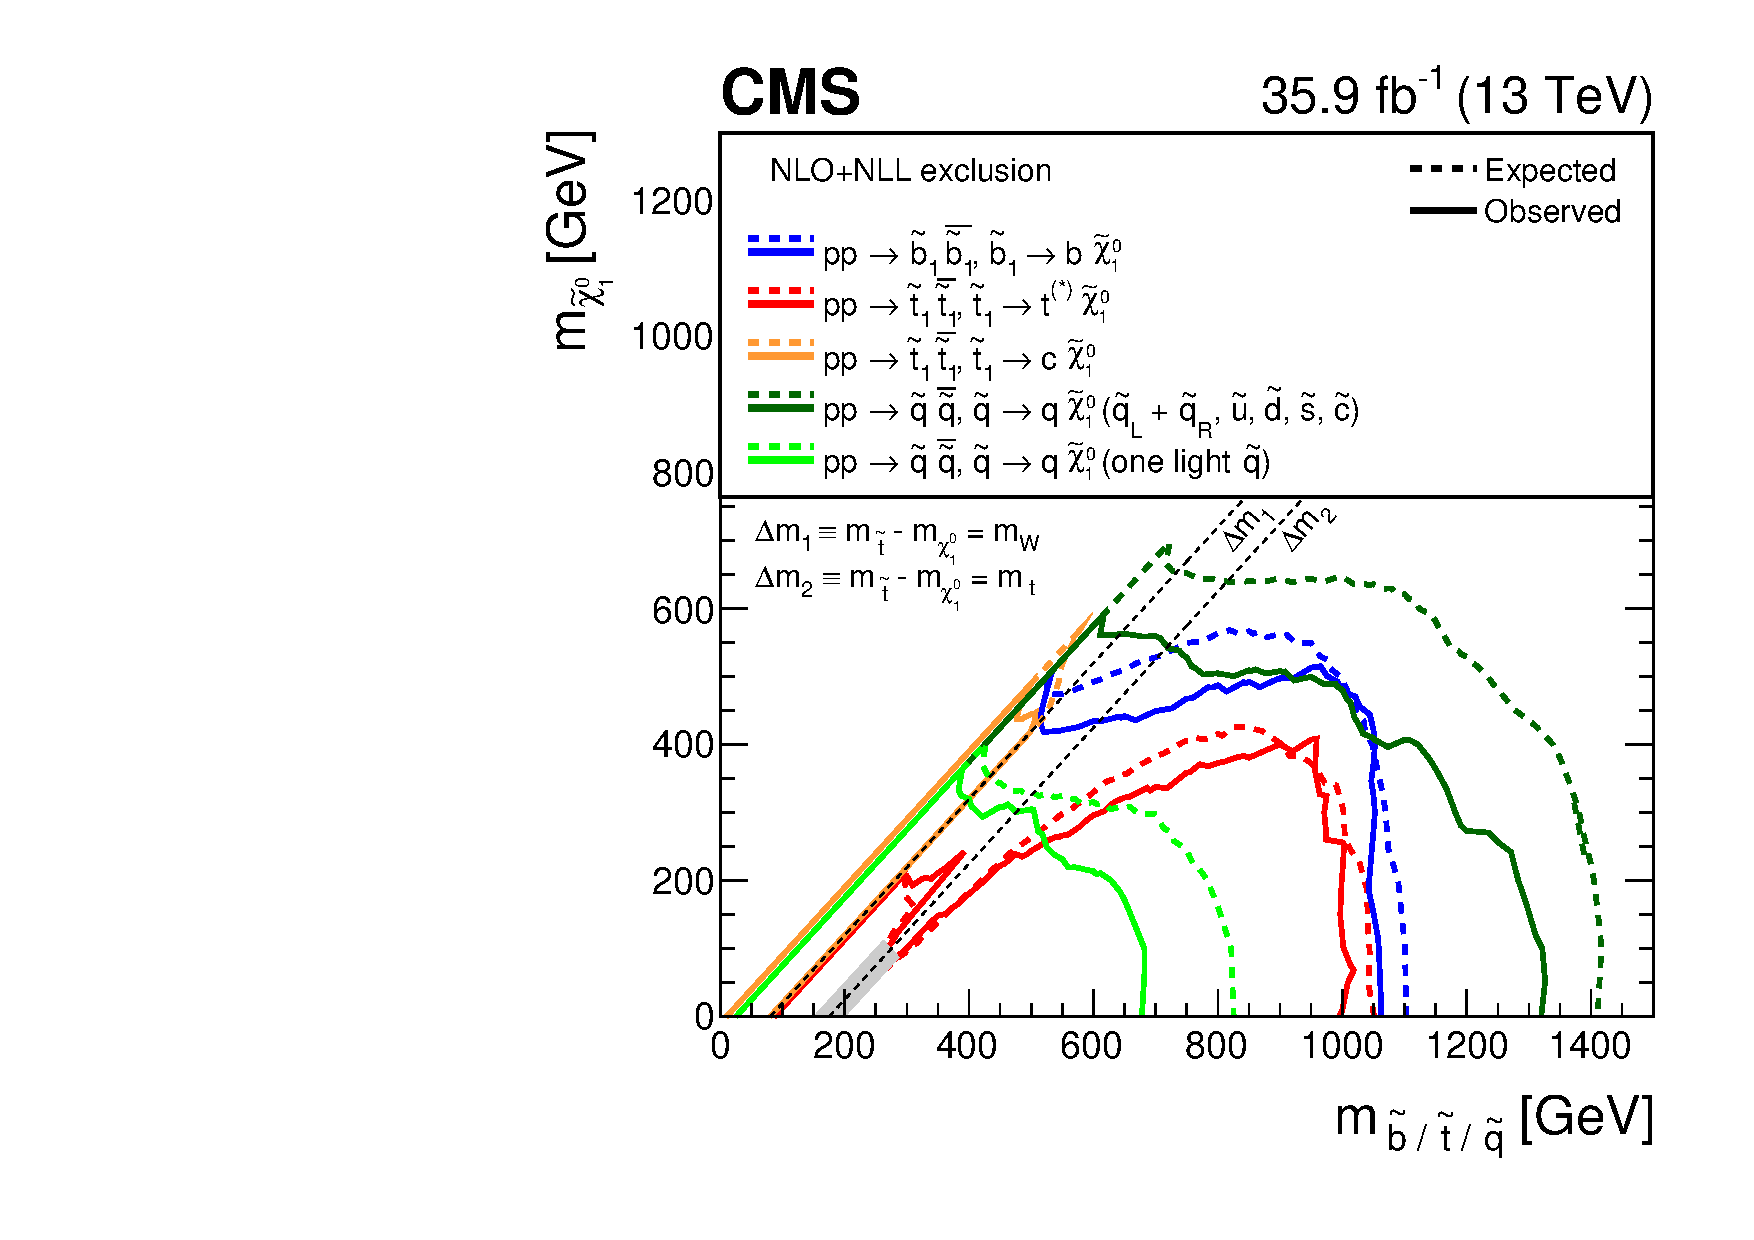
\includegraphics[width=0.49\textwidth]{Figures/squarkSUMMARY.pdf}\\
  \caption{Observed and expected mass exclusions at 95\% CL
    (indicated, respectively, by solid and dashed contours) for
    various families of simplified models. (\cmsLeft) $\PSg$-mediated
    pair production of off-shell third-generation squarks: $\PSg\to
    \cPaqb\cPqb\PSGczDo$ (\texttt{T1bbbb}) and $\PSg\to
    \cPaqt\PSQt^*\to \cPaqt\cPqt\PSGczDo$ (\texttt{T1tttt}).
    (\cmsRight) Five model families involving the direct pair
    production of squarks. The first two scenarios involve,
    respectively, the production and decay of light-flavour squarks,
    $\PSQ\to \cPq\PSGczDo$, with different assumptions on the mass
    degeneracy of the squarks as described in the text
    (\texttt{T2qq\_8fold} and \texttt{T2qq\_1fold}). A further
    scenario considers the pair production and decay of bottom
    squarks, $\PSQb\to \cPqb\PSGczDo$ (\texttt{T2bb}). Finally, two
    scenarios involve the production and decay of top squark pairs as
    follows: $\PSQt\to \cPqt\PSGczDo$ (\texttt{T2tt}) and $\PSQt\to
    \cPqc\PSGczDo$ (\texttt{T2cc}). The grey shaded region denotes
    \texttt{T2tt} models that are not considered for interpretation.
  }
  \label{fig:limits} 
\end{figure}

\clearpage
\begin{figure}[!t]
  \centering
  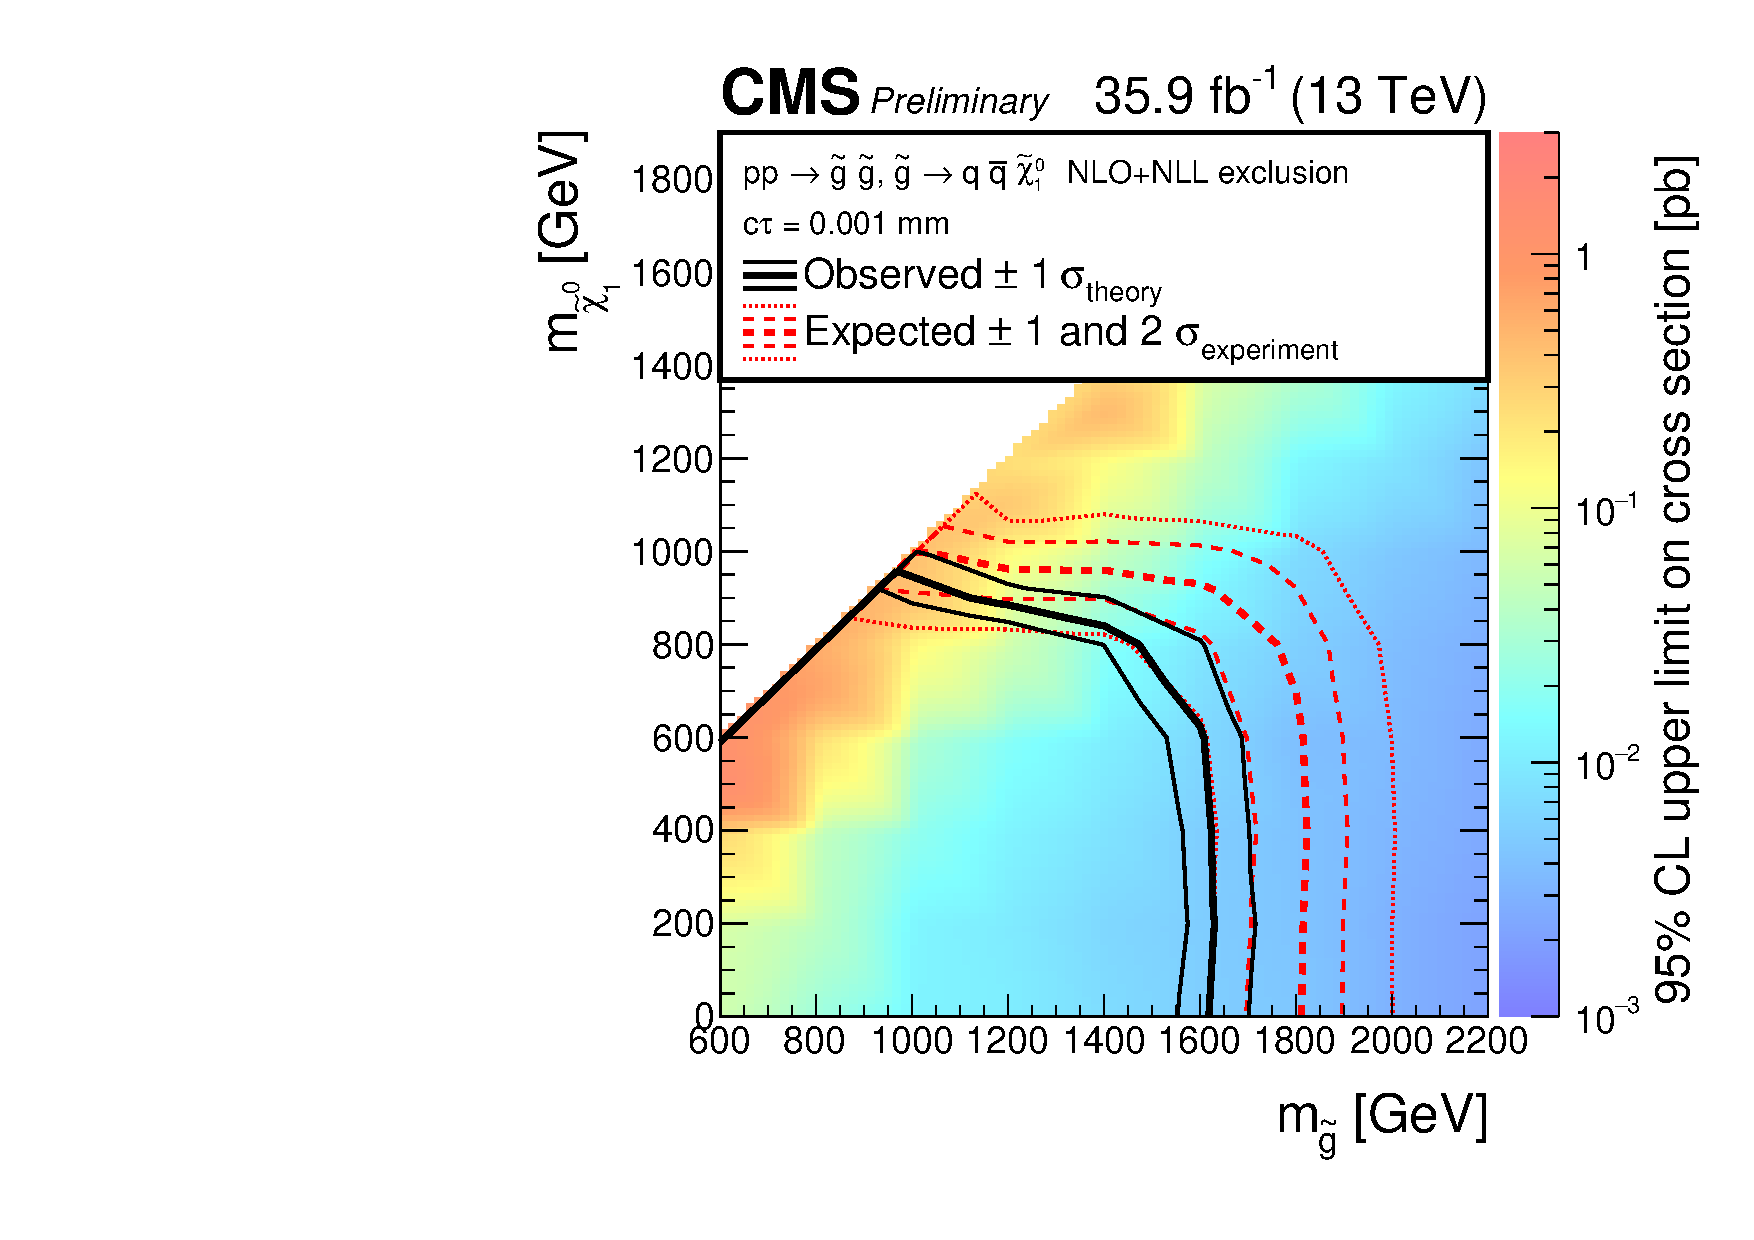
\includegraphics[width=0.33\textwidth]{Figures/T1qqqqLL_ctau-0p001_XSEC}~
  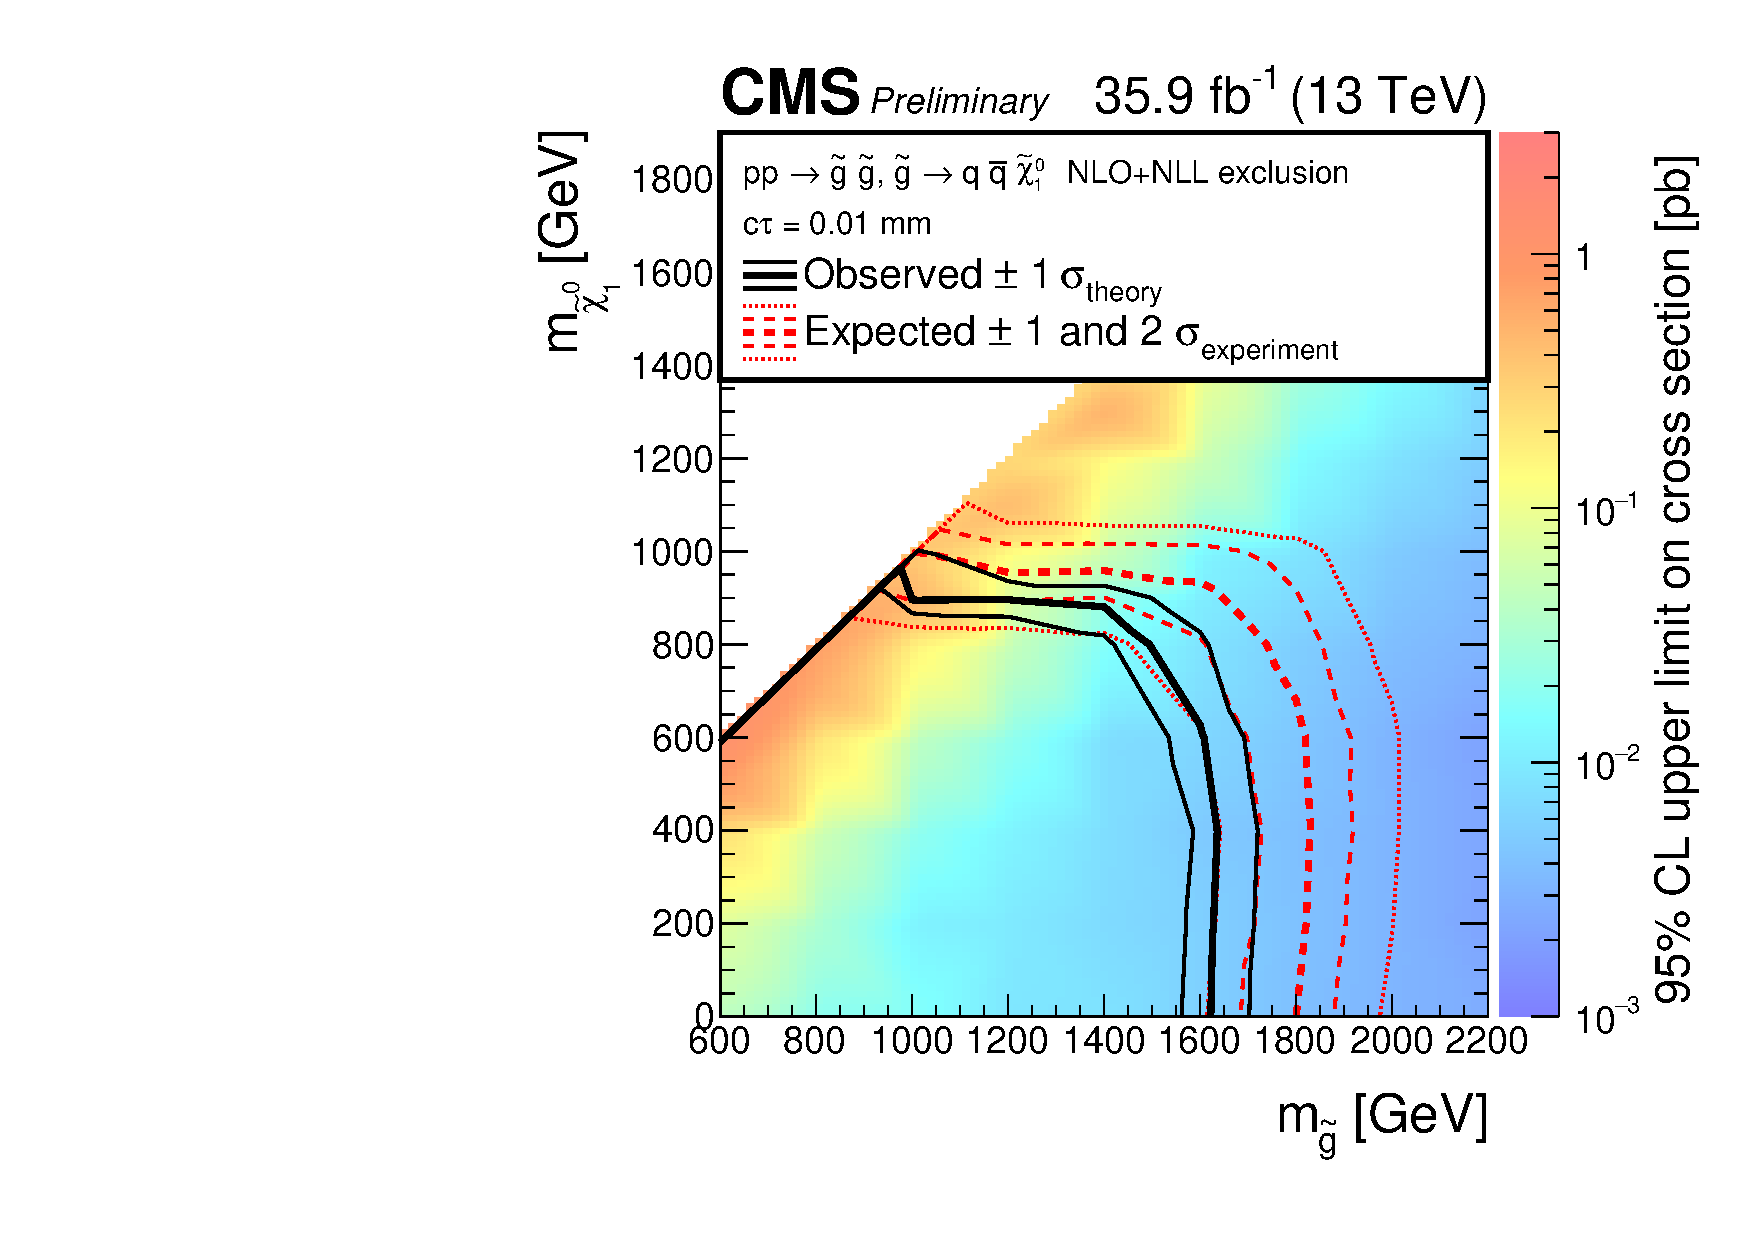
\includegraphics[width=0.33\textwidth]{Figures/T1qqqqLL_ctau-0p01_XSEC}~
  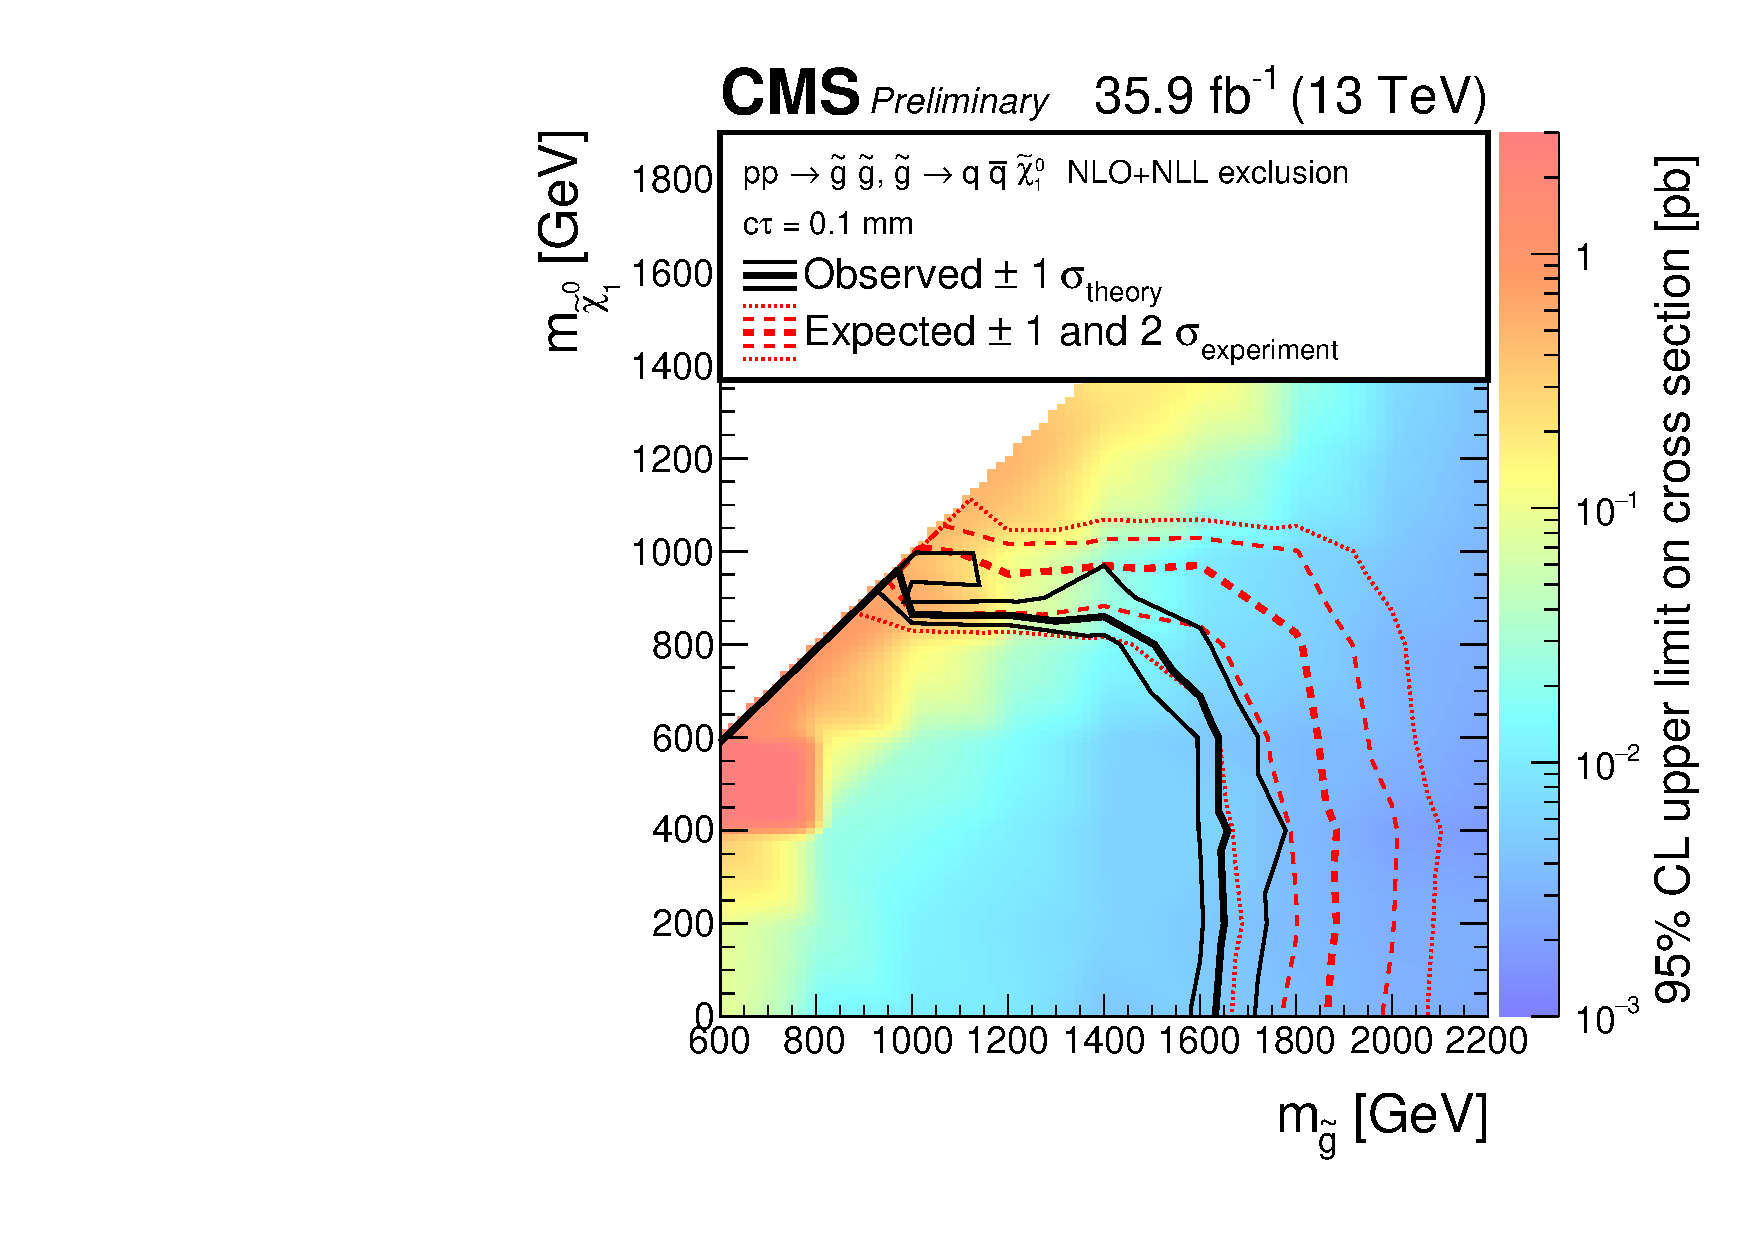
\includegraphics[width=0.33\textwidth]{Figures/T1qqqqLL_ctau-0p1_XSEC}\\
  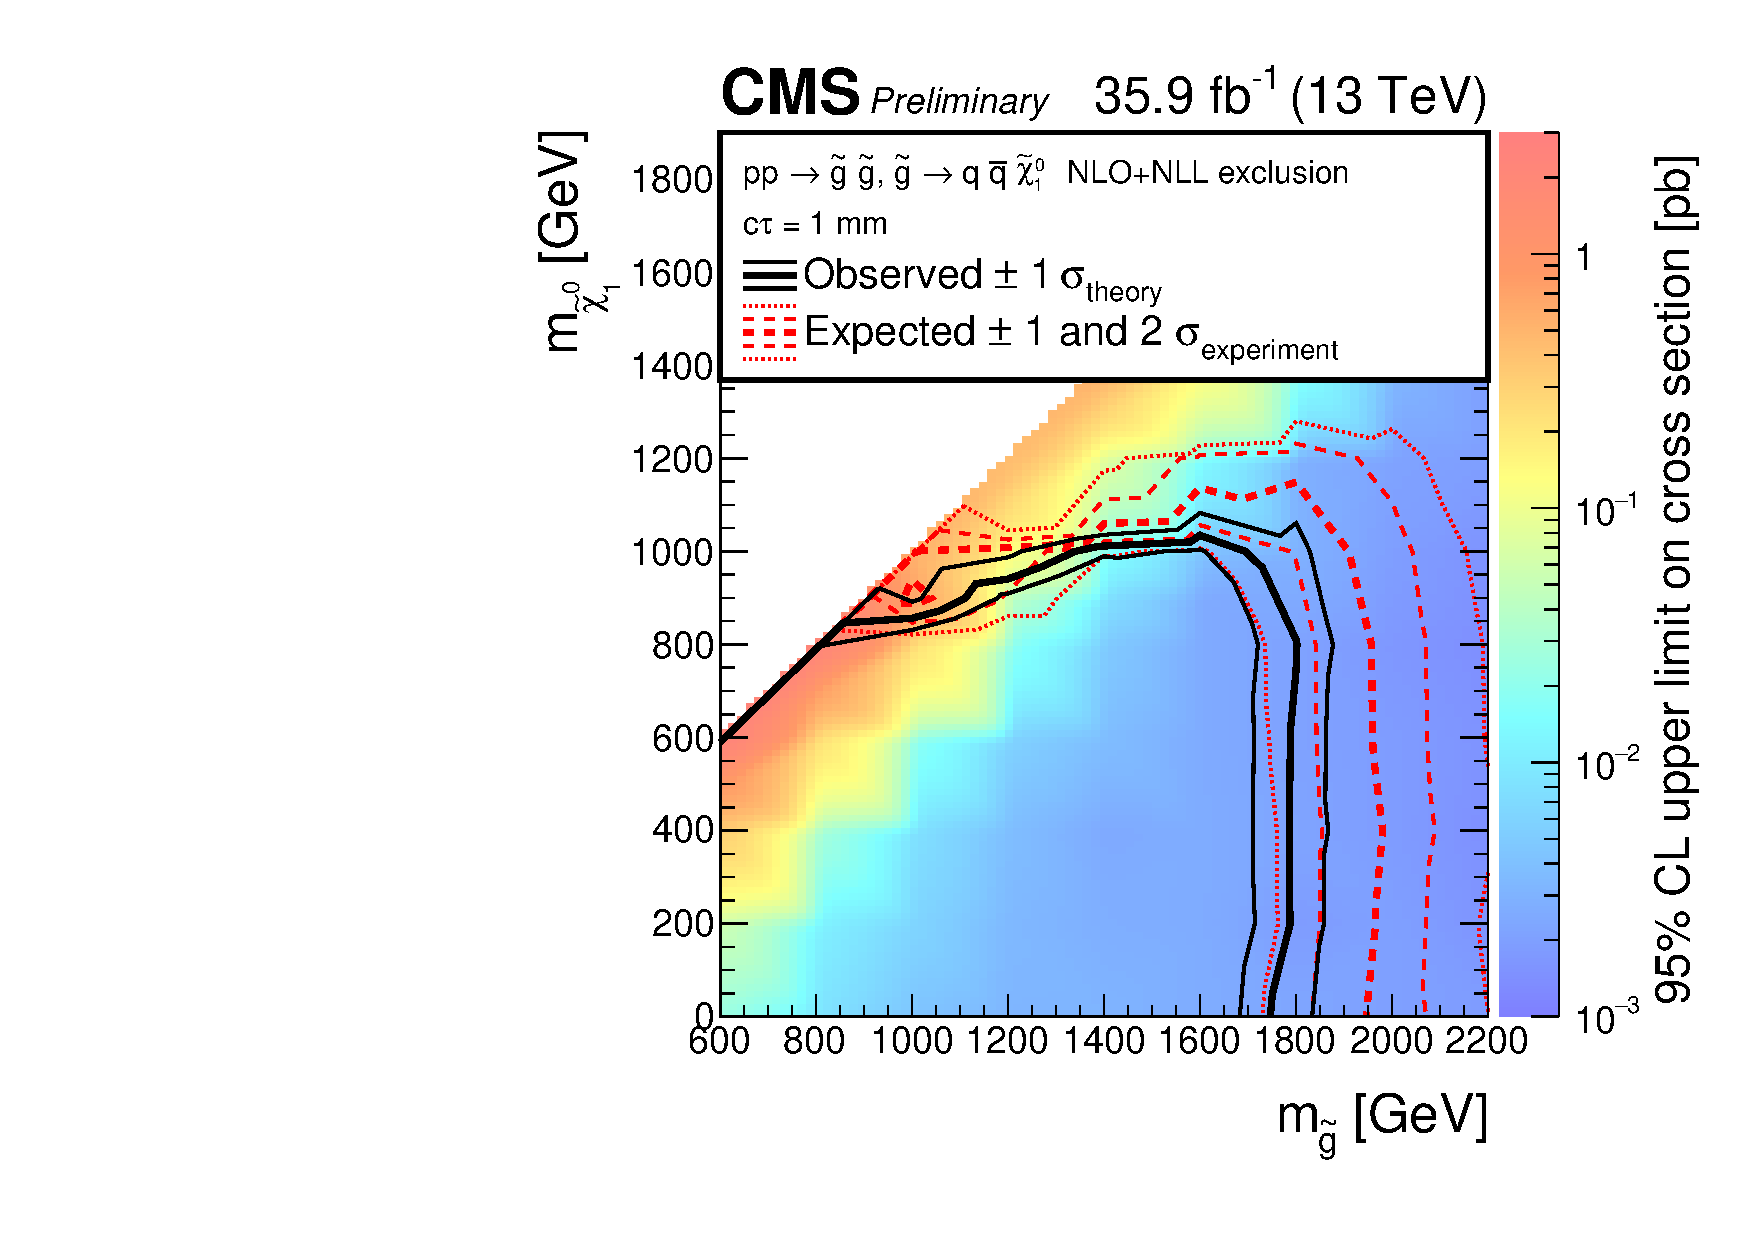
\includegraphics[width=0.33\textwidth]{Figures/T1qqqqLL_ctau-1_XSEC}~
  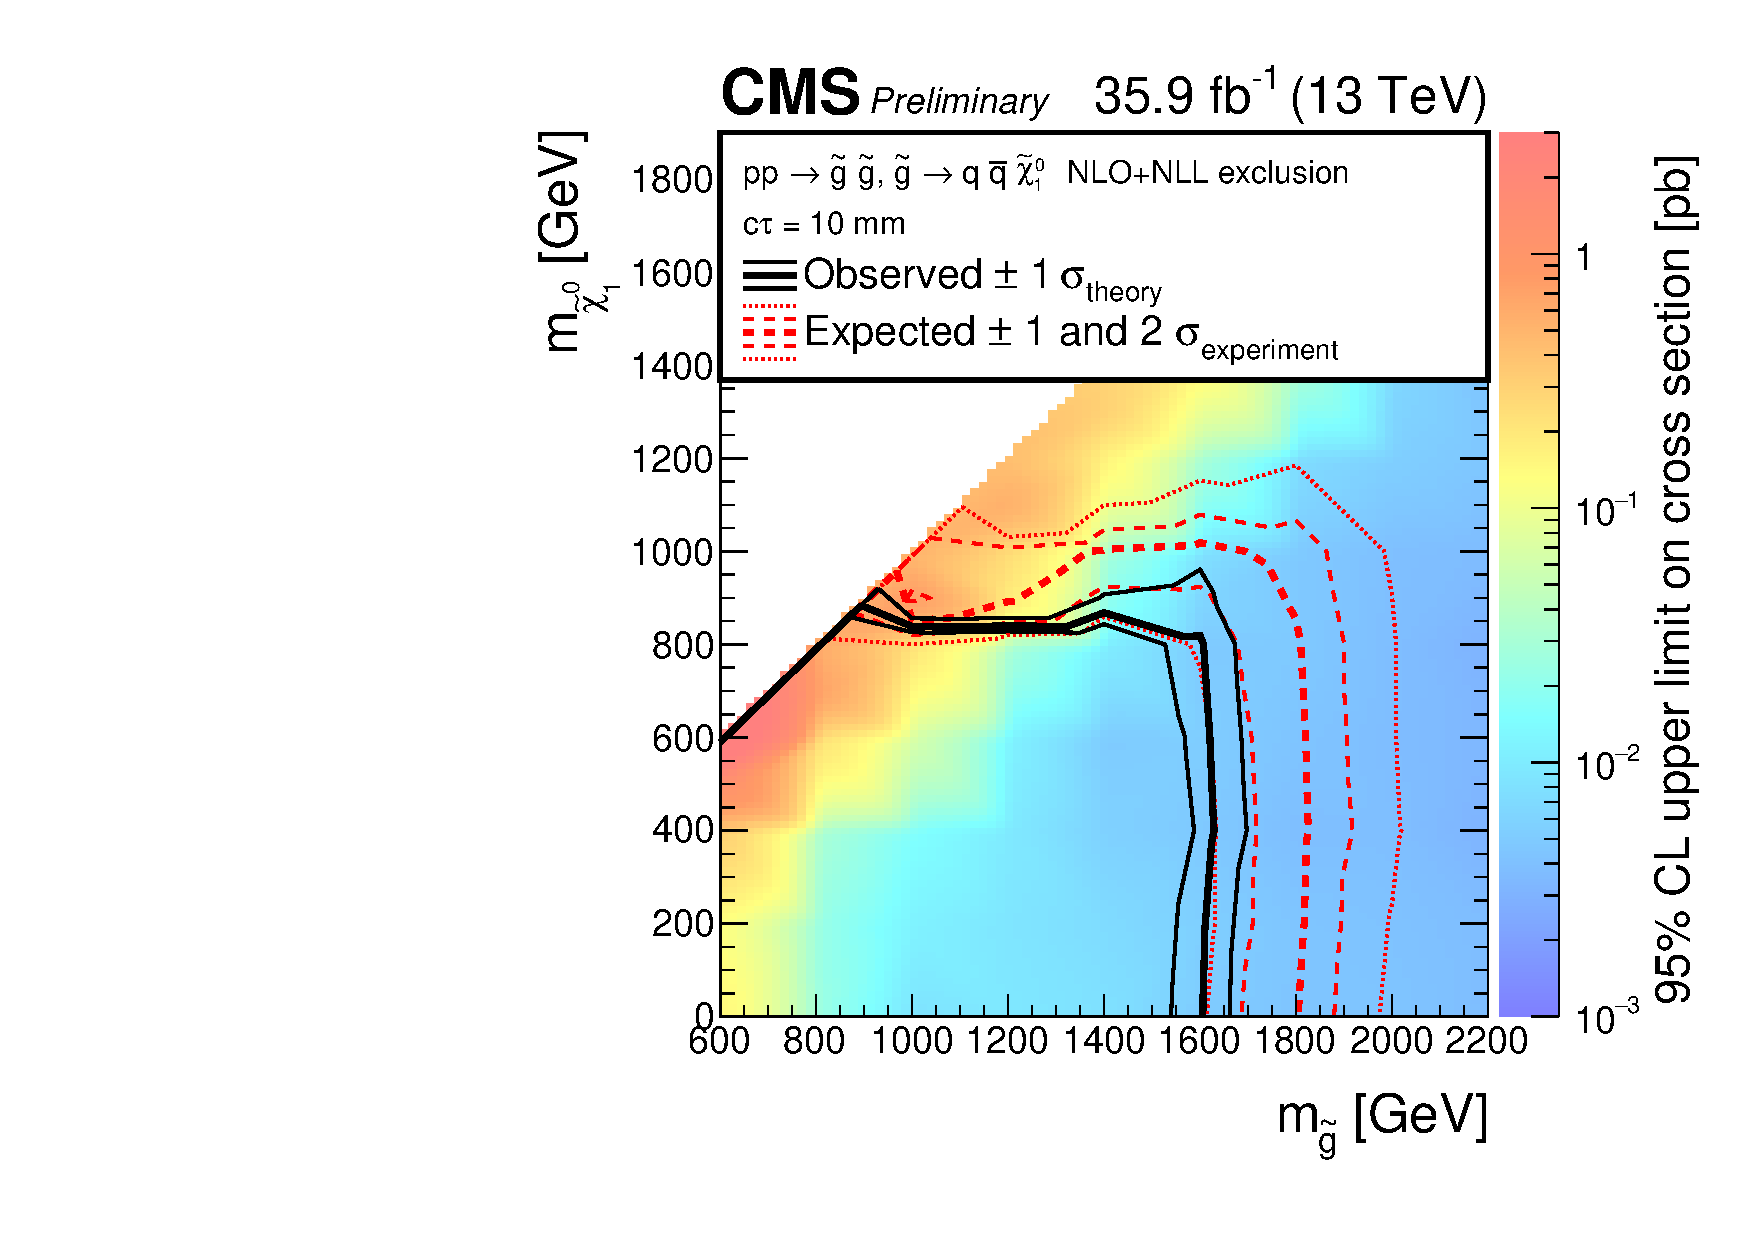
\includegraphics[width=0.33\textwidth]{Figures/T1qqqqLL_ctau-10_XSEC}~
  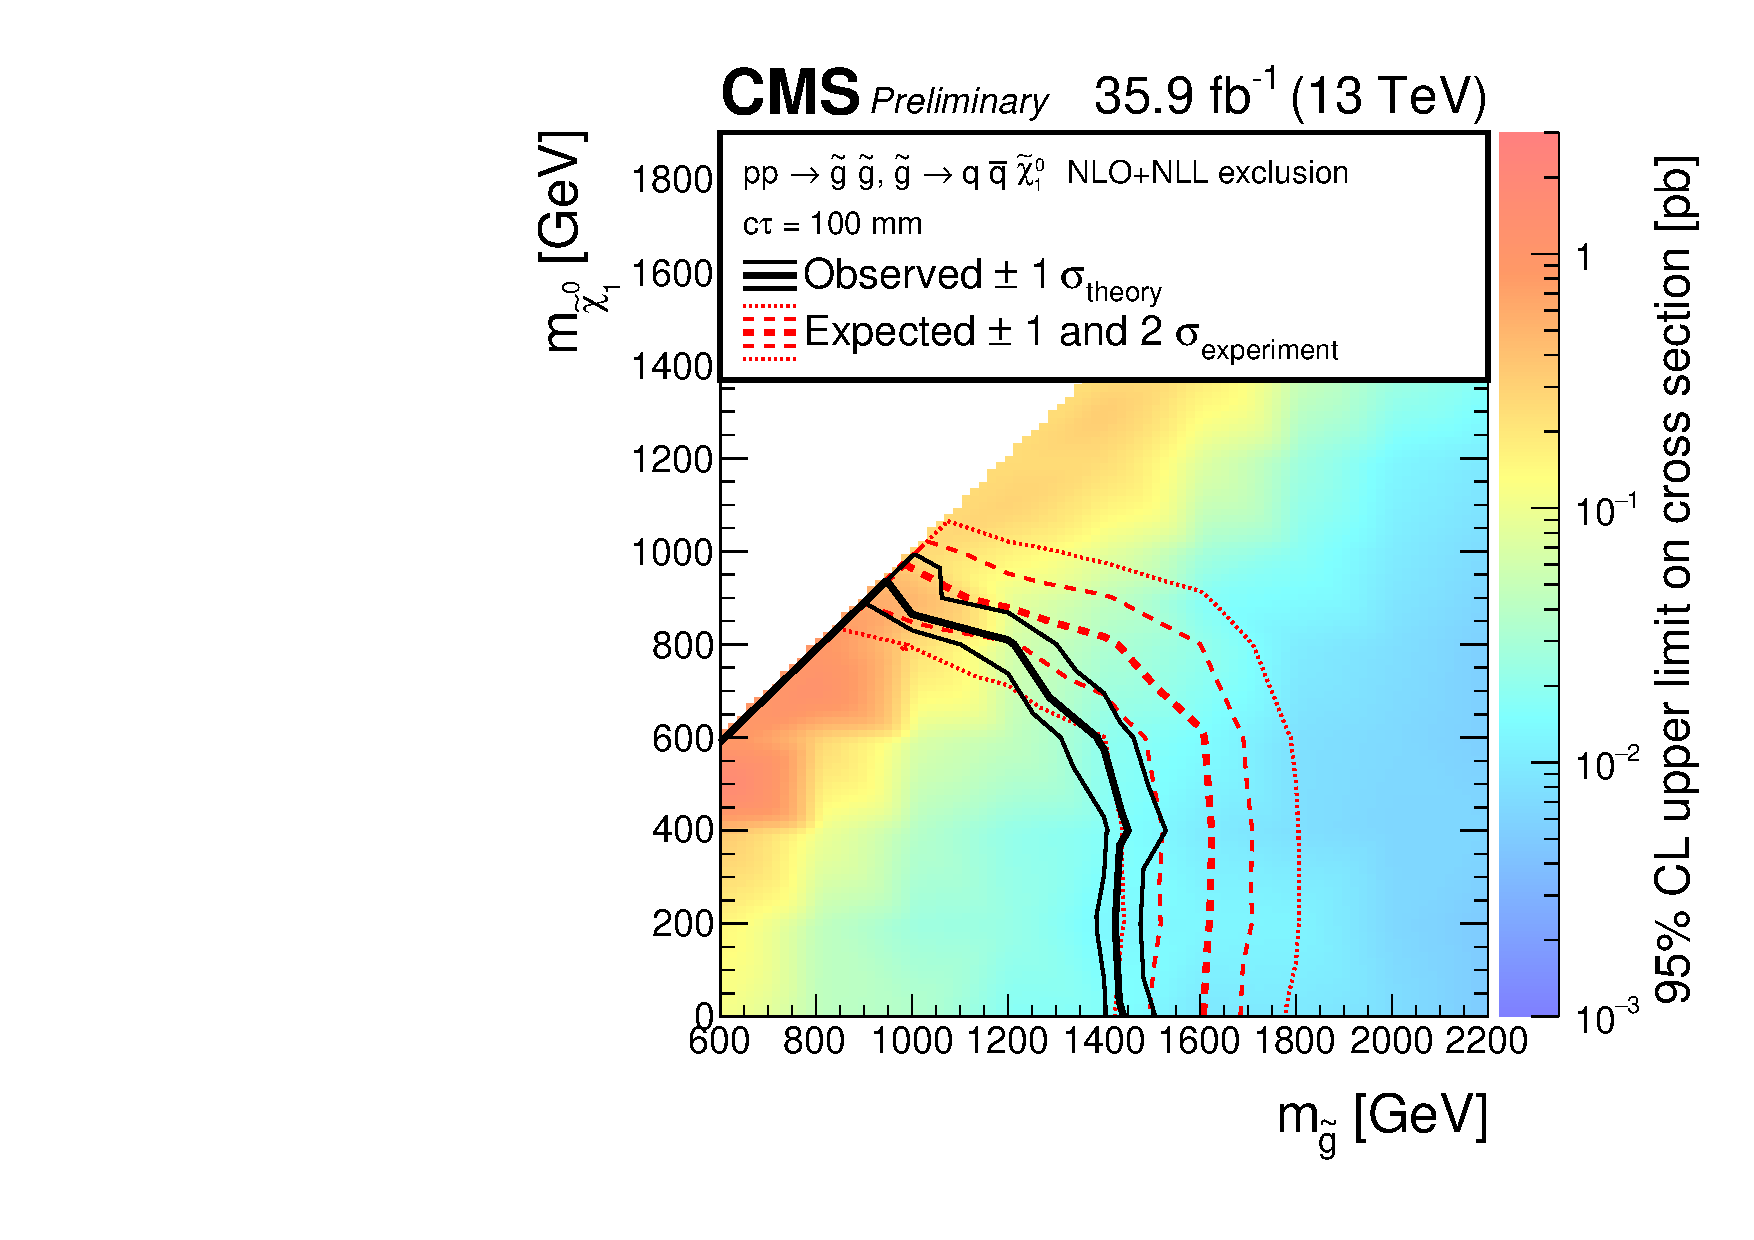
\includegraphics[width=0.33\textwidth]{Figures/T1qqqqLL_ctau-100_XSEC}\\
  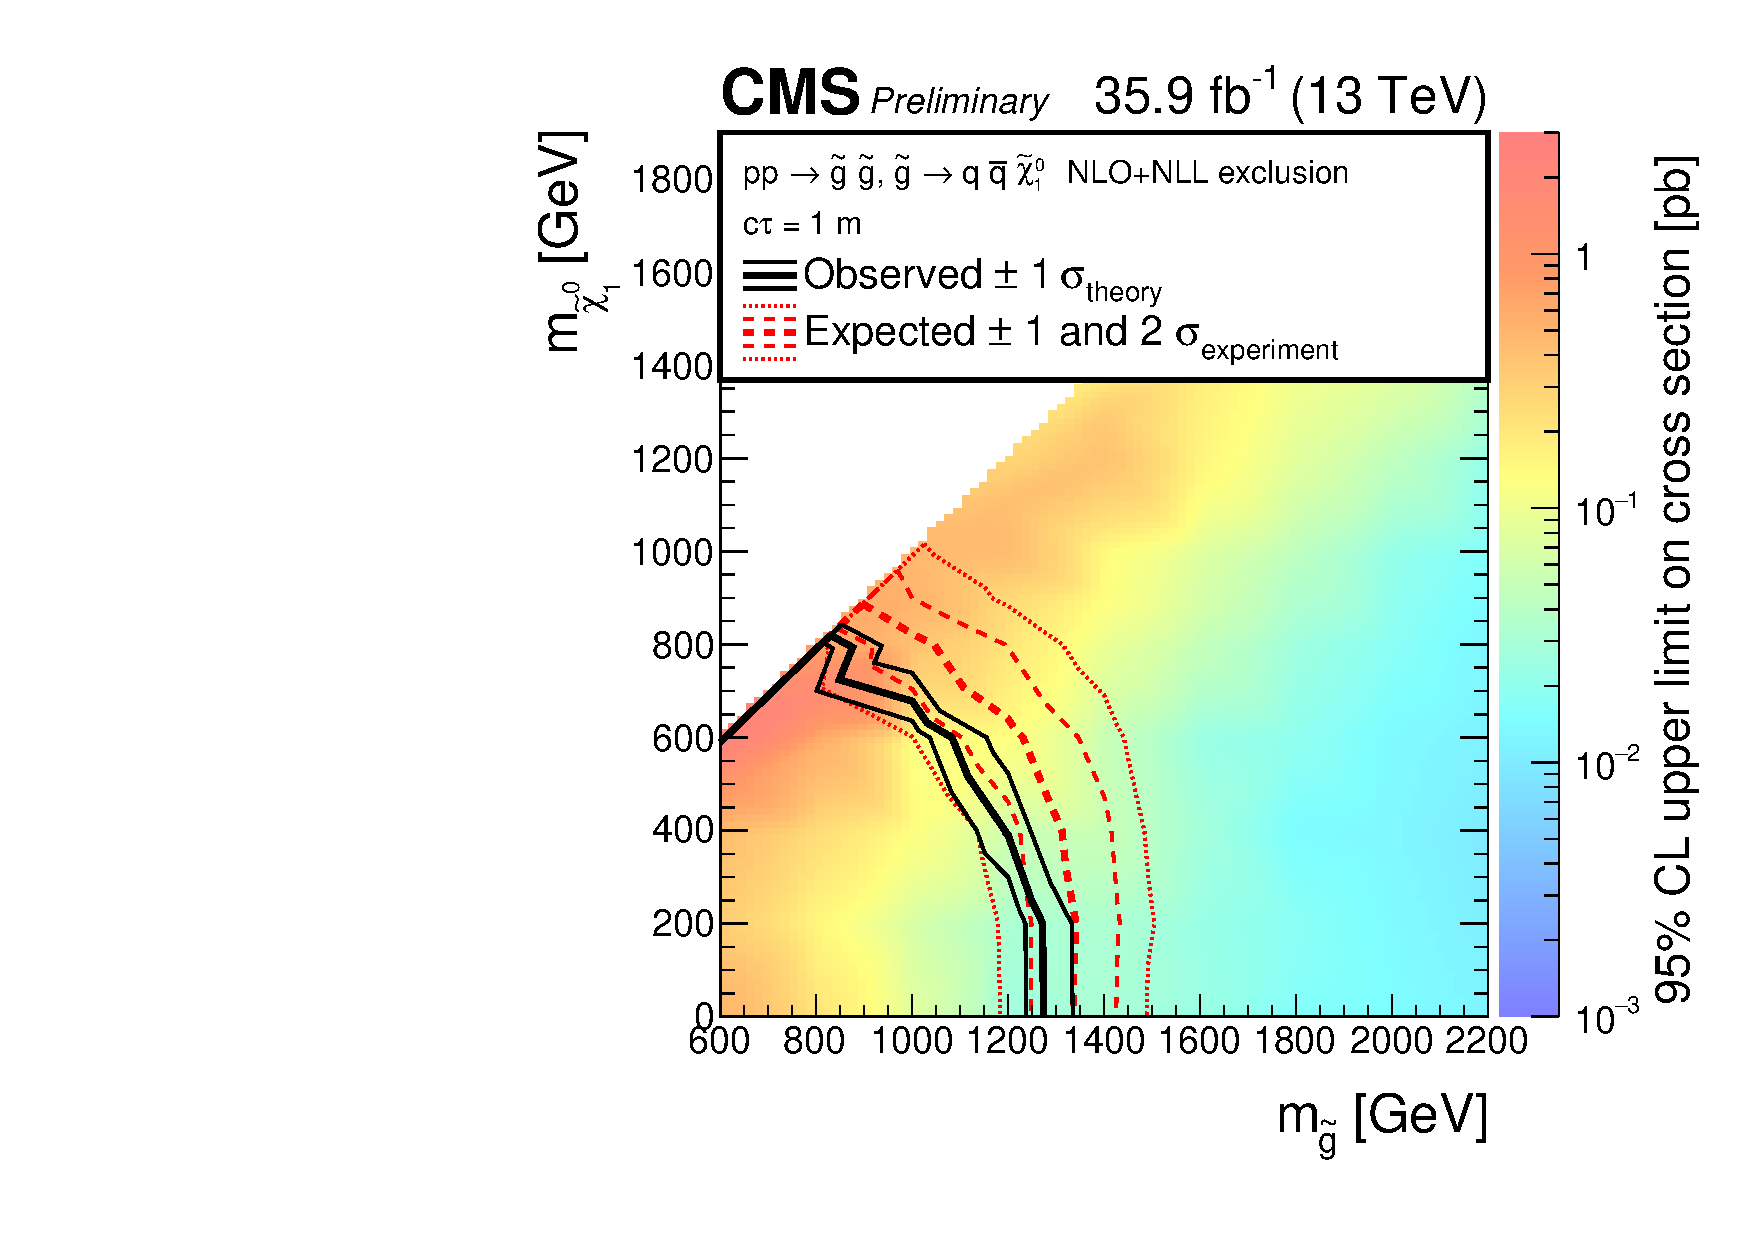
\includegraphics[width=0.33\textwidth]{Figures/T1qqqqLL_ctau-1000_XSEC}~
  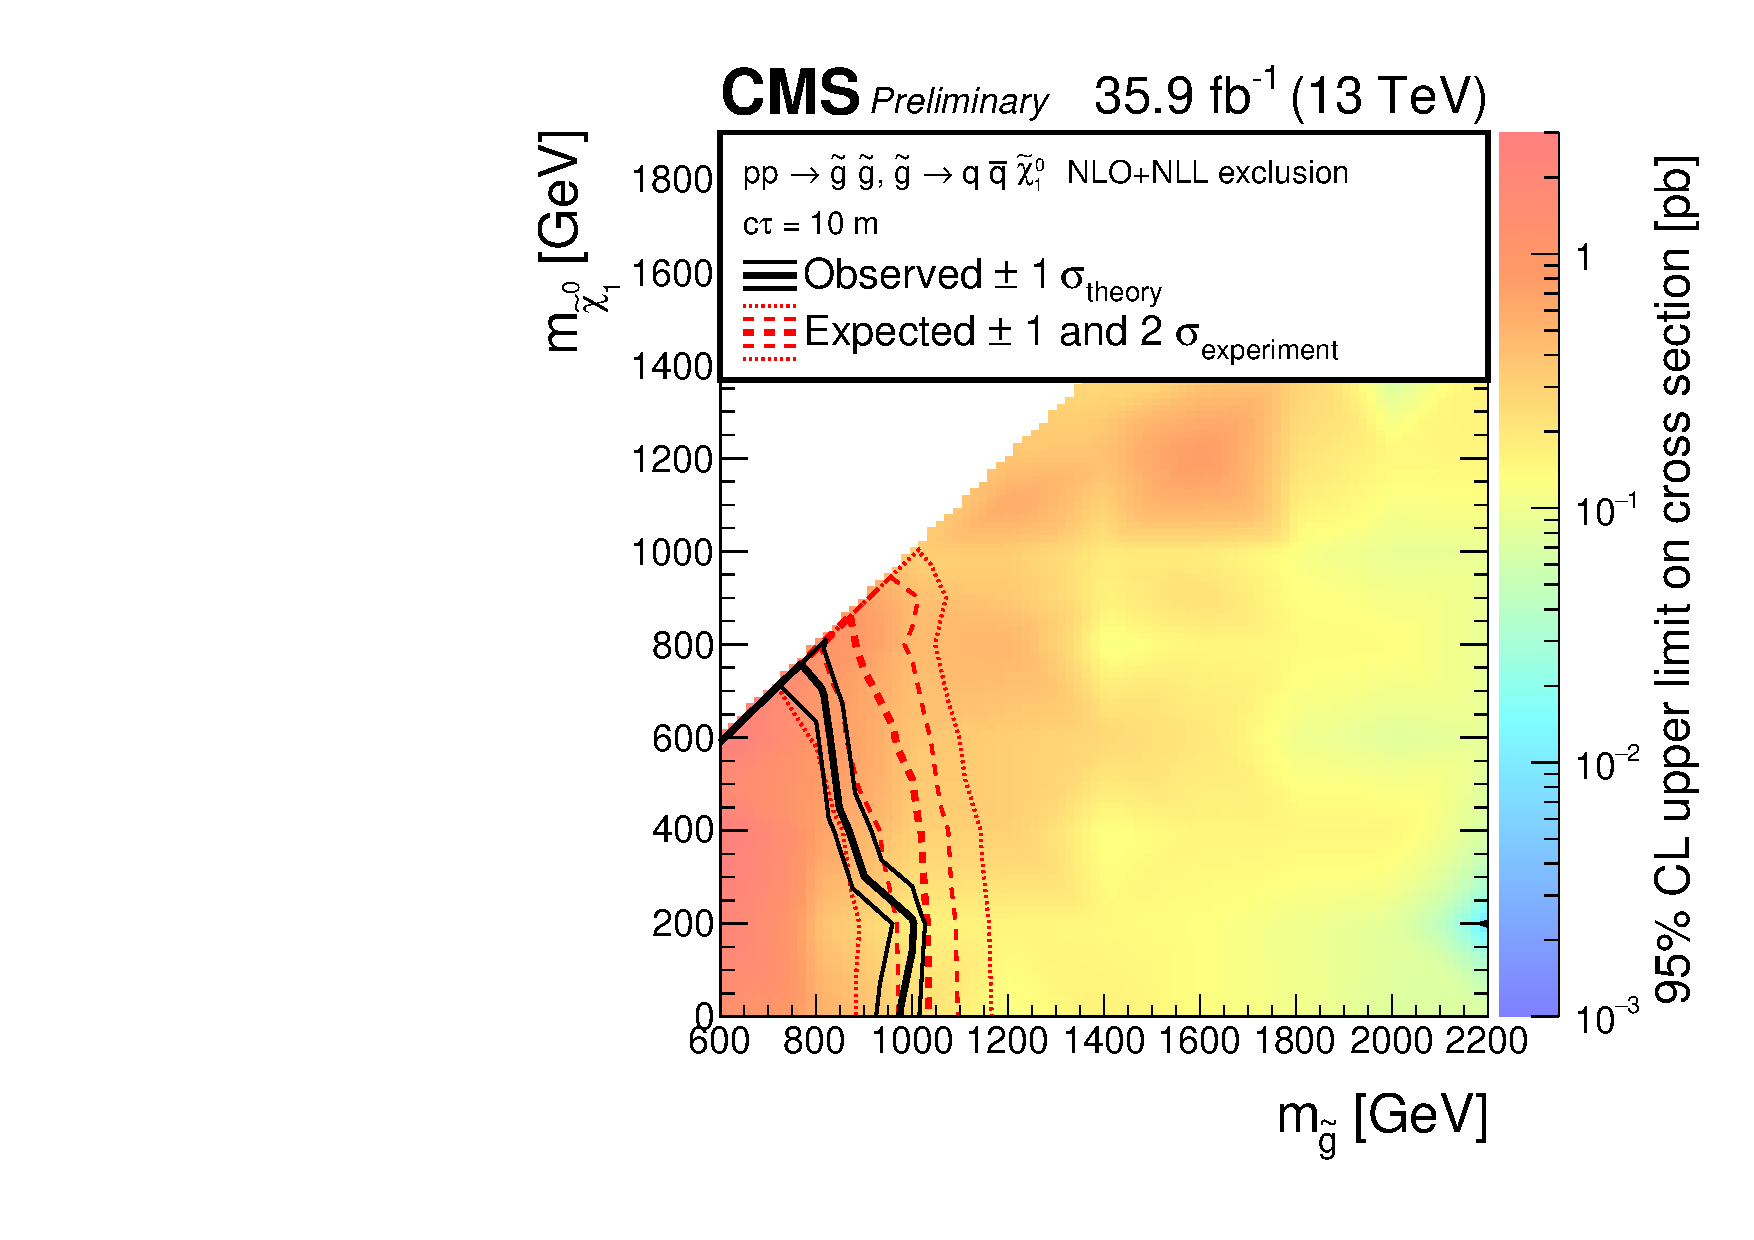
\includegraphics[width=0.33\textwidth]{Figures/T1qqqqLL_ctau-10000_XSEC}~
  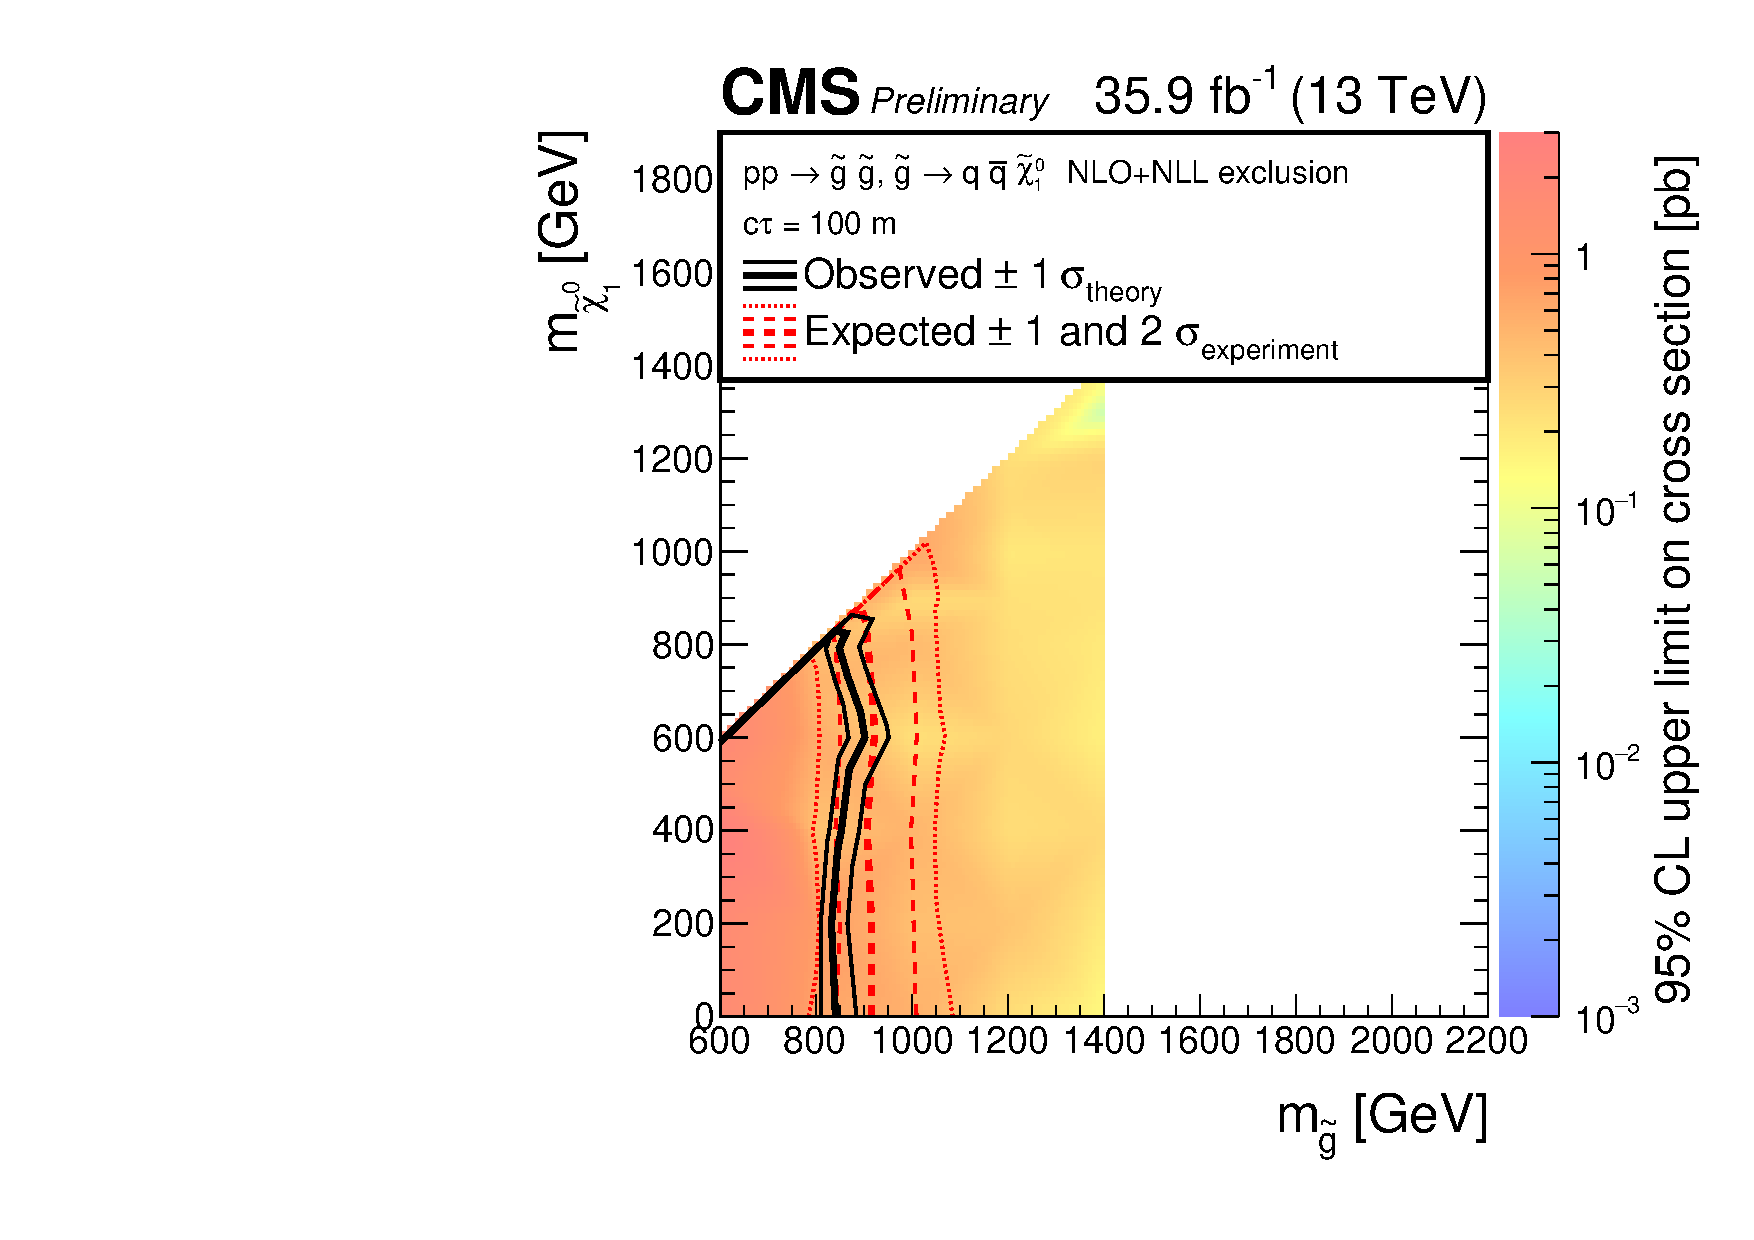
\includegraphics[width=0.33\textwidth]{Figures/T1qqqqLL_ctau-100000_XSEC}\\
  \caption{Observed upper limit in cross section at 95\% CL (indicated
    by the colour scale) as a function of the $\PSg$ and \chiz masses
    for simplified models that assume the production of pairs of
    long-lived $\PSg$ particles that each decay via highly virtual
    light-flavour squarks to the neutralino and SM particles
    (\texttt{T1qqqqLL}). The characteristic decay length $c\tau$ [mm]
    of the $\PSg$ varies for each subfigure: $10^{-6}\unit{m}$ (upper
    left), $10^{-5}\unit{m}$ (upper centre), $10^{-4}\unit{m}$ (upper
    right), $10^{-4}\unit{m}$ (middle left), $10^{-3}\unit{m}$ (middle
    centre), $10^{-2}\unit{m}$ (middle right), $10^{-1}\unit{m}$
    (lower left), $10^{0}\unit{m}$ (lower centre), and
    $10^{2}\unit{m}$ (lower right).  The black solid thick (thin) line
    indicates the observed mass exclusion regions assuming the nominal
    ($\pm$1 standard deviation in theory uncertainty) production cross
    section. The red dashed thick (thin) line indicates the median
    ($\pm$1 standard deviation in experimental uncertainty) expected
    mass exclusion regions.  }
  \label{fig:longlived} 
\end{figure} 

%_______________________________________________________________________________
%_______________________________________________________________________________
%_______________________________________________________________________________

\clearpage
\section{Summary}
\label{sec:summary}

An inclusive search for supersymmetry with the CMS experiment is
reported, based on a data sample of pp collisions collected in 2016 at
$\sqrt{s} = 13\TeV$ that corresponds to an integrated luminosity of
$35.9 \pm 0.9 \fbinv$. Final states with jets and significant
\ptvecmiss, as expected from the production and decay of massive
gluinos and squarks, have been analysed. Several kinematic variables
are used to suppress the multijet background to a subdominant level
with respect to all other standard model backgrounds. Candidate signal
events are categorized according to the number of reconstructed jets,
the number of jets identified to originate from bottom quarks, and the
scalar and vector sums of the transverse momentum of jets to provide
signal-to-background discrimination. The sum of standard model
backgrounds per bin has been estimated from a simultaneous binned
likelihood fit to event yields in the signal region and control
samples. The observed yields in the signal region are found to be in
agreement with the expected contributions from standard model
processes. Supplementary material is provided to aid the
interpretation of the result.

Limits are determined in the mass parameter space of simplified models
involving the gluino-mediated and direct production of light-flavour
and third-generation squark pairs. The masses of gluinos and
light-flavour, bottom and top squarks are probed up to 1900, X, 1075,
and 1040\GeV, respectively. Sensitivity to simplified models of split
supersymmetry is also demonstrated. These models assume the production
of long-lived gluinos that decay to yield final states containing
displaced vertices and missing transverse momenta from the undetected
neutralinos. This coverage is achieved with standard techniques for
event reconstruction. Gluinos with masses of at least ${\approx}1\TeV$
are excluded for lifetimes below ${\approx}10^{2}\unit{ns}$, providing
coverage that is complementary to other dedicated techniques at the
LHC. The strongest exclusions occur at lifetimes of
${\approx}10^{2}\unit{ns}$, with gluino masses probded up to X\TeV.

%_______________________________________________________________________________
%_______________________________________________________________________________
%_______________________________________________________________________________

\clearpage
\bibliography{auto_generated}

%_______________________________________________________________________________
%_______________________________________________________________________________
%_______________________________________________________________________________

\appendix

%_______________________________________________________________________________
%_______________________________________________________________________________
%_______________________________________________________________________________

\clearpage
\section*{Supplementary material} 

The following material is provided to aid the reinterpretation of the
result of this search. Table~\ref{tab:binning} specifies the nominal
binning schema used by this search. Table~\ref{tab:simplified}
summarises the search result based on a simplified binning schema.

\begingroup
\newcommand{\tmp}{\phantom{, 200}}
\begin{table}[!h]
  \topcaption{Summary of the nominal (\njet, \nb, \scalht, \mht)
    binning schema. Each entry (and the following entry, if present)
    signifies the lower (upper) bound of an \mht bin within a given
    (\njet, \nb, \scalht) bin. Unique or final entries represent \mht
    bins unbounded from above. A dash (--) signifies that the \scalht 
    bin in a given (\njet, \nb) category is not used in the analysis,
    in which case counts in high-\scalht bins are integrated into the
    adjacent lower-\scalht bin. For monojet events, $\scalht \equiv
    \mht$. 
  }
  \label{tab:binning}
  \small
  \centering
  \begin{tabular}{rrlllll}
    \hline
    \njet      & \nb       & \multicolumn{5}{c}{\scalht [GeV]}                                        \\ 
    \cline{3-7}
    &           & 200 & 400      & 600           & 900                & 1200               \\
    \hline
    1          & 0         & 200 & 400 \tmp & 600 \tmp \tmp & 900 \tmp \tmp \tmp & --                 \\ 
    1          & 1         & 200 & 400 \tmp & 600 \tmp \tmp & --                 & --                 \\ 
    ${\geq}2a$ & 0         & 200 & 200, 400 & 200, 400, 600 & 200, 900 \tmp \tmp & --                 \\ 
    ${\geq}2a$ & 1         & 200 & 200, 400 & 200, 400, 600 & 200, 900 \tmp \tmp & --                 \\ 
    ${\geq}2a$ & 2         & 200 & 200, 400 & 200, 400, 600 & 200, 900 \tmp \tmp & --                 \\ 
    ${\geq}2a$ & ${\geq}3$ & 200 & 200, 400 & 200, 400, 600 & --                 & --                 \\ 
    2          & 0         & 200 & 200, 400 & 200, 400, 600 & 200, 400, 600, 900 & 200, 400, 600, 900 \\ 
    2          & 1         & 200 & 200, 400 & 200, 400, 600 & 200, 400, 600, 900 & 200, 400, 600, 900 \\ 
    2          & 2         & 200 & 200, 400 & 200, 400, 600 & --                 & --                 \\ 
    3          & 0         & 200 & 200, 400 & 200, 400, 600 & 200, 400, 600, 900 & 200, 400, 600, 900 \\ 
    3          & 1         & 200 & 200, 400 & 200, 400, 600 & 200, 400, 600, 900 & 200, 400, 600, 900 \\ 
    3          & 2         & 200 & 200, 400 & 200, 400, 600 & 200, 400, 600, 900 & 200, 400, 600, 900 \\ 
    3          & 3         & 200 & 200, 400 & 200, 400, 600 & --                 & --                 \\ 
    4          & 0         & --  & 200, 400 & 200, 400, 600 & 200, 400, 600, 900 & 200, 400, 600, 900 \\ 
    4          & 1         & --  & 200, 400 & 200, 400, 600 & 200, 400, 600, 900 & 200, 400, 600, 900 \\ 
    4          & 2         & --  & 200, 400 & 200, 400, 600 & 200, 400, 600, 900 & 200, 400, 600, 900 \\ 
    4          & ${\geq}3$ & --  & 200, 400 & 200, 400, 600 & 200, 400, 600, 900 & --                 \\ 
    5          & 0         & --  & 200, 400 & 200, 400, 600 & 200, 400, 600 \tmp & 200, 400, 600, 900 \\ 
    5          & 1         & --  & 200, 400 & 200, 400, 600 & 200, 400, 600 \tmp & 200, 400, 600, 900 \\ 
    5          & 2         & --  & 200, 400 & 200, 400, 600 & 200, 400, 600 \tmp & 200, 400, 600, 900 \\ 
    5          & 3         & --  & 200, 400 & 200, 400, 600 & 200, 400, 600 \tmp & --                 \\ 
    5          & ${\geq}4$ & --  & 200, 400 & --            & --                 & --                 \\ 
    ${\geq}6$  & 0         & --  & 200 \tmp & 200, 400 \tmp & 200, 400, 600 \tmp & 200, 400, 600, 900 \\ 
    ${\geq}6$  & 1         & --  & 200 \tmp & 200, 400 \tmp & 200, 400, 600 \tmp & 200, 400, 600, 900 \\ 
    ${\geq}6$  & 2         & --  & 200 \tmp & 200, 400 \tmp & 200, 400, 600 \tmp & 200, 400, 600, 900 \\ 
    ${\geq}6$  & 3         & --  & 200 \tmp & 200, 400 \tmp & 200, 400, 600 \tmp & 200, 400, 600, 900 \\ 
    ${\geq}6$  & ${\geq}4$ & --  & 200 \tmp & --            & --                 & --                 \\ 
    \hline
  \end{tabular}
\end{table}
\endgroup

\begingroup
\renewcommand*{\arraystretch}{1.1}
\begin{table}[!t]
  \topcaption{Observed counts of candidate signal events and SM
    expectations determined from the CR-only fit using the simplified
    binning schema, as a function of \njet, \nb, and \mht. All counts
    are integrated over \scalht. The uncertainties include both
    statistical and systematic contributions.  
  }
  \label{tab:simplified}
  \centering
  \begin{tabular}{rrlr@{}lr@{}lr@{}lr@{}l}
    \hline
    \njet          & \nb       &      & \multicolumn{8}{c}{\mht [GeV]}                                                                     \\
    \cline{4-11}
                   &           &      & 200      &                 & 400    &               & 600   &               & 900   &              \\
    \hline
    =1, ${\geq}2a$ & 0         & Data & 411184   &                 & 11448  &               & 1116  &               & 111                  \\
                   &           & SM   & $360000$ & $\,\pm\, 35000$ & $9990$ & $\,\pm\, 890$ & $910$ & $\,\pm\, 300$ & $107$ & $\,\pm\, 64$ \\[0.2ex]
    =1, ${\geq}2a$ & ${\geq}1$ & Data & 31174    &                 & 769    &               & 96    &               & 16                   \\
                   &           & SM   & $25500$  & $\,\pm\, 2300$  & $649$  & $\,\pm\, 61$  & $65$  & $\,\pm\, 20$  & $11$  & $.4 \pm 6.7$ \\[0.2ex]
    =2, =3         & =0, =1    & Data & 66955    &                 & 5946   &               & 903   &               & 100                  \\
                   &           & SM   & $58000$  & $\,\pm\, 10000$ & $5410$ & $\,\pm\, 970$ & $860$ & $\,\pm\, 330$ & $113$ & $\,\pm\, 76$ \\[0.2ex]
    =2, =3         & ${\geq}2$ & Data & 1045     &                 & 70     &               & 6     &               & 0                    \\
                   &           & SM   & $870$    & $\,\pm\, 130$   & $56$   & $.9 \pm 8.8$  & $7$   & $.1 \pm 2.6$  & $1$   & $.0 \pm 0.7$ \\[0.2ex]
    =4, =5         & =0, =1    & Data & 9546     &                 & 1734   &               & 315   &               & 44                   \\
                   &           & SM   & $10490$  & $\,\pm\, 1100$  & $1880$ & $\,\pm\, 250$ & $320$ & $\,\pm\, 110$ & $40$  & $\,\pm\, 27$ \\[0.2ex]
    =4, =5         & ${\geq}2$ & Data & 1012     &                 & 93     &               & 4     &               & 3                    \\
                   &           & SM   & $970$    & $\,\pm\, 120$   & $81$   & $.2 \pm 9.4$  & $8$   & $.4 \pm 2.4$  & $1$   & $.2 \pm 0.7$ \\[0.2ex]
    ${\geq}6$      & =0, =1    & Data & 758      &                 & 141    &               & 33    &               & 5                    \\
                   &           & SM   & $910$    & $\,\pm\, 180$   & $167$  & $\,\pm\, 71$  & $33$  & $\,\pm\, 25$  & $4$   & $.2 \pm 5.4$ \\[0.2ex]
    ${\geq}6$      & ${\geq}2$ & Data & 197      &                 & 14     &               & 3     &               & 0                    \\
                   &           & SM   & $189$    & $\,\pm\, 39$    & $16$   & $.9 \pm 4.8$  & $2$   & $.1 \pm 1.2$  & $0$   & $.2 \pm 0.3$ \\
    \hline
  \end{tabular}
\end{table}
\endgroup

\begin{figure}[!b]
  \centering
  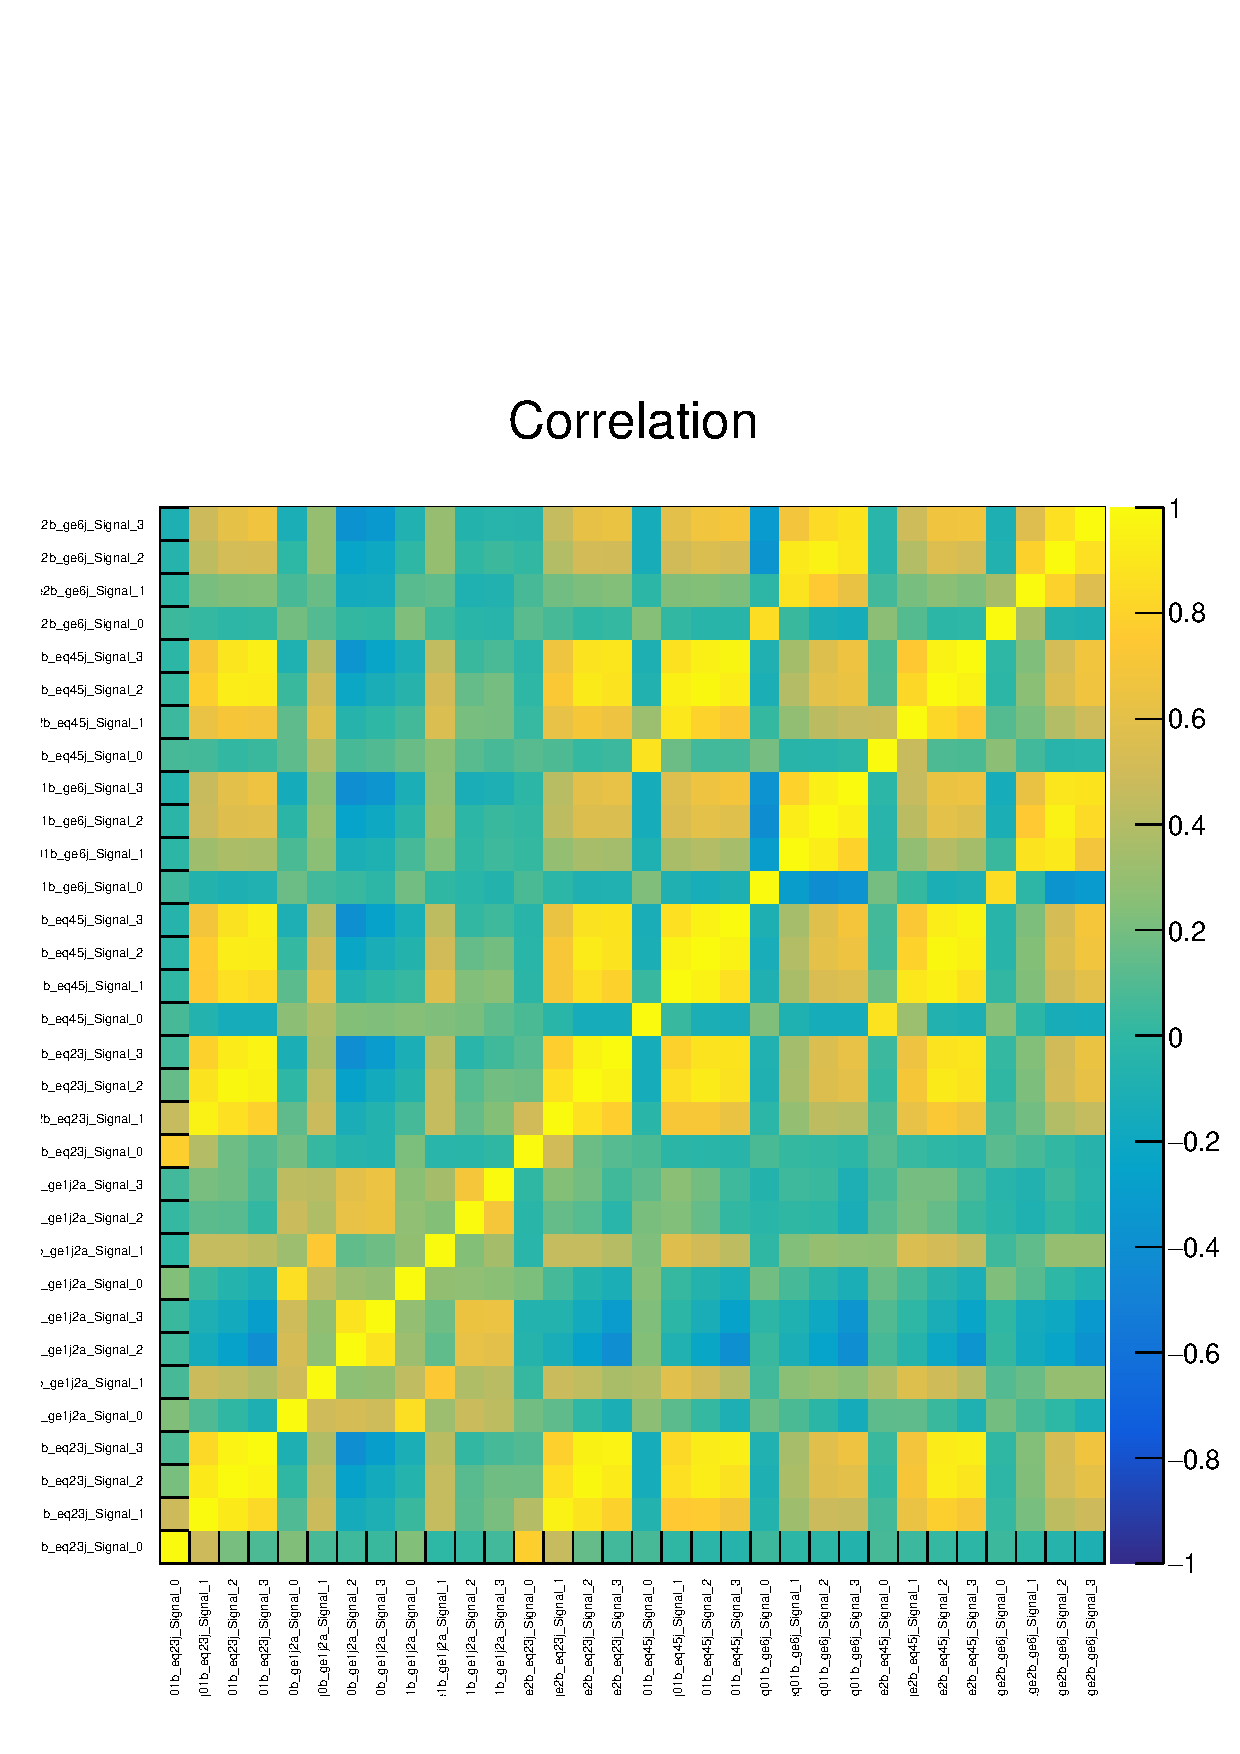
\includegraphics[width=0.5\textwidth]{Figures/correlation.pdf}
  \caption{Correlation matrix for the SM background estimates obtained
    using the simplified binning schema, determined from the CR-only
    fit.  }
  \label{fig:correlation}
\end{figure} 
